%% Road to VPhO 2023 Template

\documentclass[12pt]{article}
\usepackage[utf8]{vietnam}
%\usepackage[english]{babel}
\usepackage[T5]{fontenc}
\usepackage[top=2cm, bottom=2cm, left=2cm,right=2cm]{geometry} %%%% Margin %%%%%
\usepackage[dvipsnames]{xcolor}
\usepackage[pdftex]{graphicx}
\usepackage{wrapfig}
\usepackage{tcolorbox}
\usepackage{amssymb}
\usepackage{eqnarray}

\usepackage{subcaption}
\usepackage{array, lipsum, bibentry,fancyhdr}
\setlength{\parindent}{0pt}
\usepackage{enumitem}
\usepackage[noframe]{showframe}
\usepackage{framed}
\usepackage{titling}
\usepackage{float}
\usepackage{multicol}
\usepackage{authblk}
\usepackage{sectsty}
\usepackage{eqparbox}
\usepackage{ulem} 

%%%%%%%%%% Math %%%%%%%%%%%%%
\usepackage{mathtools}
\usepackage{amsmath}
\usepackage{siunitx} % unit


%%%%%%%%%% Pictures drawing %%%%%%%%%%%%%

\usepackage{pgfplots} %%%%%% Regression %%%%
\pgfplotsset{compat = newest}
\usepackage{pgfplotstable}
\usepackage{tikz}
\usepackage{tikz-3dplot} %%%%%% Draw %%%%%%
\usepackage{tikz,tkz-euclide}
\usetikzlibrary{arrows,calc,patterns}
\usetikzlibrary{quotes,angles}
\usetikzlibrary{shapes.geometric}
\usepackage{circuitikz} %%%%% Circuit %%%%
\usetikzlibrary{decorations.pathmorphing,patterns}

\setlength{\unitlength}{1cm}

%%%%%%%%%% Ref & Hyperlink %%%%%%%%%%%%%
\usepackage{url}
\usepackage{hyperref}
\usepackage{natbib}
\hypersetup{
	colorlinks=true,
	linkcolor=blue,
	filecolor=blue,      
	urlcolor=blue,
    citecolor=blue,
	pdftitle={Overleaf Example},
	pdfpagemode=FullScreen,
}

%%%%%%%%%% Set Counter and Reference Equation %%%%%%%%%%

\usepackage{xassoccnt}
\newcounter{totalequations}
\DeclareAssociatedCounters{equation}{totalequations}
\let\theOldHequation\theHequation
\renewcommand{\theHequation}{\theOldHequation::\number\value{totalequations}}

%%%%%%%%%% Header & Footer %%%%%%%%%%%%%

\setlength{\headheight}{10mm}
\RequirePackage{fancyhdr}  % Needed to define custom headers/footers
\RequirePackage{lastpage}  % Number of pages in the document
\pagestyle{fancy}          % Enables the custom headers/footers
% Headers
\lhead{
\includegraphics[width=.8in]{xPhO.png}}%
\chead{}%
\rhead{\small\sffamily\bfseries{Hướng tới VPhO 43} --- \thepage/\pageref{LastPage}}
% Footers
\lfoot{}%
\cfoot{}%
\rfoot{}%
\renewcommand{\headrulewidth}{1pt}% % header rule
\renewcommand{\footrulewidth}{1pt}% % footer rule

% \pagestyle{fancy}
% 	\fancyhead[L]{\empty}
% 	\fancyhead[R]{\empty}
% 	\fancyhead[C]{\empty}
% 	\fancyfoot[C]{\empty}
% 	\fancyfoot[L]{\empty}
% 	\renewcommand{\headrulewidth}{0pt}
% 	\fancyfoot[C]{\normalcolor{\thepage/\pageref{LastPage}}}
% 	\setcounter{page}{1}

%%%%%%%%%% Color setup %%%%%%%%%%%%%
\usepackage[dvipsnames]{xcolor}
\usepackage{tcolorbox}

\RequirePackage{xcolor}
\definecolor{wsdred}{HTML}{8E1728}
\definecolor{wsdgrey}{HTML}{75787B}
\definecolor{battleshipgrey}{rgb}{0.52, 0.52, 0.51}
\renewcommand{\normalcolor}{\color{wsdred}}
\colorlet{ColorOr}{white}

\begin{document}

%% Title %%
{\fontsize{50}{24}\fontfamily{phv}\fontseries{b}
\LARGE \normalcolor{ \textbf{Hướng tới VPhO 43} } }

\textcolor{blue}{\textbf{\textit{Câu lạc bộ vật lý xPhO}}}
%%%%

{\normalcolor\textbf{CÂU 1 (4 điểm)}}\vspace{1.5mm}

\setcounter{equation}{0}
Một quả lựu đạn đang đứng yên ở độ cao $H$ so với mặt đất thì phát nổ và bắn ra các mảnh đạn giống nhau với cùng tốc độ $v_0$, phân bố các mảnh đạn khi văng ra là đẳng hướng. Gia tốc trọng trường là $\Vec{g}$.
\begin{enumerate}[label=\textbf{\alph*,}]\itemsep0em
    \item Xác định phương trình mặt cong ba chiều biểu diễn ranh giới giữa \textit{vùng an toàn} và \textit{vùng nguy hiểm}, tức là trong vùng an toàn thì mảnh đạn sẽ không thể bay tới, ngược lại với vùng nguy hiểm. Vẽ phác dạng đồ thị của đường ranh giới, ghi chú thích và các điểm đặc biệt.
    \item Sau khi các mảnh đạn rơi hết xuống đất, xác định bán kính $R$ của vùng đạn đã rơi trên mặt đất.
    \item Giả sử rằng lựu đạn chứa $M$ khối lượng đạn nổ trong một góc nón nhỏ hướng lên trên với góc mở $2\alpha_0 \ll 1$, bom nổ trên mặt đất ($H = 0$). Chứng minh rằng phân bố khối lượng mặt $\rho(r)$ (khai triển tới thành phần bậc hai $r^2$) của đạn trên mặt đất khi tất cả mảnh đạn đã rơi xuống đất có dạng như sau
    $$\rho(r) \approx \rho_0 (1 + \beta r^2),$$

    hãy biểu diễn $\rho_0$ và $\beta$ theo các thông số đã biết.
\end{enumerate}

\textit{Có thể sử dụng xấp xỉ sau:} $\displaystyle \sin \alpha \approx \alpha \left(1 - \frac{1}{6} \alpha^2 \right)$.

\begin{flushright}
    (Biên soạn bởi Zinc)
\end{flushright}
\setcounter{equation}{0}
\begin{center}
    \normalcolor{\textbf{Bài giải}}
\end{center}
\textbf{a,} Ta đặt $r = \sqrt{x^2 + y^2}$ là toạ độ khoảng cách trong mặt phẳng $Oxy$. Từ phương trình ném xiên, tuân theo định luật Newton II, ta có phương trình chuyển động của mảnh đạn:
\begin{align}
    z &= -\frac{1}{2} g t^2 + v_0 \sin \theta t + H, \label{1}\\
    r&= v_0 \cos \theta t. \label{2}
\end{align}

Thay (\ref{1}) vào (\ref{2}) ta thu được phương trình quỹ đạo của mảnh đạn là
\begin{align}
    z = H- \frac{g}{2 v_0^2 \cos^2 \theta} r^2 + r \tan \theta. \label{3}
\end{align}

Ta có thể viết (\ref{3}) thành phương trình tam thức bậc hai với biến $\tan \theta$ như sau
\begin{align}
    - \frac{g r^2}{2 v_0^2} \tan^2 \theta + r \tan \theta - \left( \frac{g r^2}{2 v_0} + z -H \right) = 0.\label{4}
\end{align}

\begin{itemize}\itemsep0em
\item Bên ngoài ranh giới, tức vùng an toàn, thì phương trình (\ref{4}) vô nghiệm.

\item Bên trong ranh giới, tức vùng nguy hiểm, thì phương trình (\ref{4}) có hai nghiệm phân biệt.

\item Tại ranh giới thì phương trình (\ref{4}) là nghiệm kép, tức là $\Delta = 0$.
\end{itemize}



Từ nhận xét trên ta có phương trình
\begin{align}
    \Delta &= r^2 - 4 \frac{gr^2}{2 v_0^2} \left( \frac{gr^2}{2v_0^2} + z-H \right) = 0,\\
    \Rightarrow z &= H + \frac{v_0^2}{2g} - \frac{gr^2}{2 v_0^2} = H + \frac{v_0^2}{2g} - \frac{g}{2 v_0^2} (x^2 + y^2).\label{10}
\end{align}

Hình bên dưới là mô phỏng đường ranh giới an toàn của bom nổ.

\begin{center}
    \begin{tikzpicture}
\begin{axis}[
xlabel=$x$, ylabel=$y$, zlabel=$z$, 
xmin=-19, xmax=19,
ymin=-19, ymax=19,
zmin=-1, zmax=110,
x={(-0.125cm,-0.05cm)}, y={(0.125cm,-0.05cm)}, z={(0cm,0.05cm)},
axis lines=middle,
every axis x label/.style={  at={(ticklabel* cs:1.05)},  },
every axis y label/.style={  at={(ticklabel* cs:1.05)},  },
every axis z label/.style={  at={(ticklabel* cs:1.05)},  },
]
% Paraboloid
\addplot3[surf,
shader=flat, draw=lightgray, fill=green!80, ultra thin, 
left color=green, right color=green, middle color=green!25, 
opacity=0.5, fill opacity=0.5,
data cs=polar, domain=0:360, 
y domain=0:10,
restrict z to domain=0:101, 
](x, y, 100-y^2);

% Plane 
\addplot3[surf, shader=faceted,
color=orange, 
opacity=0.01, fill opacity=0.4, 
domain=-10:10, 
](x,y,75);

% Circle at plane
\addplot3[red, smooth, 
domain=0:360, variable=\t
]({5*cos(\t)},{5*sin(\t)},{75});

% Circles at xy-plane
\pgfplotsinvokeforeach{10, 7, 2.5}{%%
\pgfmathsetmacro\Radius{#1}
\addplot3[red, smooth, 
%no markers,
%samples=55,% samples y=0, 
domain=0:360, variable=\t
]({\Radius*cos(\t)},{\Radius*sin(\t)},{0});
}%%

% Annotations 1/2
\coordinate[label=](A) at ({7*cos(135)},{7*sin(135)},{0});
\coordinate[label=](B) at (8, -8, 75);
\coordinate[label=](C) at (-4, 5, 40);
\coordinate[label=](D) at({5*cos(300)},{5*sin(300)},{75});
\end{axis}



\draw[semithick] (B) -- +(135:0.75) node[above, align=left]{
$z=H$};

\draw[semithick] (C) -- +(45:3) node[above]{$\displaystyle z=H + \frac{v_0^2}{2g} - \frac{g}{2v_0^2} (x^2 + y^2)$};


\end{tikzpicture}  
\end{center}

\textbf{b,} Bán kính của vùng đạn là 
\begin{align}
    R = r(z=0) = \frac{v_0}{g} \sqrt{2gH + v_0^2}.\label{11}
\end{align}


\textbf{c,} Gọi góc phương vị (tạo bởi đường xiên và phương $z$) là $\displaystyle \alpha = \frac{\pi}{2} - \theta$.

Tầm xa của mảnh đặn bắn với góc nhìn $\theta$ là
\begin{align}
    r = \frac{v_0^2}{g} \sin 2 \theta = \frac{v_0^2}{g} \sin 2 \alpha. \label{5}
\end{align}

Vi phân khối lượng đạn $dm$ được bắn ra từ góc $\alpha \rightarrow \alpha + d\alpha$ (hệ toạ độ cầu) là 
\begin{align}
    dm = M \frac{2 \pi \sin \alpha d\alpha}{\displaystyle 2 \pi \int_0^{\alpha_0} \sin \alpha d\alpha} = \frac{M \sin \alpha d\alpha}{1 - \cos \alpha_0} \approx \frac{2M}{\alpha_0^2} \sin \alpha d\alpha. \label{12}
\end{align}

Phân bố khối lượng đạn trên sàn nhà thoả mãn
\begin{align}
    \rho (r) 2 \pi r dr &= dm = \frac{2M}{\alpha_0^2} \sin \alpha d\alpha\\
 \Rightarrow   \rho(r) &= \frac{2M \sin \alpha}{\pi \alpha_0^2} \frac{d\alpha}{d(r^2)}.\label{7}
\end{align}

Bình phương rồi đạo hàm (\ref{5}) ta thu được 
\begin{align}
    \frac{d(r^2)}{d\alpha} = \frac{2v_0^2}{g^2} \sin 4 \alpha \approx \frac{8v_0^2}{g} \alpha \left(1 - \frac{8}{3} \alpha^2 \right).\label{6}
\end{align}

Lắp (\ref{6}) vào (\ref{7}) ta thu được 
\begin{align}
    \rho(r) &= \frac{M g^2}{4 \pi v_0^4 \alpha_0^2} \frac{1 - \dfrac{1}{6}\alpha^2}{1 - \dfrac{8}{3}\alpha^2}\\
    &\approx  \frac{M g^2}{4 \pi v_0^4 \alpha_0^2} \left( 1 - \frac{1}{6}\alpha^2\right) \left( 1 + \frac{8}{3}\alpha^2\right)\\
    & \approx  \frac{M g^2}{4 \pi v_0^4 \alpha_0^2} \left( 1 + \frac{5}{2} \alpha^2 \right)\\
    & =  \frac{M g^2}{4 \pi v_0^4 \alpha_0^2} \left( 1 + \frac{5g^2}{8 v_0^4} r^2 \right).
\end{align}

Vậy ta có các hệ số cần tìm là $\displaystyle \rho_0 =  \frac{M g^2}{4 \pi v_0^4 \alpha_0^2}$ và $\displaystyle \beta = \frac{5g^2}{8 v_0^4}$.

\vspace{2mm}

 \textbf{Biểu điểm} 
\begin{center}
\begin{tabular}{|>{\centering\arraybackslash}m{1cm}|>{\raggedright\arraybackslash}m{14cm}| >{\centering\arraybackslash}m{1cm}|}
    \hline
    \textbf{Phần} & \textbf{Nội dung} & \textbf{Điểm} \\
    \hline
    \textbf{a} & Viết được tam thức bặc hai với $\tan \theta$ (\ref{4}) & 0.50\\   
    \cline{2-3}
    &  Việt được phương trình đường ranh giới (\ref{10}) & 1.00\\
    \cline{2-3}
    & Vẽ phác đồ thị, đúng dạng paraboloid, có chú thích & 0.50\\
    \hline
    \textbf{b} & Biểu diễn đúng $R$ (\ref{11}) & 0.50 \\
    \hline
    \textbf{c} & Biểu diễn được vi phân $dm$ (\ref{12}) & 0.50\\
    \cline{2-3}
    & Biển diễn được $\rho(r)$ theo $d\alpha$ và $dr$ (\ref{7}) & 0.50\\
    \cline{2-3}
    & Tìm được các hệ số $\rho_0$ và $\beta$ & 0.50\\
    \hline
\end{tabular}
\end{center}

\noindent \textbf{Mở rộng vấn đề:}

Bài toán này được trích từ bài 3 đề 1 trong đề Olympic đồng bằng sông Châu Giang 2016 (Pan Pear River Delta Physics Olympiad). Đây không phải một bài toán khó, song hầu hết các học sinh vật lý giải sai do sự thiếu chặt chẽ trong các tính toàn về khai triển nhỏ (Rất nhiều người ra hệ số của $\beta$ là 1/2 hoặc 1/24 do bỏ mất các hạng tử nhỏ đồng bậc). 

\newpage
{\normalcolor \textbf{CÂU 2 (4 điểm)}}\vspace{1.5mm}

\setcounter{equation}{0}
\textbf{Chu trình dưới tới hạn cho máy lạnh}\\

Carbon dioxide (\(\mathrm{CO}_2\)) đã từng được sử dụng phổ biến trong các loại máy lạnh và điều hòa vào cuối thế kỉ XIX và đầu thế kỉ XX, trước khi các loại khí ga làm lạnh tổng hợp được phát minh. Trong những năm trở lại đây, khi người ta quan tâm hơn về ảnh hưởng môi trường của các loại ga làm lạnh đang được sử dụng phổ biến, carbon dioxide đang trở lại như một lựa chọn tiềm năng với tác động môi trường thấp, không độc, rẻ và có sẵn, và với những đặc tính nhiệt động và thủy động học có lợi cho thiết kế các hệ thống điều hòa. \\

Chúng ta sẽ cùng khảo sát hoạt động của một hệ thống điều hòa thông dụng ở chế độ dưới bão hòa: Cho \(n\) mol của một loại khí ga thực hiện chu trình như được miêu tả trên đồ thị 1a và 1b, với \(h\) và \(s\) lần lượt là enthalpy và entropy riêng của 1 mol. Lưu ý: hình vẽ không theo tỉ lệ. \\

\begin{center}
    \begin{tikzpicture}
%Đồ thị p-h
  \draw[->] (0,0) -- (6,0) node[below] {$h$};
  
  \draw[->] (0,0) -- (0,4) node[left] {$p$};
  \draw (3,1.5) -- (4.5,3) -- (1,3) -- (1,1.5) -- (3,1.5);
  \draw [dashed] (1,3) -- (0,3);
  \draw [dashed] (1,1.5) -- (0,1.5);
  \filldraw[black] (4,3) circle (1pt);
  \node at (3,1.2) {1};
  \node at (4.5,3.2) {2};
  \node at (4,3.2) {3};
  \node at (1,3.2) {4};
  \node at (1,1.2) {5};
  \node at (-0.3,-0.3) {O};
  \node at (-0.7,3) {$p_{bh}(T_H)$};
  \node at (-0.7,1.5) {$p_{bh}(T_C)$};
    \node at (3,-1) {\textbf{(a)}};
%Đồ thị T-s 
  \draw[->] (8,0) -- (14,0) node[below] {$s$};
  \draw[->] (8,0) -- (8,4) node[left] {$T$};
  \draw (12.5, 1.5) -- (12.5, 3.5);
  \draw plot [smooth, tension = 2] coordinates{(12.5, 3.5) (12.3, 3.2) (12, 3)};
  \draw (12, 3) -- (9,3);
  \draw [dashed] (9,3) -- (10,1.5);
  \draw (10,1.5) -- (12.5,1.5);
  \draw [dashed] (9,3) -- (8,3);
  \draw [dashed] (10,1.5) -- (8,1.5);
  \node at (7.7,-0.3) {O};
  \node at (12.5, 1.2) {1};
  \node at (12.5, 3.7) {2};
  \node at (12, 3.2) {3};
  \node at (9, 3.2) {4};
  \node at (10, 1.2) {5};
  \node at (7.7, 3) {$T_H$};
  \node at (7.7,1.5) {$T_C$};
  \node at (11,-1) {\textbf{(b)}};
\end{tikzpicture} \\
Hình 1: \textbf{(a)} Giản đồ $p-h$ của khí ga. \textbf{(b)} Giản đồ $T-s$ của khí ga.
\end{center}
Chu trình này được mô tả như sau: \\
1-2: Nén khí đoạn nhiệt \\
2-3: Làm mát đẳng áp \\
3-4: Ngưng tụ đẳng nhiệt \\
4-5: Giãn khí đột ngột (Quá trình Joule - Thompson) \\
5-1: Bay hơi đẳng nhiệt \\

Áp suất hơi bão hòa tại nhiệt độ \(T_H\), \(T_C\), enthalpy riêng của pha lỏng, nhiệt hóa hơi mol của pha lỏng coi như đã biết. Giả sử rằng ở thể hơi, khí ga này là một khí lý tưởng đa nguyên tử.
\begin{enumerate}
    \item Tìm nhiệt độ \(T_2\) theo \(T_C\), \(p_{bh}(T_C)\), \(p_{bh}(T_H)\).
    \item Tìm nhiệt lượng do ga tỏa ra trong quá trình 2-3 và 3-4.
    \item Quá trình giãn khí là một quá trình xảy ra rất nhanh, khi đó ta có thể bỏ qua sự trao đổi nhiệt của ga với môi trường trong quá trình này. Thừa nhận rằng tổng enthalpy của ga không đổi trong quá trình này. Tìm tỉ lệ mol ga bị hóa hơi ở cuối quá trình 4-5.
    \item Tìm nhiệt lượng khí ga thu vào trong quá trình 5-1.
    \item Tìm công cần cung cấp cho ga để thực hiện một chu trình theo \(T_h\), \(T_c\), \(p_{bh}(T_h)\), \(p_{bh}(T_c)\), \(h(T_H)\), \(h(T_C)\).
    \item Tìm hiệu suất của chu trình.
    \item Áp dụng số cho \(\mathrm{CO}_2\) với \(T_H = \SI{20}{^{\circ} C}\) và \(T_C = \SI{0}{^{\circ} C}\), nhiệt hóa hơi \(L = \SI{16.5}{kJ/mol}\). Vì sao chu trình này với ga \(\mathrm{CO}_2\) lại không được dùng cho điều hòa nhiệt độ tại nhà thông thường?.
\end{enumerate}

% \vspace{3mm}
% Bảng 1: Các thông số nhiệt động lực học của pha lỏng của \(\mathrm{CO}_2\) tại áp suất hơi bão hòa theo nhiệt độ
% \begin{figure}[H]
%     \centering
%     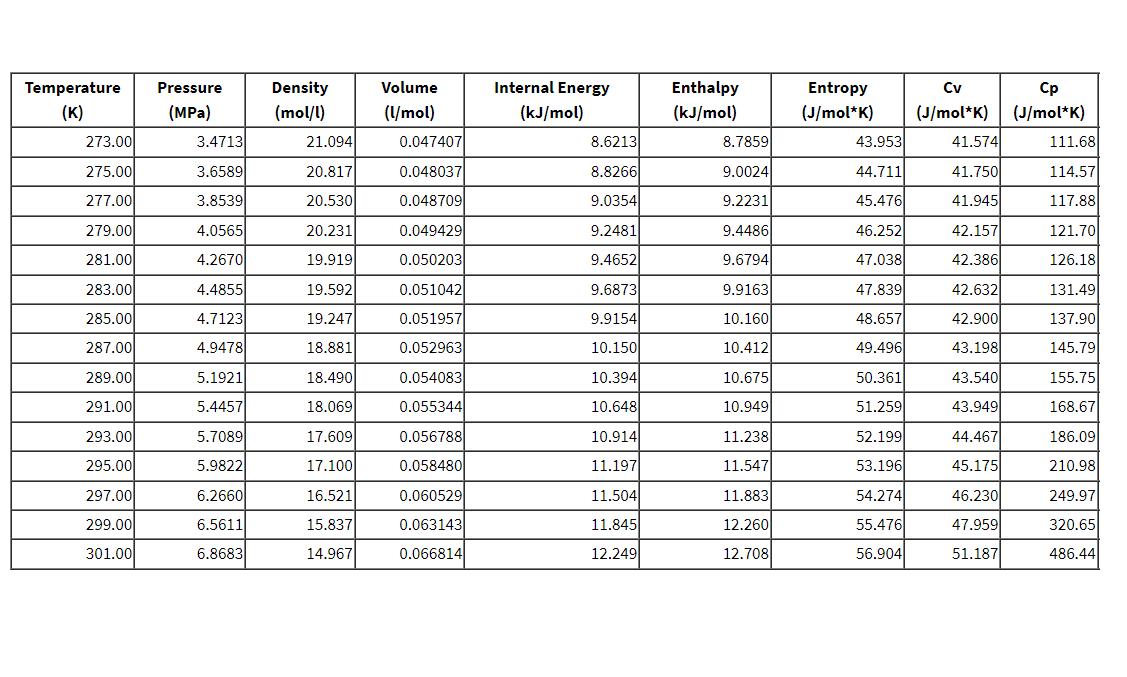
\includegraphics[scale=0.75]{Problem_2/Liquid_phase.png}
    
%     \label{fig:enter-label}
% \end{figure}

\begin{center}
\footnotesize{
\begin{tabular}{|>{\centering\arraybackslash}m{2cm}|>{\centering\arraybackslash}m{2cm}|>{\centering\arraybackslash}m{2cm}|>{\centering\arraybackslash}m{2cm}|>{\centering\arraybackslash}m{2cm}|>{\centering\arraybackslash}m{2cm}|}
    \hline
    Nhiệt độ & Áp suất & Mật độ mol & Nội năng & Enthalpy & Entropy \\
    $(\si{K})$ & $(\si{MPa})$ & $(\si{mol/l})$ & $(\si{kJ/mol})$ & $(\si{J/mol \cdot K})$ & $(\si{J/mol \cdot K})$ \\
    \hline
    273.00 & 3.4713 & 21.094 & 8.6213 & 8.7859 & 43.953 \\
    \hline
    275.00 & 3.6589 & 20.817 & 8.8266 & 9.0024 & 44.711 \\
    \hline
    277.00 & 3.8539 & 20.530 & 9.0354 & 9.2231 & 45.476 \\
    \hline
    279.00 & 4.0565 & 20.231 & 9.2481 & 9.4486 & 46.252 \\
    \hline
    281.00 & 4.2670 & 19.919 & 9.4652 & 9.6794 & 47.038 \\
    \hline
    283.00 & 4.4855 & 19.592 & 9.6873 & 9.9163 & 47.839 \\
    \hline
    285.00 & 4.7123 & 19.247 & 9.9154 & 10.160 & 48.657 \\
    \hline
    287.00 & 4.9478 & 18.881 & 10.150 & 10.412 & 49.496 \\
    \hline
    289.00 & 5.2921 & 18.490 & 10.394 & 10.675 & 50.361 \\
    \hline
    291.00 & 5.4457 & 18.069 & 10.648 & 10.949 & 51.259 \\
    \hline
    293.00 & 5.7089 & 17.609 & 10.914 & 11.238 & 52.199 \\
    \hline
    295.00 & 5.9822 & 17.100 & 11.197 & 11.547 & 53.196 \\
    \hline
    297.00 & 6.2660 & 16.521 & 11.504 & 11.883 & 54.274 \\
    \hline
    299.00 & 6.5611 & 15.837 & 11.845 & 12.260 & 55.476 \\
    \hline
    301.00 & 6.8683 & 14.967 & 12.249 & 12.708 & 56.904 \\
    \hline
\end{tabular}
}
\end{center}

\begin{flushright}
    (Biên soạn bởi Yuki)
\end{flushright}
\setcounter{equation}{0}
\begin{center}
    \normalcolor{\textbf{Bài giải}}
\end{center}
\begin{enumerate}[label=\textbf{\alph*,}]\itemsep0em
\item Theo nguyên lý 1 nhiệt động lực học:
\begin{equation} \label{eq1_P2_d1}
    T dS = dU + pdV.
\end{equation}
Ta nhớ rằng nội năng khí lý tưởng tuân theo biểu thức:
\begin{equation} \label{eq2_P2_d1}
    dU = C_V dT = \frac{R}{\gamma-1} dT.
\end{equation}
Phương trình Clapeyron-Mendeleev cho $\SI{1}{mol}$ khí lý tưởng: 
\begin{equation} \label{eq3_P2_d1}
    p=\frac{RT}{V}.
\end{equation}
Thay các phương trình (\ref{eq2_P2_d1}) và (\ref{eq3_P2_d1}) vào phương trình (\ref{eq1_P2_d1}) rồi chia hai vế cho $T$, ta được
\begin{equation} \label{eq4_P2_d1}
    dS = \frac{R}{\gamma-1} \frac{dT}{T} + R \frac{dV}{V}.
\end{equation}
Lấy nguyên hàm phương trình (\ref{eq4_P2_d1}), ta thu được hàm entropy của khối khí là một hàm trạng thái chỉ phụ thuộc vào $T$ và $V$:
\begin{equation} \label{eq5_P2_d1}
    S(T,V)= \frac{R}{\gamma-1} \ln (T) + R \ln (V) + S_0.
\end{equation}
Với $S_0$ là một hằng số.

\item Ta biết rằng, các quá trình đoạn nhiệt là các quá trình đẳng entropy (entropy không đổi), chúng sẽ là những đường thẳng đứng vuông góc với trục hoành trên đồ giản đồ $T$-$S$. Còn các quá trình đẳng nhiệt sẽ là các đường nằm ngang vuông góc với trục tung $T$, mỗi đường giãn đẳng nhiệt làm thể tích tăng $n_i$ lần được biểu diễn trên giản đồ $T$-$S$ này, theo biểu thức (\ref{eq5_P2_d1} sẽ ứng với một đoạn có độ dài $\Delta S_i = R \ln (n_i)$. Như vậy ta thu được đồ thị:

\begin{center}
\begin{tikzpicture}[>=stealth]
    %Vẽ hệ trục toạ độ 
    \draw[->](0,2.0)--(13,2.0);
    \draw[->](0,2.0)--(0,8.0);
    \draw (13,2) node[above]{$S$} (0,8.0) node[left]{$T$} (0,2.0) 
    node[below left]{$O$};
    %Vẽ đồ thị
    \draw[->] (3,7.0)--(4,7.0);
    \draw[->] (4,7.0)--(4,6.5);
    \draw[->] (4,6.5)--(5,6.5);
    \draw[->] (5,6.5)--(5,6.0);
    \draw[->] (5,6.0)--(6,6.0);
    \draw[->] (6,6.0)--(6,5.5);
    \draw[->] (6,5.5)--(7,5.5);
    \draw[->] (7,5.5)--(7,5.0);
    \draw[->] (7,5.0)--(8,5.0);
    \draw[->] (8,5.0)--(8,4.5);
    \draw[->] (8,4.5)--(9,4.5);
    \draw[->] (9,4.5)--(9,4.0);
    \draw[->] (9,4.0)--(10,4.0);
    \draw[->] (10,4.0)--(10,3.5);
    \draw[->] (10,3.5)--(3,3.5);
    \draw[->] (3,3.5)--(3,7.0);
    %Nhiệt độ 
    \draw (3.5,7.0) node[above]{$T_1$};
    \draw (4.5,6.5) node[above]{$T_2$};
    \draw (5.5,6.0) node[above]{$T_3$};
    \draw (6.5,5.5) node[above]{$T_4$};
    \draw (7.5,5.0) node[above]{$T_5$};
    \draw (8.5,4.5) node[above]{$T_6$};
    \draw (9.5,4.0) node[above]{$T_7$};
    \draw (6.5,3.5) node[above]{$T_8$};
    %Ghi chú \Delta S.
    \draw[dashed] (7,5.0)--(7,2.0);
    \draw[dashed] (8,5.0)--(8,2.0);
    \draw (7.5,2.0) node[below]{$\Delta S_i = R \ln (n_i)$};
\end{tikzpicture}
\end{center}


\item Ta có thể xác định được hiệu entropy giữa điểm đầu và điểm cuối của quá trình nén đẳng nhiệt thông qua 2 con đường của đồ thị. Gọi tỷ số thể tích giữa trạng thái đầu và trạng thái cuối của quá trình nén đẳng nhiệt là $n_8$. Ta có thể xác định được hiệu entropy giữa điểm đầu và điểm cuối của quá trình co đẳng nhiệt thông qua 2 con đường của đồ thị:
\begin{equation} \label{eq6_P2_d1}
    \begin{split}
        & R \ln (n_1) + R \ln (n_2) + ... + R \ln (n_6) + R \ln (n_7) = R \ln (n_8) \ \ \ (= \Delta S_8) \\
        & \Rightarrow n_8 = n_1 n_2 n_3 n_4 n_5 n_6 n_7 \approx 1.60.
    \end{split}
\end{equation}

\item Việc tính công của chu trình này thông qua việc tính tổng công của từng quá trình nhỏ tương đối phức tạp. Song, ta hoàn toàn có thể thay thế công việc này thông qua tính tổng nhiệt lượng khí nhận nhiệt $Q_1$ và tống nhiệt lượng khí nhả ra $Q_2$ rồi xác định công của khối khí thực hiện là $W'=Q_1-Q_2$.

Theo định nghĩa của entropy nhiệt động lực học, ta dễ dàng có thể lấy nó ở dạng tích phân trong trường hợp này:
\begin{equation} \label{eq7_P2_d1}
    Q = \sum T_i \Delta S_i.
\end{equation}
Áp dụng công thức trên, ta tìm được:
\begin{equation} \label{eq8_P2_d1}
    Q_1 = T_1 R \ln (n_1) + T_2 R \ln (n_2) + T_3 R \ln (n_3) +...+ T_6 R \ln (n_6) + T_7 R \ln (n_7).
\end{equation}
Và 
\begin{equation} \label{eq9_P2_d1}
    Q_2 = T_8 R \left[ \ln (n_1) + \ln (n_2) + \ln (n_3) +...+ \ln(n_6) + \ln (n_7)  \right].
\end{equation}
Vậy công khí thực hiện trong quá trình là:
\begin{equation} \label{eq10_P2_d1}
    W'= Q_1 - Q_2 = \sum_{i=1}^7 R \left( T_i - T_8 \right) \ln (n_i) = \SI{179}{J}.
\end{equation}
Hiệu suất của chu trình:
\begin{equation} \label{eq11_P2_d1}
    H = 1 - \frac{Q_2}{Q_1} = 1 - \frac{\displaystyle T_8 \sum_{i=1}^7 \ln (n_1)}{\displaystyle \sum_{i=1}^7 T_i \ln (n_i)} = 13.1 \%.
\end{equation}

\end{enumerate}

\textbf{Biểu điểm} 
\begin{center}
\begin{tabular}{|>{\centering\arraybackslash}m{1cm}|>{\raggedright\arraybackslash}m{14cm}| >{\centering\arraybackslash}m{1cm}|}
    \hline
\textbf{Phần} & \textbf{Nội dung} & \textbf{Điểm} \\
    \hline
    \textbf{a} & Tìm được hàm entropy $S(T,V)$ (\ref{eq5_P2_d1}) & $0.50$ \\
    \hline
    \textbf{b} & Vẽ phác đồ thị & $1.00$ \\
    \hline
    \textbf{c} & Tính được $n_8$ (\ref{eq6_P2_d1}) & $1.00$ \\
    \hline
    \textbf{d} & Tính $Q_1$ (\ref{eq8_P2_d1}) & $0.50$ \\
    \cline{2-3}
    & Tính công $W'$ (\ref{eq10_P2_d1}) & $0.50$ \\ 
    \cline{2-3}
    & Tính hiệu suất $H$ (\ref{eq11_P2_d1}) & $0.50$ \\
    \hline
\end{tabular}
\end{center}

\noindent \textbf{Mở rộng vấn đề:} \\
Đây là một bài toán lấy ý tưởng từ bài 2 ngày 1 VPhO 2022 (một bài toán cũng thường xuất hiện trong các sách bài tập vật lý đại cương). Không khó để nhận thấy, việc mở rộng bài toán từ 3 cặp đường đẳng nhiệt và đoạn nhiệt lên thành 8 cặp đường không phải là chỉ để tăng sự phức tạp trong tính toán mà còn đòi hỏi người giải phải tìm ra được quy luật tổng quát của bài toán với số cặp đường đẳng nhiệt và đoạn nhiệt là bất kì. Phần \textbf{a} và \textbf{b} của bài toán đã được đưa vào với mục đích dẫn dắt đến một lời giải đơn giản hơn so với cách làm thường thấy. \\
Lời giải này đưa đến 2 thủ thuật nho nhỏ:
\begin{enumerate}
    \item Đôi khi entropy cho phép ta đơn giản hoá các vấn đề trong tính toán (đặc biệt là trong các bài toán có các quá trình đẳng nhiệt và đoạn nhiệt).
    \item Đôi khi, việc tính công của quá trình trở nên phức tạp hơn việc xác tìm nhiệt lượng thu $Q_1$ và nhiệt lượng toả $Q_2$.
\end{enumerate}
Hiển nhiên, các thủ thuật kia chỉ có thể dùng từ "đôi khi", khá nhiều khi chúng phản tác dụng và việc sử dụng chúng hiệu quả không sẽ phụ thuộc vào kinh nghiệm của người giải. Cho một số ứng dụng đơn giản, hãy thử những mẹo trên và mở rộng bài toán này cho $p$ quá trình giãn và $q$ quá trình co, giải lại các bài toán về chu trình Carnot, chu trình Otto, chu trình Atkinson, chu trình Stirling,... chúng có thể không mang đến một lời giải hoàn hảo như ở bài toán này, song chúng vẫn có những hiệu quả nhất định khi sử dụng.

Đây chỉ là một bài toán mang tính giáo dục cũng như đưa ra các cách giải quyết vấn đề thú vị chưa được sử dụng nhiều trong các tài liệu Olympiad, các số liệu trong bài toán chỉ nhằm mục đích kiểm tra đáp số đơn giản hơn, không có ý nghĩa thực tế.


\newpage
{\normalcolor \textbf{CÂU 3 (4 điểm)}}\vspace{1.5mm}

\setcounter{equation}{0}
% \textbf{Định lý Earnshaw và thấu kính tĩnh điện}

% Một vòng dây điện tích \(Q\) hình đa giác đều \(n\) cạnh có bán kính đường tròn ngoại tiếp \(R\). Trục \(\Delta\) là trục đi qua tâm và vuông góc với mặt phẳng vòng dây có dạng đối xứng trụ.

% \ \ 

% \textbf{1.} Chứng minh rằng, điện trường ở gần trục \(\Delta\).

% \ \ 

% \textbf{2.} Tính vector điện trường \(\mathbf{E}\) tại một vị trí gần trục \(\Delta\).

% \ \ 

% Theo định lý Earnshaw, một hệ điện tích trong chân không không thể tạo ra một điểm cân bằng bền chỉ bởi các tương tác tĩnh điện.

% \ \  

% \textbf{3.} Chỉ ra rằng trong bài toán này, vị trí cân bằng không thể là vị trí cân bằng bền với mọi chuyển động.

% \ \ 

% \textbf{4.} Bắn một hạt điện tích \(q\) khối lượng \(m\) với vận tốc \(v_0\) song song với trục \(\Delta\) và cách trục \(\Delta\) một khoảng \(b\) (với \(b \ll R\) ). Quỹ đạo của hạt điện tích đi qua vòng dây điện tích giống như một tia sáng đi qua thấu kính có tiêu cự \(f\). Tính tiêu cự \(f\) này theo \(n\), \(R\), \(Q\), \(q\), \(\varepsilon_0\), \(m\) và \(v_0\).

\textbf{Hiệu ứng bề mặt} \footnote{Skin effect.}

Hiệu ứng bề mặt là một hiệu ứng xuất hiện phổ biến trong các các đường mạch điện truyền dẫn dòng điện cao tần. Theo đó, thay vì phân bố đều trên toàn dây dẫn như các dòng điện tần số thấp, ở tần số cao, các dòng điện tập trung chủ yếu ở sát bề mặt kim loại và nhanh chóng giảm theo độ sâu với cấp số mũ.

\ \

\textbf{1. Mô hình mạch tương đương đơn giản}

Quy luật chuyển động của dòng điện trong một vật dẫn với hằng số điện môi \(\mu\) và điện trở suất \(\rho\) có thể được mô tả bởi một mạch điện tương đương (như hình \ref{fig:Equivalent_circuit_skin_effect}) \footnote{Điện kháng \(L_0\) được sử dụng để mô tả hằng số từ thẩm trong chân không \(\mu_0\) của môi trường ngoài. Ta không cần quan tâm đến nó trong bài toán này}. Ở hình \ref{fig:Equivalent_circuit_skin_effect}A, phân bố dòng điện trong tấm vật liệu được tương đương như một mạch điện vô hạn, theo đó, từng khối chữ nhật có chiều dài \(l\), chiều rộng \(w\) và độ dày \(\Delta z\) (như hình \ref{fig:Conductor}) được tương đương như một mắt mạch tương đương gồm một thành phần cảm kháng \(\Delta L\) và một phần điện dẫn \footnote{Nghịch đảo của điện trở.} \( \Delta G \).

\begin{figure}[!h]
    \centering
    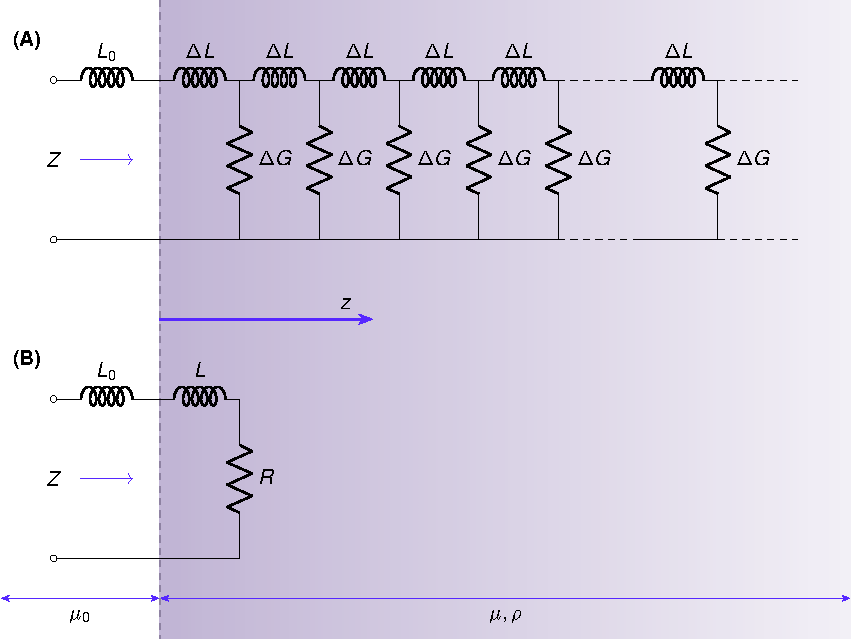
\includegraphics[width=0.9\textwidth]{Problem_3/Figs_P3/Equivalent_circuit_skin_effect.pdf}
    \caption{Mô hình mạch tương đương của hiệu ứng bề mặt. (A) Mạch tương đương phân bố vô hạn trong không gian. (B) Mạch tương đương trở kháng của mạch.}
    \label{fig:Equivalent_circuit_skin_effect}
\end{figure}

Dựa vào các tính toán mạch tương đương, mạng mạch vô hạn tuần hoàn trên có trở kháng quan sát từ phía bề mặt ngăn cách hai môi trường là \(Z\) và có thể được phân tích như tổng của hai phân tử \(R\) và \(L\) (như hình \ref{fig:Equivalent_circuit_skin_effect}B).

\begin{figure}
    \centering
    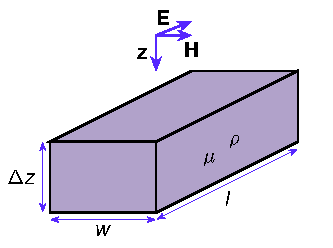
\includegraphics[width=0.6\textwidth]{Problem_3/Figs_P3/Conductor.pdf}
    \caption{Mô hình một phần tử trong khối vật dẫn.}
    \label{fig:Conductor}
\end{figure}

\textbf{Câu hỏi a.} Tìm \( \Delta L \) và \( \Delta G \) của mạch trong mô hình mạch tương đương vô hạn theo \(\mu\), \(\rho\), \(w\), \(l\) và \( \Delta z \).

\ \

\textbf{Câu hỏi b.} Tìm các thông số trở kháng \(Z\), \(R\) và \(L\) theo \(\mu\), \(\rho\), \(w\), \(l\) và tần số \(\omega\) của dòng điện.

\ \

\textbf{Câu hỏi c.} Độ sâu bề mặt\footnote{Skin depth.} là độ sâu để biên độ dòng điện giảm đi \(e\) lần. Xác định độ sâu bề mặt của tấm vật liệu theo tần số \(\omega\) của dòng điện, độ từ thẩm \(\mu\) và điện trở suất \(\rho\).

\ \

\textbf{2. Điện trở gây bởi hiệu ứng bề mặt}

\ \

\textbf{Câu hỏi d.} Chứng minh rằng, ta có thể tính điện trở \(R\) tương đương của một đoạn vật dẫn điện chịu ảnh hưởng bởi hiệu ứng bề mặt có thể tính theo công thức:
\begin{equation}
    R = \dfrac{1}{\mu_0} \dfrac{\partial L_0}{\partial z} R_S,
\end{equation}
trong đó
\begin{itemize}
    \item \(L_0\) là độ tự cảm của một miếng bề mặt vật dẫn được xét với giả thiết độ sâu bề mặt bằng không.
    \item Tọa độ \(z\) được hiểu là tọa độ có trục vuông góc với bề mặt.
    \item \(R_S = \sqrt{\omega \mu \rho/2}\) được gọi là hệ số điện trở suất bề mặt.
\end{itemize}

\ \

\textbf{Câu hỏi e.} Tính điện trở gây ra bởi hiệu ứng bề mặt đối với hai ống dây dẫn tròn có chiều dài \(l\), bán kính \(a\) và có trục dây đặt cách nhau một khoảng \(2b\).
\setcounter{equation}{0}
\begin{center}
    \normalcolor{\textbf{Bài giải}}
\end{center}
\begin{enumerate}[label=\textbf{\alph*,}]\itemsep0em
\item Theo tính đối xứng cầu của hệ, ta có thể dễ dàng suy ra mật độ dòng
\begin{equation} \label{eq1_P3_d1}
    j(r) = \frac{I}{2\pi h r}.
\end{equation}
Một hạt electron chuyển động đến vị trí có bán kính $r$ sẽ nhận được một công $eV(r)$ của điện trường, xem rằng công này được chuyển hoá làm tăng động năng của hạt điện tích $\frac{1}{2}mv^2$, từ đó ta xác định được vận tốc của hạt:
\begin{equation} \label{eq2_P3_d1}
    \frac{1}{2}mv^2 = eV(r) \Rightarrow v(r)= \sqrt{ \frac{2eV(r)}{m} }.
\end{equation}
Theo định nghĩa mật độ dòng:
\begin{equation} \label{eq3_P3_d1}
    j(r) = \rho v \Rightarrow \rho = \frac{j}{v} = \frac{I}{2\pi h r} \sqrt{ \frac{m}{2eV} } .
\end{equation}

\item Trong hệ đối xứng cầu, cường độ điện trường tại bán kính $r$ là
\begin{equation} \label{eq4_P3_d1}
    E = - \frac{dV}{dr}.
\end{equation}
Áp dụng định luật Gauss cho một vỏ trụ bán kính $r$ và độ dày $dr$, ta có
\begin{equation} \label{eq5_P3_d1}
    \begin{split}
        E(r+dr) \cdot 2 \pi h (r+dr) - E(r) \cdot 2 h \pi r &= \frac{\rho}{\varepsilon_0} \cdot 2 \pi h r dr \\
        \Rightarrow \frac{d}{dr} \left( E \cdot r \right) = \frac{\rho}{\varepsilon_0} r.
    \end{split}
\end{equation}
Từ (\ref{eq4_P2_d1}) và (\ref{eq5_P3_d1}), ta được:
\begin{equation} \label{eq6_P3_d1}
    \frac{1}{r} \frac{d}{dr} \left( r \frac{dV}{dr} \right) = \frac{\rho}{\varepsilon_0}.
\end{equation}
\item Từ (\ref{eq3_P2_d1}) và (\ref{eq6_P3_d1}) ta thu được phương trình vi phân của $V(r)$:
\begin{equation} \label{eq7_P3_d1}
    \frac{d}{dr} \left( r \frac{dV}{dr} \right) = \frac{I}{2\pi \varepsilon_0 h} \sqrt{ \frac{m}{2eV} } .
\end{equation}
Thế dạng nghiệm $V(r)=Ar^\alpha$ vào phương trình (\ref{eq7_P3_d1}), ta được:
\begin{equation} \label{eq8_P3_d1}
    A \alpha^2 r^{\alpha-1} = \frac{I}{2 \pi \varepsilon_0 h} \sqrt{ \frac{m}{2e A} } r^{-\alpha/2}.
\end{equation}
Đồng nhất hệ số 2 vế, ta được:
\begin{equation} \label{eq9_P3_d1}
    \alpha-1=-\frac{\alpha}{2} \Rightarrow \alpha = \frac{2}{3}.
\end{equation}
Và 
\begin{equation} \label{eq10_P3_d1}
    A \alpha^2 = \frac{I}{2 \pi \varepsilon_0 h} \sqrt{ \frac{m}{2e A} } \Rightarrow A= \left( \frac{9I}{8\pi \varepsilon_0 h} \sqrt{\frac{m}{2e}} \right)^{2/3}.
\end{equation}
\item Thay (\ref{eq9_P3_d1}) và (\ref{eq10_P3_d1}) vào công thức nghiệm
\begin{equation} \label{eq11_P3_d1}
    V(r) = \left( \frac{9I}{8\pi \varepsilon_0 h} \sqrt{\frac{m}{2e}} \right)^{2/3} r^{2/3}.
\end{equation}
Tại $r=R$ thì $V(R)=U$ nên
\begin{equation} \label{eq12_P3_d1}
    U = \left( \frac{9I}{8\pi \varepsilon_0 h} \sqrt{\frac{m}{2e}} \right)^{2/3} R^{2/3}.
\end{equation}
Hay
\begin{equation} \label{eq13_P3_d1}
    I = \left( \frac{8\pi \varepsilon_0 h}{9R} \sqrt{ \frac{2e}{m} }\right) U^{3/2}.
\end{equation}
Như vậy
\begin{equation} \label{eq14_P3_d1}
    K = \frac{8\pi \varepsilon_0 h}{9R} \sqrt{ \frac{2e}{m} } .
\end{equation}
\end{enumerate}

\textbf{Biểu điểm} 
\begin{center}
\begin{tabular}{|>{\centering\arraybackslash}m{1cm}|>{\raggedright\arraybackslash}m{14cm}| >{\centering\arraybackslash}m{1cm}|}
    \hline
\textbf{Phần} & \textbf{Nội dung} & \textbf{Điểm} \\
    \hline
    \textbf{a} & Tìm được mật độ dòng $j$ theo $I$ (\ref{eq1_P3_d1}) & $0.25$ \\
    \cline{2-3}
    & Tìm vận tốc $v$ theo điện thế $V$ (\ref{eq2_P3_d1}) & $0.50$ \\
    \cline{2-3}
    & Tìm mật độ điện khối $\rho$ theo $V$ và $r$ (\ref{eq3_P3_d1}) & 0.25 \\
    \hline
    \textbf{b} & Viết biểu thức điện trường theo điện thế (\ref{eq4_P3_d1}) & $0.25$ \\
    \cline{2-3}
    & Áp dụng định luật Gauss cho vỏ trụ (\ref{eq5_P3_d1}) & $0.50$ \\
    \cline{2-3}
    & Kết hợp 2 phương trình để viết được phương trình vi phân (\ref{eq6_P3_d1}) & 0.25 \\
    \hline
    \textbf{c} & Hoàn chỉnh phương trình vi phân (\ref{eq7_P3_d1}) & $0.25$ \\
    \cline{2-3}
    & Thế dạng nghiệm của phương trình (\ref{eq8_P3_d1}) & $0.25$ \\
    \cline{2-3}
    & Tính được $\alpha$ (\ref{eq9_P3_d1}) & $0.50$ \\
    \cline{2-3}
    & Tính được $A$ (\ref{eq10_P3_d1}) & $0.50$ \\ 
    \hline
    \textbf{d} & Thay điều kiện biên và viết được $U$ theo $I$ (\ref{eq12_P3_d1}) & $0.25$ \\ 
    \cline{2-3}
    & Tính hệ số $K$ (\ref{eq14_P3_d1}) & $0.25$ \\
    \hline
\end{tabular}
\end{center}

\noindent \textbf{Mở rộng vấn đề:} \\
Đây là một bài toán không có các tính toán phức tạp nhưng khá khó để nhìn được ra đường hướng giải quyết, đòi hỏi người giải cần có một kiến thức nền khá tốt. Đối với những người đã học tương đối sâu về phân bố của điện từ trường và biết sử dụng các công cụ toán tốt, không khó để nhận thấy câu hỏi phần \textbf{b} chính là chứng minh phương trình Poisson $\Delta V = \frac{\rho}{\varepsilon_0}$ đối với hệ toạ độ trụ có tính đối xứng trụ, đây là một phương trình được dẫn ra từ 2 trong 4 phương trình Maxwell, 1 phương trình là định luật Gauss về thông lượng của điện trường và 1 phương trình về lưu số của điện trường (liên hệ giữa điện trường và điện thế). Tổng quát hơn, với mọi bài toán về tĩnh điện và các hệ từ trường dừng, ta sẽ đều cần sử dụng 1 phương trình về thông lượng và 1 phương trình về lưu số để giải quyết chúng. \\
Bài toán diot chân không và định luật Child-Langumuir được lấy từ Bài tập giải sẵn "Diode chân không" trang 59-60 quyển \textit{Điện từ học 2} của Jean Marie Brébec (bộ sách PFIEV), bản dịch của Lê Băng Xương, Nhà xuất bản giáo dục Việt Nam. Bài toán được tham khảo thêm từ bài 2.53 trang 109 trong quyển sách \textit{Introduction to Electrodynamics} của David Griffiths cũng như các bài báo về "Child-Langumuir law". \\
Như ta có thể thấy, bài toán diode chân không này phổ biến nhất là trường hợp 2 bản tụ phẳng rộng có diện tích $S$ đặt song song cách nhau một khoảng $d$ như trong bài 2.53 quyển \textit{Introduction to Electrodynamics}. Kết quả của bài toán này sẽ là:
$$ I = \frac{4 \varepsilon_0 S}{9d^2} \sqrt{ \frac{2e}{m}} U^{3/2}.$$
Các vấn để mở rộng cho bài toán này như khảo sát trường hợp electron có vận tốc ban đầu $v_0$ đáng kể cũng được được xét tới trong các bài báo \href{https://arxiv.org/abs/physics/0411175v1}{Generalization of Child-Langmuir Law for Non-Zero Injection Velocities in a Planar} và \href{http://de.arxiv.org/abs/1506.07417v1}{A new approach to the Child-Langmuir law}. 

Bài toán của chúng ta là dạng hình trụ của diode, tất nhiên, ta hoàn toàn có thể mở rộng bài toán này cho trường hợp hệ diode hình cầu, song nó đưa đến một phương trình vi phân tương đối phức tạp và không phù hợp để giải ở đây.

\newpage
{\normalcolor \textbf{CÂU 4 (4 điểm)}}\vspace{1.5mm}

\setcounter{equation}{0}
\textbf{Khuếch đại thuật toán}

Bộ khuếch đại thuật toán (OPerational AMPlifier), hay còn gọi là OPAMP là một linh kiện điện tử dùng để thực hiện một số phép toán như cộng, trừ, nhân, chia, tích phân, đạo hàm,... khi nó kết hợp với các linh kiện bên ngoài.

Một OPAMP cơ bản có cấu tạo gồm 8 chân, nhưng trong khuôn khổ bài này, chúng ta chỉ xét một OPAMP như hình vẽ


\begin{figure}[h]
\centering
\begin{subfigure}[t]{0.3\textwidth}
\centering
\begin{circuitikz} 
    \draw
     (0,0) node[op amp] (opamp) {}
     (opamp.+) node[left] {$v_+$}
     (opamp.-) node[left] {$v_-$}
     (opamp.out) node[right] {$v_o$}
     (opamp.up) --++(0,0.5) node[vcc]{$V_+$}
     (opamp.down) --++(0,-0.5) node[vee]{$V_-$};
    \end{circuitikz}
 \caption{Ký hiệu OPAMP}
 \end{subfigure}
 %
\begin{subfigure}[t]{0.6\textwidth}
 \centering
 \begin{circuitikz}[american,scale=0.73,font=\footnotesize]
 \ctikzset{bipoles/length=11mm} 
    \draw
        (0,4) to[short, -o] ++(-1.7,0) node[shift={(-0.4,0)}] {$v_-$}
        (-1.7, 3.6) to [short, -*] (-1.7, 3.6) node[ground]{}
        (0,0) to[short, -o] ++(-1.7,0) node[shift={(-0.4,0)}] {$v_+$}
        (-1.7,-0.4) to [short, -*] (-1.7,-0.4) node[ground]{}
        (0,4) to[resistor, l=$R_\text{in}$] (0,0)
        (1.5,0.5) to [short,-*] (1.5,0.5) node[ground]{} to [cV, invert, l_=$A(v_+ - v_-)$] ++(0,1.5) to [resistor, l=$R_\text{out}$] ++(5.5,0) to [short, -o] ++(0.1,0) node[shift={(0.4,0)}] {$v_\text{o}$}
        (-1,-2) to [short] ++(0,8) to [short] (6.5,2) to [short] (-1,-2) 
        (-1.7, 3) node[below,shift={(-0.,0)} ] {$v_G=0$}
    ;\end{circuitikz}
 \caption{Mạch tương đương của OPAMP}\label{opampcircuit}
 \end{subfigure}
 \caption{OPAMP}
 \end{figure}


Trong đó hai chân $V_+$ và $V_-$ dùng để cấp nguồn cho thiết bị, khi có hai điện thế $v_+$ và $v_-$ được đặt lần lượt vào hai đầu vào không đảo ngược và đảo ngược thì ở đầu ra sẽ xuất hiện một điện thế $v_0$ sao cho:
\begin{equation}
    v_0=A(v_+-v_-) \ \ ,
\end{equation}
trong đó A được gọi là "độ lợi vòng lặp hở" đặc trưng với từng loại OPAMP. Thiết bị này có thể được miêu tả bằng mô hình mạch điện \subref{opampcircuit}, trong đó ký hiệu của nguồn $A(v_+ - v_-)$ gọi là nguồn áp phụ thuộc, tức là độ lớn của nó phụ thuộc vào một đại lượng khác(ở đây là hiệu điện thế giữa hai đầu vào của OPAMP). 




Trong thực tế, OPAMP thường được kết hợp với một số linh kiện ngoài như điện trở, tụ điện hoặc cuộn cảm để phản hồi giữa đầu ra và đầu vào, giúp cho chúng ta có thể điều chỉnh được độ lợi của OPAMP bằng cách điều chỉnh các thông số thiết bị ngoài.
\begin{enumerate}
    \item Tìm độ lợi vòng lặp đóng $\dfrac{v_\text{o}}{v_\text{s}}$ cho mạch dưới đây. Áp dụng với LM741 có độ lợi vòng lặp mở $2 \times 10^5$, điện trở đầu vào $2 \si{M\Omega}$ và điện trở đầu ra $50 \si{\Omega}$ và $R_f=200 \si{\Omega}$, $R_1=100 \si{\Omega}$.
\end{enumerate}
\begin{center}
    \begin{circuitikz}[american]\draw
(0,0) node[op amp] (opamp) {}
 (opamp.+)  to [short] ++ (-1.5,0) to [short] ++(0,-2) node[ground]{} 
 (opamp.-) to [R,l_={$R_1$},i_<=$i_1$] ++(-3,0) to [V, l_=$v_\text{s}$] ++(0,-3) to [short,-o] ++(6,0) node[right]{$-$}
 (opamp.out) to [short,-o] ++(0.62,0) node[right] {$+$}
 (1.64,-1.3) node[right]{$v_o$}
 (opamp.-) to [short]++(-0.5,0) to [short] ++(0,1) to [R,l={$R_f$},i>=$i_f$] ++(2.9,0) to (opamp.out)
 (opamp.-) node[above left]{I}
 (opamp.out) node[above right]{O}
;\end{circuitikz}
\end{center}

Tiếp theo đây, để cho đơn giản, ta coi các OPAMP là lý tưởng, nghĩa là điện trở đầu vào rất lớn, điện trở đầu ra rất nhỏ và độ lợi vòng lặp hở rất lớn. Khi đó $v_1 \approx v_2$ và dòng điện ở hai đầu vào OPAMP $i_-=i_+=0$.
\begin{enumerate}[resume]
    \item Tìm tỉ số $\dfrac{v_o}{v_s}$ với mạch trên khi OPAMP là lý tưởng.    
\end{enumerate}
Xét ba mạch OPAMP có dạng như hình vẽ:
\begin{figure}[h]
\begin{subfigure}[t]{0.6\textwidth}
\centering
\begin{circuitikz}[american,scale=1]
\draw
(-2,0) node[op amp] (opamp) {}
 (opamp.+) to [short] ++ (-1.5,0) to [short] ++(0,-2) node[ground]{} 
 (opamp.-) to [short] ++(-4.5,0) to[R,l_={$R_2$}] ++(0,-1.5)to [V, l_=$v_\text{2}$] ++(0,-1.5)
 (opamp.-) to [short] ++(-3,0) to[R,l_={$R_1$}] ++(0,-1.5)to [V, l_=$v_\text{1}$] ++(0,-1.5)
 (opamp.-) to [short] ++(-6,0) to[R,l_={$R_3$}] ++(0,-1.5)to [V, l_=$v_\text{3}$] ++(0,-1.5) to [short,-o] ++(9,0) node[right]{$-$}
 (opamp.out) to [short,-o] ++(0.62,0) node[right] {$+$}
 (-0.5,-1.3) node[]{$v_\text{sum}$}
 (opamp.-) to [short] ++(0,1) to [R,l={$R_f$},i>=$i_f$] ++(2.4,0) to (opamp.out)
;\end{circuitikz}
 \caption{Mạch cộng}
 \end{subfigure}
 %
\begin{subfigure}[t]{0.4\textwidth}
 \centering
 \begin{circuitikz}[american,font=\small]\draw
(0,0) node[op amp] (opamp) {}
 (opamp.+) to [short] ++ (-1.5,0) to [V,l=$v_s$] ++(0,-2) node[ground]{} 
 (opamp.-) to [R,l_={$R$}] ++(-3,0) to [short] ++(0,-3) to [short,-o] ++(6,0) node[right]{$-$}
 (opamp.out) to [short,-o] ++(0.62,0) node[right] {$+$}
 (1.64,-1.3) node[right]{$v_\text{ni}$}
 (opamp.-) to [short] ++(0,1) to [R,l={$R_f$},i>=$i_f$] ++(2.4,0) to (opamp.out)
 ;\end{circuitikz}
 \caption{Mạch khuếch đại không đảo}
 \end{subfigure}\\[1ex]
\begin{subfigure}{\linewidth}  
\centering
 \begin{circuitikz}[american]\draw
(0,0) node[op amp] (opamp) {}
 (opamp.+) to [short] ++ (-1.5,0) to [short] ++(0,-2) node[ground]{} 
 (opamp.-) to [R,l_={$R$}] ++(-3,0) to [V, l=$v_\text{s}$] ++(0,-3) to [short,-o] ++(6,0) node[right]{$-$}
 (opamp.out) to [short,-o] ++(0.62,0) node[right] {$+$}
 (1.64,-1.3) node[right]{$v_\text{int}$}
 (opamp.-) to [short] ++(0,1) to [C,l={$C$},i>=$i_f$] ++(2.4,0) to (opamp.out)
  ;\end{circuitikz}
 \caption{Mạch tích phân}
 \end{subfigure}
 \end{figure}

\begin{enumerate}[resume]
    \item Tìm $v_\text{sum}$ ,$v_\text{int}$ và $v_\text{ni}$ ứng với ba mạch.
    \item Từ các mạch trên, thiết lập mạch điện để giải phương trình vi phân sau:
    \begin{equation}
        a\dfrac{d^2x}{dt^2}+b\dfrac{dx}{dt}+cx=d ,
    \end{equation}
với điều kiện ban đầu $\dot{x}(0)=e$, $x(0)=f$ .
    \item Đề xuất một cách thiết kế để tạo ra một phần tử mạch điện có giá trị "điện trở âm" ($V_{in}/I_{in} < 0$) bằng các điện trở, OPAMP và nối đất.  
\end{enumerate}

\begin{flushright}
    (Biên soạn bởi Hiagari)
\end{flushright}


\setcounter{equation}{0}
\begin{center}
    \normalcolor{\textbf{Bài giải}}
\end{center}
\textbf{1.} \textbf{a,} Sơ đồ tạo ảnh:
\begin{align}
     S_1 \xrightarrow[\displaystyle \infty \quad F]{\displaystyle F} S_2 \xrightarrow[\displaystyle L -F \quad l- f]{\displaystyle f_0} S_3 \xrightarrow[\displaystyle  f \quad \infty]{\displaystyle f} S_4.
\end{align}


Ta có phương trình tạo ảnh của thấu kính trường là
\begin{align}
\frac{1}{f_0} &= \frac{1}{L - F} + \frac{1}{d_0 - f}\\
\Leftrightarrow L &= F + \frac{f_0 (l - f)}{l - f - f_0} = 1177.5 \mathrm{~mm}.\label{41}
\end{align}

\textbf{b,} Độ bội giác của hệ ba thấu kính là
\begin{align}
    G_\infty = \frac{F}{f} \frac{l - f}{L - F} = \frac{F}{f} \left( 1 + \frac{f-l}{f_0} \right)  = \frac{160}{3} \approx 53.33.
\end{align}

\textbf{2.} Ta có sơ đồ tạo ảnh của \textit{vật kính} qua hệ thị kính:
\begin{align}
     S_1 \xrightarrow[\displaystyle L \quad d']{\displaystyle f_0} S_2 \xrightarrow[\displaystyle l - d' \quad \Delta]{\displaystyle  f} S_3.
\end{align}

Ta có hệ phương trình thấu kính:
\begin{align}
    \frac{1}{f_0} &= \frac{1}{L} + \frac{1}{d'}.\\
    \frac{1}{f} &= \frac{1}{l - d'} + \frac{1}{\Delta}.
\end{align}

Kết hợp với phương trình (\ref{41}) và giải hệ ba phương trình ta thu được kết quả
\begin{align}
    \Delta = f \left[\frac{1}{1 + \dfrac{f}{f_0 - l}} + \frac{f}{F} \frac{1}{\left(1 + \dfrac{f-l}{f_0} \right)^2} \right] =\frac{507}{64} \approx 7.92 \mathrm{~mm}.
\end{align}

Đường kính vòng tròn ánh sáng xuất hiện trên đồng tử mắt người là
\begin{align}
    \delta = -\frac{D}{G_\infty} = -\frac{39}{16} = -2.4375 \mathrm{mm}.
\end{align}

Ta thấy rằng $\delta$ bé hơn kích thước đồng tử mắt người, nên người có thể nhìn được toàn bộ ánh sáng qua hệ.

\vspace{1mm}

\textbf{3.} Để xác định thị trường qua kính thiên văn, ta coi mắt người là nguồn sáng điểm rồi tìm ảnh của mắt qua hệ thấu kính. Ta có sơ đồ tạo ảnh
\begin{align}
     S_1 \xrightarrow[\displaystyle \Delta \quad d_1]{\displaystyle f} S_2 \xrightarrow[\displaystyle l - d_1 \quad d_2]{\displaystyle f_0} S_3 \xrightarrow[\displaystyle  L - d_2 \quad d_3]{\displaystyle F} S_4.
\end{align}
Ta có hệ phương trình thấu kính
\begin{align}
    \frac{1}{f} &= \frac{1}{\Delta} + \frac{1}{d_1}.\\
    \frac{1}{f_0} &= \frac{1}{l - d_1} + \frac{1}{d_2}.\\
    \frac{1}{F} &= \frac{1}{L - d_2} + \frac{1}{d_3}.
\end{align}
Bấm máy thay số liệu ta thu được
\begin{align}
    d_1 &= -7.5\mathrm{~mm}\\
    d_2 &= -225 \mathrm{~mm}\\
    d_3 &=8311.11 \mathrm{~mm}
\end{align}

Giả sử từ mắt nhìn qua được toàn bộ thấu kính mắt. Khi đó đường kính vòng tròn nhìn được trên kính trường là $d_0'$, khi đó
\begin{align}
    \Big| \frac{d_1}{l -d_1} \Big| &= \frac{d}{d_0'}\\
    \Rightarrow d_0' &= 75 \mathrm{~mm} > d_0 = 30 \mathrm{~mm}
\end{align}

Nhận thấy rằng mắt người không thể nhận toàn bộ ánh sáng qua kính mắt.

Làm tương tự đối với kính trường, ta tìm được vòng tròn ánh sáng trên vật kính, gọi là $D'$, khi đó
\begin{align}
    \Big|\frac{d_2}{L - d_2} \Big| &= \frac{d_0}{D'}\\
    \Rightarrow D' &= 187 \mathrm{~mm} > D =130 \mathrm{mm}
\end{align}

Từ đó ta nhận định rằng ánh sáng đi qua toàn bộ vật kính sẽ không bị mất mát năng lượng khi đi đến mắt người, và \textit{không ngược lại}.

\vspace{1mm}
Từ đó ta tìm được góc mở thị trường khi nhìn qua kính thiên văn là 
\begin{align}
    \theta \approx \frac{D}{d_3} = 0.01564\mathrm{~rad}.
\end{align}
Đường kính góc của Mặt Trăng khi nhìn từ Trái Đất là 
\begin{align}
    \theta_M = \frac{2R_M}{d_{ME}} = 0.00900 \mathrm{~rad}.
\end{align}
Cuối cùng, ta xác định được tỉ lệ diện tích của Mặt Trăng so với trường nhìn qua kính thiên văn là
\begin{align}
    k = \left( \frac{\theta_M}{\theta} \right)^2 = 33.4 \%.
\end{align}



 \textbf{Biểu điểm} 
\begin{center}
\begin{tabular}{|>{\centering\arraybackslash}m{1cm}|>{\raggedright\arraybackslash}m{14cm}| >{\centering\arraybackslash}m{1cm}|}
    \hline
    \textbf{Phần} & \textbf{Nội dung} & \textbf{Điểm} \\
    \hline
    \textbf{a} & Viết được biểu thức chữ và giá trị số của $L$ & 0.50\\   
    \cline{2-3}
    &  Viết được biểu thức chữ và giá trị số của $G_\infty$& 0.50\\
    \hline
    \textbf{b} & Tìm được biểu thức chữ và giá trị của $\Delta$ & 1.00 \\
        \cline{2-3}
        & Tìm được $\delta$ & 0.50 \\
    \hline
    \textbf{c} & Tìm được $d_1,d_2,d_3$ & 0.50\\
    \cline{2-3}
    & Chứng minh được toàn bộ ánh sáng qua vật kính khi đến mắt không bị mất mát & 0.50\\
    \cline{2-3}
    & Tìm được tỉ số $k$ & 0.50\\
    \hline
\end{tabular}
\end{center}

\newpage
{\normalcolor \textbf{CÂU 5 (4 điểm)}}\vspace{1.5mm}

\setcounter{equation}{0}
\textbf{Nguyên lý Cực đại Entropy và Đàn chim Bay}

Vật lý hiện diện trong thế giới quanh ta, giúp mô tả các hành vi quần thể của những hệ thống tương tác phức tạp, từ đám khí lý tưởng đến đám đông người. Trong bài tập này, chúng ta sẽ cùng khám phá xem nguyên lý cực đại entropy đã được áp dụng như thế nào để thành lập lên một trong những lý thuyết Vật Lý Sinh thành công nhất hiện đại dùng để mô tả đàn chim bay (xem hình \ref{fig:Bird}A).

\begin{figure}[!h]
    \centering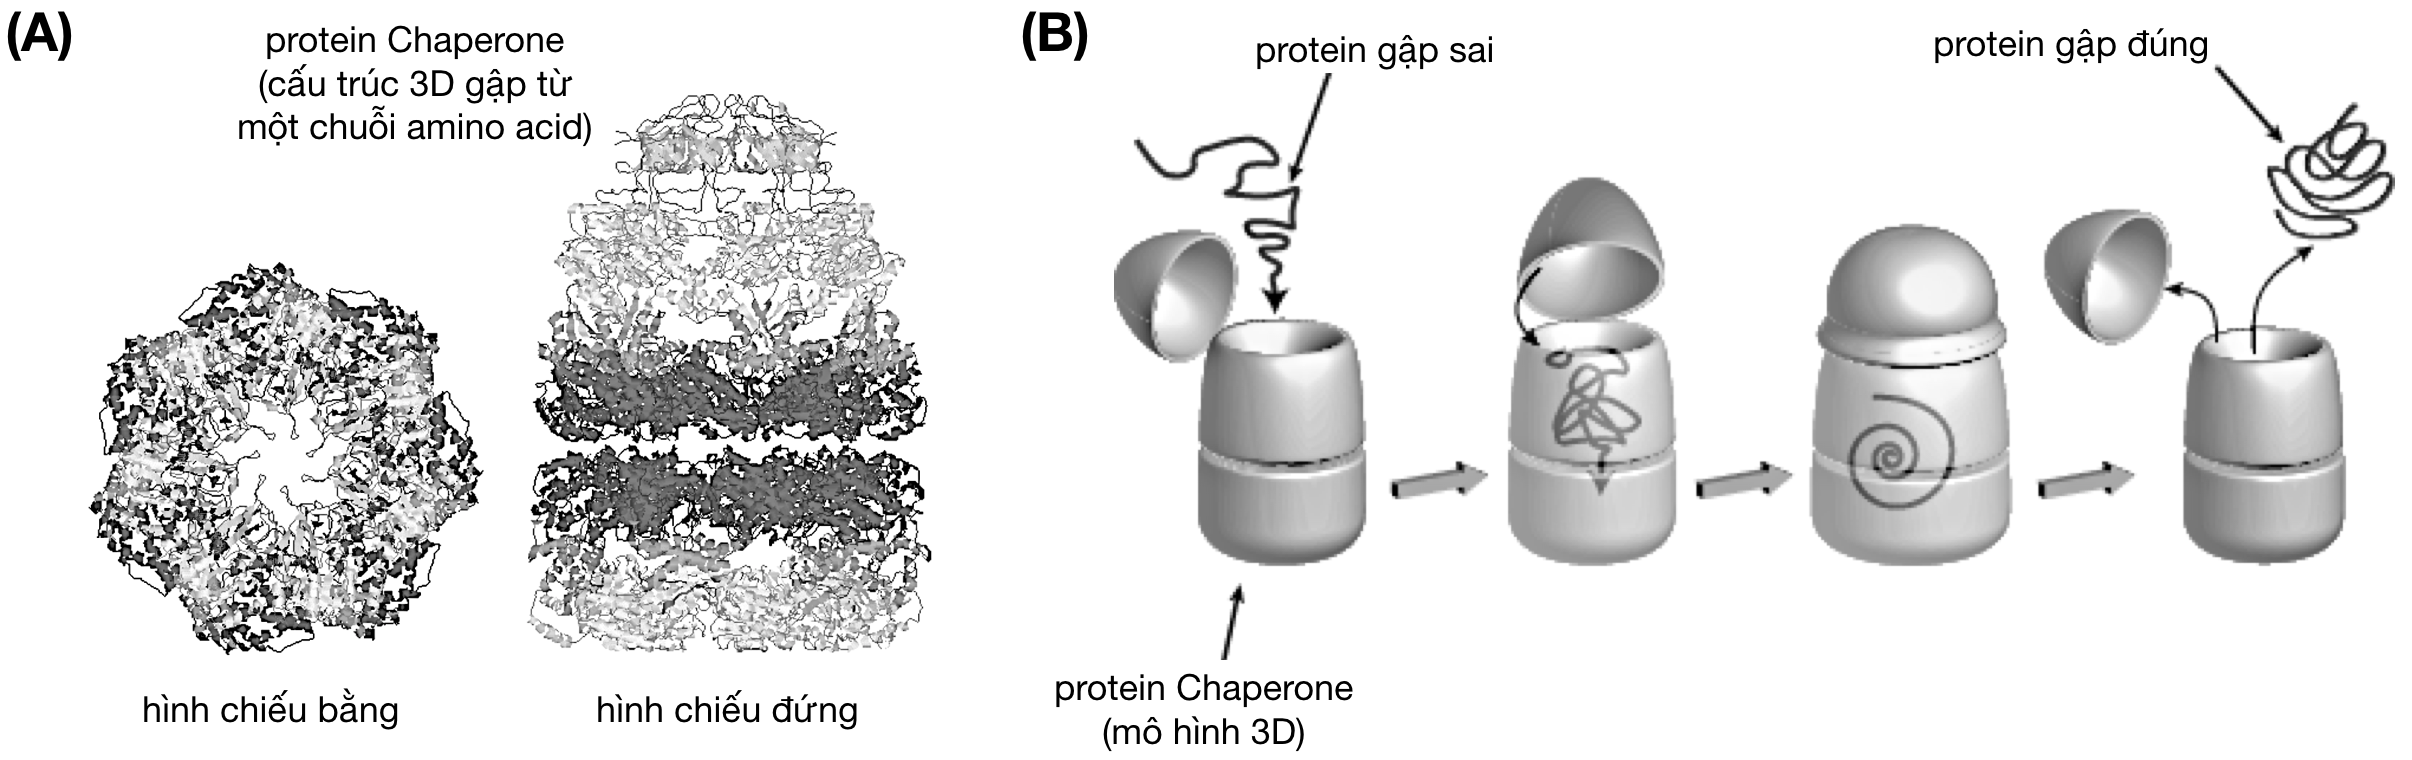
\includegraphics[width=0.96\textwidth]{Problem_5/Figs_P5/fig01.png}
    \caption{(A) Đàn chim bay. (B) Mô tả Toán học của một đàn chim bay, với (B1) là hình ảnh thô của đàn chim và (B2) là tập hợp các vector hướng bay của các cá thể trong đàn chim tại cùng thời điểm.}
    \label{fig:Bird}
\end{figure}

Nguyên lý cực đại entropy là một phương pháp thống kê dùng để suy ra phân phối xác suất không thiên vị nhất có thể dựa trên thông tin đã biết, đồng thời tránh đưa ra giả định về những điều chưa biết. Về cơ bản, nguyên lý này nói rằng, với một tập hợp các ràng buộc đã biết (như giá trị trung bình), phân phối xác suất tốt nhất là phân phối có entropy cao nhất mà vẫn thỏa mãn các ràng buộc này. Ở đây, công thức entropy thường được sử dụng là Boltzmann-Gibbs-Shannon entropy.

\ \ 

Với xác suất xảy ra của một đại lượng Vật Lý liên tục $X$, Boltzmann-Gibbs-Shannon entropy $S$ được xác định bởi giá trị trung bình của hàm \textit{độ ngạc nhiên} $I(x)=-\ln\left[ p(x)\right]$ theo biến $x$:
\begin{equation}
    S = \langle I \rangle = - \int_{\Omega_X} dx \ p(x) \ln\left[ p(x)\right] \ ,
\end{equation}
trong đó $x$ đại diện cho kết quả đo của đại lượng $X$, $p(x)$ là xác suất đo đại lượng $X$ cho ra kết quả $x$,  $\Omega_X$ là vùng khả dĩ của các kết quả đo cho đại lượng $X$.

\ \  

Chúng ta sẽ cùng nhau tìm hiểu về những ứng dụng của nguyên lý này trong việc diễn giải các kết quả thí nghiệm Vật lý, khi trong báo cáo chỉ cung cấp ít các thông tin liên quan.

\ \  

\textbf{1. Phương pháp nhân Lagrange}

Trước hết, chúng ta cùng nhau tìm hiểu về một phương pháp Toán học, vô cùng mạnh mẽ và hiệu quả, giúp chúng ta giải quyết các vấn đề tìm kiếm quỹ tích các điểm cực trị trong bối cảnh có ràng buộc -- phương pháp nhân Lagrange.

\ \ 

Xét việc tìm cực trị của hàm số $f(\vec{z})$ theo biến $\vec{z}\equiv [z_1, z_2, ..., z_{n_z}]$ (trong đó $n_z$ là số lượng các biến), với các điều kiện ràng buộc $C_k(\vec{z})$=0 (trong đó $k=1,2,...,n_C$, và $n_C$ là số lượng điều kiện ràng buộc). Hàm Lagrangian có thể được thiết lập như sau:
\begin{equation}
    L(\vec{Z}) = f(\vec{z}) - \sum_{k=1}^{n_C} \lambda_k C_k(\vec{z}) \ ,
\end{equation}
với biến $\vec{Z} \equiv [\vec{z}, \lambda_1, \lambda_2, \lambda_3, ..., \lambda_{n_C}]$.

\ \ 

\textbf{Câu hỏi a.} Hãy chứng minh rằng, điều kiện cực trị của hàm số $L(\vec{Z})$ theo biến $\vec{Z}$ có thể giúp chúng ta xác định được quỹ tích các điểm cực trị $\vec{z}$ của hàm số $f(\vec{z})$ dưới các ràng buộc $C_k(\vec{z})$.

\ \  

Những câu hỏi tiếp theo đây đều có thể được giải quyết sử dụng phương pháp nhân Lagrange.

\ \  

\textbf{2. Các hàm phân bố nội suy}

Để tránh rườm rà, nhiều báo cáo kết quả thí nghiệm thường không cung cấp toàn bộ dữ liệu thô từ các phép đo, mà chỉ trình bày giá trị ước lượng tốt nhất cùng với độ phân tán của các kết quả, thể hiện qua giá trị trung bình và phương sai.

\ \  

Hãy xác định hàm phân bố nội suy $p(x)$ cho xác suất thu được kết quả $x$ khi đo đại lượng $X$ thỏa mãn nguyên lý cực đại entropy, khi chúng ta chỉ biết những tính chất sau đây:

\ \  

\textbf{Câu hỏi b.} Vùng khả dĩ $\Omega_X$ là miền số thực i.e. $x\in (-\infty,\infty)$, giá trị đo trung bình của $X$ là $\mu$ và giá trị phương sai của $X$ là $\sigma^2 > 0$. Biểu diễn $p(x)$ theo $\mu$, $\sigma^2$, và biến $x$.

\ \  

\textbf{Câu hỏi c.} Vùng khả dĩ $\Omega_X$ là miền số dương i.e. $x\in[0,\infty)$, và giá trị đo trung bình của $X$ là $\mu$ (với $\mu > 0$). Biểu diễn $p(x)$ theo $\mu$ và biến $x$.

\ \  

Bây giờ, chúng ta sẽ áp dụng những kiến thức này vào một hệ vật lý cụ thể. Xét một quần thể gồm nhiều bậc tự do khác nhau mang năng lượng, e.g. một đám khí lý tưởng được cấu tạo từ nhiều phân tử khí khác nhau. Chúng ta sẽ tìm hiểu về tính chất thống kê của kết quả $\mathcal{E}$ khi đo giá trị năng lượng $E$ trên mỗi bậc tự do này.

\ \  

\textbf{Câu hỏi d.} Vùng khả dĩ $\Omega_E$ là miền chặn dưới i.e. $x\in[\mathcal{E}_{\min},\infty)$, và giá trị đo trung bình của $E$ là $\mathcal{E}_0$ (với $\mathcal{E}_0 > \mathcal{E}_{\min}$). Hãy chứng minh rằng, xác suất $p(\mathcal{E})$ -- cho kết quả $\mathcal{E}$ khi đo đại lượng $E$ -- thỏa mãn nguyên lý cực đại entropy chính là hàm phân bố Maxwell-Boltzmann:
\begin{equation}
    p(\mathcal{E}) \propto \exp\left( -\beta \mathcal{E} \right) \ \ ,
\end{equation}
trong đó $\beta$ là một hằng số nào đó liên hệ trực tiếp với $\mathcal{E}_0$.

\ \  

\textbf{3. Vật Lý Sinh mô tả đàn chim bay}

Có lẽ các bạn đã biết, hàm phân bố Maxwell-Boltzmann tạo ra cầu nối giữa hành vi ở cấp độ cá nhân và hành vi ở cấp độ quần thể, đặc biệt hiệu quả khi áp dụng cho những hệ Vật Lý được cấu tạo từ các cá thể đơn giản và vô tri. Tuy nhiên, với các hệ Vật Lý thường thấy trong thế giới Sinh học, nơi các cá thể có khả năng quan sát, xử lý thông tin và ra quyết định, để xây dựng cầu nối này thì hàm phân bố cần được sử dụng sẽ phải rất khác biệt.

\ \  

Xét một đàn chim bay, với chú chim $j$ ở vị trí $\vec{r}_j(t)$ và đang bay với vận tốc $\vec{v}_j(t)=d\vec{r}_j(t)/dt$ ($t$ là thời điểm hiện tại). Hướng bay của chú chim này được xác định bởi
$\hat{s}_j(t) = \vec{v}_j(t)/\left| \vec{v}_j(t)\right|$ (xem các hình \ref{fig:Bird}B), trong đó $\left|\vec{\circ}\right|$ là giá trị độ dài của vector $\vec{\circ}$. Định nghĩa giá trị liên kết $C_{jk}$ giữa cặp chim $j$ và $k$ theo giá trị trung bình của tích vô hướng hướng bay $\hat{s}_j(t) \cdot \hat{s}_k(t)$ theo thời gian $t$. Khi $C_{jk}$ càng gần với $1$, thì có nghĩa rằng cặp chim này càng cố gắng bay cùng hướng với nhau hơn.

\ \ 

Giả sử đàn chim bao gồm $N\gg 1$ chú chim, thế thì $j=1,2,3,...,N$ và mỗi \textit{vi thái} $\Theta$ của hướng bay đàn chim này có thể được xác đinh bởi $N$ các giác trị véc-tơ:
$$ \Theta \equiv \left[ \hat{s}_1, \hat{s}_2, \hat{s}_3, ..., \hat{s}_N \right] \ .$$
Cho biết tập hợp giá trị tất cả các hàm liên kết hướng bay $\{ C_{ij} \}$, chúng ta muốn xác định xác suất $p(\Theta)$ ở thời điểm bất kỳ quan sát được đàn chim bay đang sở hữu \textit{vi thái} $\Theta$.

\ \ 

\textbf{Câu hỏi e.} Chứng minh rằng:
\begin{equation}
    p(\Theta) \propto \exp\left[ -\frac12 \sum^N_{j=1} \sum^N_{k=1} \beta_{jk} \left(\hat{s}_j \cdot \hat{s}_k \right) \right] \ ,
\end{equation}
với mỗi giá trị $\beta_{jk}$ có thể được xác định từ tập hợp tất cả các giá trị liên kết hướng bay $\{ C_{jk}\}$.

\ \ 

Chú ý rằng, để đơn giản hóa câu hỏi ở trên, chúng ta xét ràng buộc là tất cả các tất cả các giá trị liên kết $C_{jk}$. Các nhà Vật Lý Sinh sử dụng ít ràng buộc hơn (chỉ với các cặp chim \textit{đủ gần} nhau) nhưng chặt hơn (tất cả các giá trị liên kết này đều bằng nhau). Nói cách khác, khi khớp lý thuyết này với thực nghiệm, thì chỉ có đúng hai giá trị tự do là kích thước hàng xóm $n$ và giá trị liên kết trong nhóm hàng xóm $C$. Kích thước hàng xóm $n$ xác định nhóm hàng xóm \textit{đủ gần} với một chú chim. Cụ thể, chim $j$ được coi là \textit{đủ gần} chim $k$ nếu nó nằm trong số $n$ chim gần nhất quanh chim $k$. Ý nghĩa sinh học ở đây là mỗi con chim đưa ra quyết định dựa trên quan sát và tương tác với các chim trong nhóm hàng xóm của mình, tập trung vào các tương tác địa phương thay vì toàn bộ bầy. Mô hình đơn giản này mô tả rất tốt những hành vi quần thể của nhiều bầy đàn sinh vật di cư đồng bộ khác nhau, e.g. bầy chim sáo đá châu Âu (\textit{Sturnus vulgaris}, xem hình \ref{fig:Sturn}) với $n\approx 11$ và $C\approx 0.996$. 

\begin{figure}[!h]
    \centering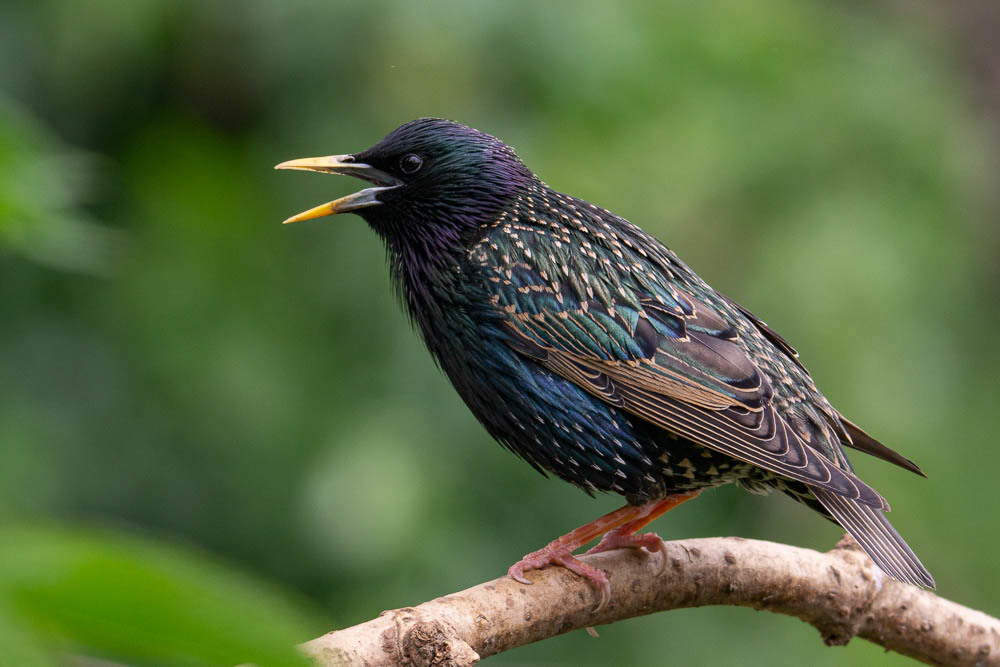
\includegraphics[width=0.6\textwidth]{Problem_5/Figs_P5/fig02.jpg}\caption{Một chú chim sáo đá châu Âu (\textit{Sturnus vulgaris}).}
    \label{fig:Sturn}
\end{figure}

\ \ 

\setcounter{equation}{0}
\begin{center}
    \normalcolor{\textbf{Bài giải}}
\end{center}
\begin{enumerate} 
    \item  \textbf{Enzyme cứng hay mềm ?}\\
    \begin{enumerate}[label=\textbf{\alph*,}]\itemsep0em
        \item Giả sử abzyme biến dạng một lượng $x_1$ và cơ chất biến dạng một lượng $x_2$. Từ trạng thái chuyển tiếp như hình vẽ trong đề bài, cơ chất liên kết với vùng hoạt động, do đó:
        \begin{equation} \label{eq1_enzyme}
            a+x_1=2d-x_2.
        \end{equation}
        Mặt khác, ta có định luật 3 Newton cho cân bằng lực ở vùng hoạt động:
        \begin{equation} \label{eq2_enzyme}
            k_e x_1 = k_s x_2.
        \end{equation}
        Từ phương trình (\ref{eq1_enzyme}) và phương trình (\ref{eq2_enzyme}), ta suy ra $x_1$ và $x_2$:
        \begin{equation} \label{eq3_enzyme}
        \begin{split}
            x_1=\dfrac{k_s}{k_e+k_s}(2d-a),\\
            x_2=\dfrac{k_e}{k_e+k_s}(2d-a).
        \end{split}
        \end{equation}
        Năng lượng cung cấp cho enzyme gây ra biến dạng của enzyme là:
        \begin{equation} \label{eq4_enzyme}
            E_e=\dfrac{1}{2}k_e x_1^2 =  \dfrac{k_e k_s^2}{2(k_e+k_s)^2}(2d-a)^2. 
        \end{equation}
        Năng lượng cung cấp cho cơ chất gây ra biến dạng của cơ chất là:
        \begin{equation} \label{eq5_enzyme}
            E_s=\dfrac{1}{2}k_s x_2^2 =  \dfrac{k_s k_e^2}{2(k_e+k_s)^2}(2d-a)^2. 
        \end{equation}
    \item Lấy phương trình (\ref{eq4_enzyme}) chia cho phương trình (\ref{eq5_enzyme}), ta thu được liên hệ về năng lượng:
    \begin{equation} \label{eq6_enzyme}
        \dfrac{E_e}{E_s}=\dfrac{k_s}{k_e}.
    \end{equation}
    Như ta đã biết, một enzyme xúc tác càng hiệu quả sẽ tiêu tốn càng ít năng lượng cho việc biến dạng chính nó, hay chính là $E_e \ll E_s$, tương đương với $k_e \gg k_s$. Do đó, một enzyme hoạt động hiệu quả sẽ phải thật "cứng" để phần lớn năng lượng được sử dụng vào biến dạng của cơ chất, từ đó thúc đẩy phản ứng hoá học.\\
    \textit{Trong mô hình này, ta xét abzyme do abzyme chỉ dùng tương tác van der Waals, các enzyme tự nhiên sử dụng cả liên kết cộng hoá trị nên "cứng" hơn nhiều abzyme, do đó mà khả năng xúc tác phản ứng cũng mạnh hơn nhiều lần.}
    \end{enumerate}
    \item \textbf{Bỏ qua động năng?}\\
    \begin{enumerate}[label=\textbf{\alph*,}]\itemsep0em
        \item Phương trình động lực học:
        \begin{equation} \label{eq7_enzyme}
        \begin{split}
            m\dfrac{d^2 x}{dt^2}&=F_{\text{ela}}\\
            \rho V \dfrac{d^2 x}{dt^2}&= - \dfrac{ES}{D}x \\
            \dfrac{d^2 x}{dt^2}+&\dfrac{E}{\rho D^2}x=0.    
        \end{split}
        \end{equation}
        Đặt $\dfrac{E}{\rho D^2}=\omega_0^2$, phương trình (\ref{eq7_enzyme}) trở thành:
        \begin{equation} \label{eq8_enzyme}
            \dfrac{d^2 x}{dt^2}+\omega_0^2 x=0.
        \end{equation}
        Chu kỳ dao động của enzyme:
        \begin{equation} \label{eq9_enzyme}
            T_0=\dfrac{2\pi}{\omega_0}=2\pi \sqrt{\dfrac{\rho D^2}{E}}=2.51 \times 10^{-11} \ \si{s}.
        \end{equation}
        \item 
        \begin{enumerate}
            \item Ta có phương trình động lực học như sau:
        \begin{equation} \label{eq10_enzyme}
        \begin{split}
            m\dfrac{d^2 x}{dt^2} &=F_{\text{vis}}+F_{\text{ela}}\\
            \rho V \dfrac{d^2 x}{dt^2} &=-10 \eta D \dfrac{dx}{dt} - \dfrac{ES}{D}x \\
            \dfrac{d^2 x}{dt^2}+ &\dfrac{10\eta }{\rho D^2}\dfrac{dx}{dt}+\dfrac{E}{\rho D^2}x=0.
        \end{split}
        \end{equation}
        Đặt $\dfrac{10\eta }{\rho D^2}=2\beta$, phương trình (\ref{eq10_enzyme}) trở thành:
        \begin{equation} \label{eq11_enzyme}
            \dfrac{d^2 x}{dt^2}+2\beta\dfrac{dx}{dt}+\omega_0^2 x=0.
        \end{equation}
        Trong đó:
        \begin{equation} \label{eq12_enzyme}
            \beta = \dfrac{5\eta}{\rho D^2}=3.125\times 10^{11} \ \si{s^{-1}}, \quad \omega_0=\sqrt{\dfrac{E}{\rho D^2}}=2.5\times 10^{11}\ \si{s^{-1}}.
        \end{equation}
        Phương trình vi phân (\ref{eq10_enzyme}) có nghiệm là:
        \begin{equation} \label{eq13_enzyme}
            x(t)=Ae^{\lambda_1t}+Be^{\lambda_2t}.
        \end{equation}
        Trong đó:
        \begin{align} \label{eq14_enzyme}
            \lambda_1&=-\beta+\sqrt{\beta^2-\omega_0^2}=-1.25\times 10^{11} \ \si{s^{-1}},\\
            \label{eq15_enzyme}
            \lambda_2&=-\beta-\sqrt{\beta^2-\omega_0^2}=-5\times 10^{11} \ \si{s^{-1}}.
        \end{align}
        Tại $t=0$, $x(0)=x_0$ và $v(0)=x'(0)=0$, suy ra $A=\dfrac{\lambda_2 x_0}{\lambda_2-\lambda_1}=\dfrac{4}{3} x_0$ và $B=\dfrac{\lambda_1 x_0}{\lambda_1-\lambda_2}=-\dfrac{1}{3} x_0$.\\
        Nghiệm của phương trình vi phân (\ref{eq10_enzyme}) có thể viết lại thành:
        \begin{equation} \label{eq16_enzyme}
            x(t)=x_0\left(\dfrac{4}{3}e^{\lambda_1t}-\dfrac{1}{3}e^{\lambda_2t}\right).
        \end{equation}
        Trong đó $\lambda_1=-1.25\times 10^{11} \ \si{s^{-1}}$ và $\lambda_2=-5\times 10^{11} \ \si{s^{-1}}$.
    \begin{figure}[htp]
    \centering
    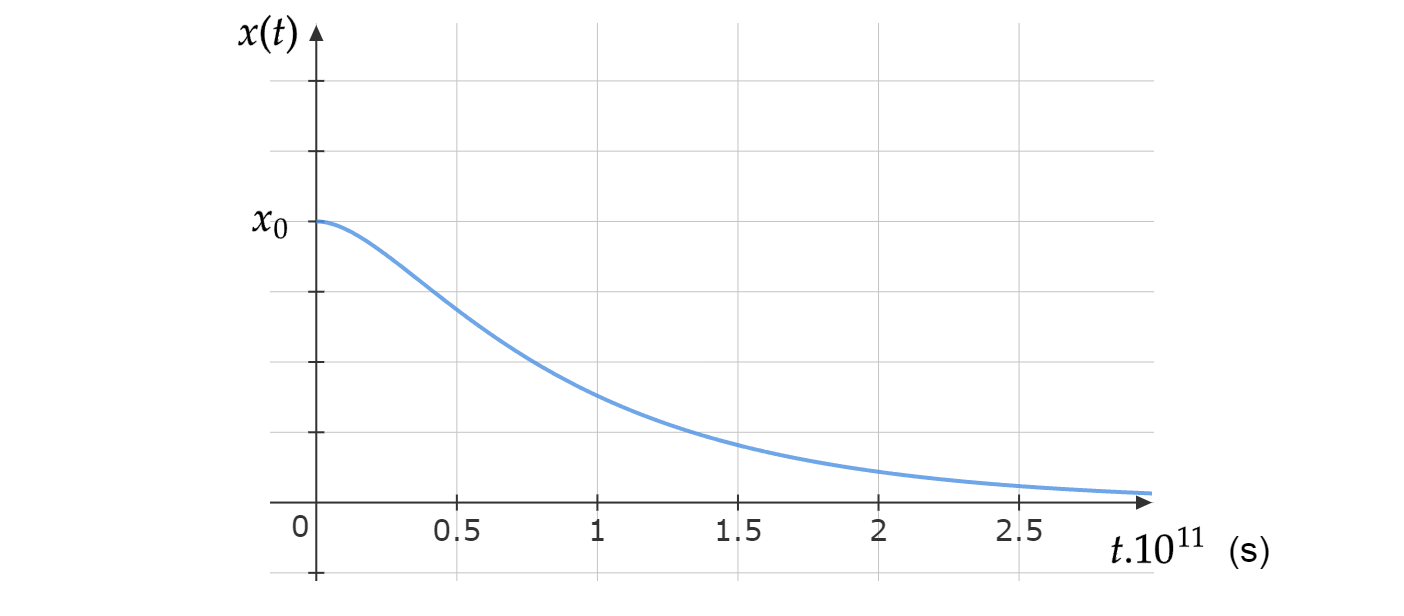
\includegraphics[scale=.27
        ]{Problem_5/image/3.png}
    \caption{Đồ thị $x(t)$.}
    \end{figure}
        \item Tại $t=T_0$, tỉ lệ giữa li độ $x$ và li độ $x_0$ ở thời điểm ban đầu:
        \begin{equation} \label{eq17_enzyme}
            N_1=\dfrac{x(T_0)}{x_0}=\dfrac{4}{3}e^{\lambda_1T_0}-\dfrac{1}{3}e^{\lambda_2T_0} \approx 5.78 \times 10^{-2}.
        \end{equation}
        Tại $t=2T_0$, tỉ lệ giữa li độ $x$ và li độ $x_0$ ở thời điểm ban đầu:
        \begin{equation} \label{eq18_enzyme}
            N_2=\dfrac{x(2T_0)}{x_0}=\dfrac{4}{3}e^{2\lambda_1T_0}-\dfrac{1}{3}e^{2\lambda_2T_0} \approx 2.51 \times 10^{-3}.
        \end{equation}
        
        \textit{Nhận xét: Ta thấy rằng động năng của enzyme bị phân tán và chuyển hoá thành nhiệt quá nhanh (thực tế là trước khi nó có thể được sử dụng trong quá trình xúc tác của enzyme). Quá trình dao động của enzyme hầu như không xảy ra hoặc bị tắt rất nhanh khi chúng ở trong nước (chưa kể đến môi trường nhớt hơn như màng). Do đó trong quá trình xúc tác của enzyme, ta bỏ qua động năng và coi enzyme tĩnh hoặc gần tĩnh.
        \newpage
        Qua bài tập này ta kết luận được hai tính chất rất đặc biệt của enzyme:
        \begin{enumerate}
            \item Năng lượng được cung cấp không phải để thay đổi cấu trúc enzyme mà phần lớn để đưa cơ chất vào enzyme và đưa nó vào trạng thái chuyển tiếp. Do đó vùng hoạt động của enzyme phải là cấu trúc cứng.
            \item Động năng không dùng trong quá trình xúc tác vì nó tiêu tán ra môi trường quá nhanh. Do đó có thể coi các mô hình là tĩnh hoặc gần tĩnh.
        \end{enumerate}}
        \end{enumerate}
    \end{enumerate}
\end{enumerate}

\textbf{Biểu điểm}
\begin{center}
\begin{tabular}{|>{\centering\arraybackslash}m{1cm}|>{\raggedright\arraybackslash}m{14cm}| >{\centering\arraybackslash}m{1cm}|}
    \hline
    \textbf{Phần} & \textbf{Nội dung} & \textbf{Điểm} \\
    \hline
    \textbf{1a} & Viết biểu thức cho $x_1$ và $x_2$ theo $k_e$, $k_s$, $d$ và $a$ (\ref{eq3_enzyme}) & $0.50$ \\
    \cline{2-3}
    &  Viết biểu thức cho $E_e$ theo $k_e$, $k_s$, $d$ và $a$ (\ref{eq4_enzyme}) & $0.25$ \\
    \cline{2-3}
    &  Viết biểu thức cho $E_s$ theo $k_e$, $k_s$, $d$ và $a$ (\ref{eq5_enzyme}) & $0.25$ \\
    \hline
    \textbf{1b} & Lập luận và kết luận & $0.25$ \\
    \hline
    \textbf{2a} & Dẫn ra phương trình vi phân (\ref{eq8_enzyme}) & $0.25$ \\
    \cline{2-3}
    & Tính được chu kỳ dao động $T$ (\ref{eq9_enzyme}) & $0.25$ \\
    \hline
    \textbf{2b.i} & Dẫn ra phương trình vi phân (\ref{eq10_enzyme}) & $0.25$ \\
    \cline{2-3}
    & Viết biểu thức $x(t)$ và các hệ số (\ref{eq16_enzyme}) & $1.25$ \\
    \hline
    \textbf{2b.ii} & Tính được tỉ lệ giữa li độ $x$ và $x_0$ tại thời điểm $t=T_0$ (\ref{eq17_enzyme}) & $0.25$ \\
    \cline{2-3}
    & Tính được tỉ lệ giữa li độ $x$ và $x_0$ tại thời điểm $t=2T_0$ (\ref{eq18_enzyme}) & $0.25$ \\
    \cline{2-3}
    & Lập luận và kết luận & $0.25$ \\
    \hline
\end{tabular}
\end{center}

%% Reference %%
\bibliographystyle{plain}
\begin{thebibliography}{}
\bibitem{bandaria2008} Jigar N. Bandaria, Samrat Dutta, Sarah E. Hill, Amnon Kohen, Christopher M. Cheatum (2008), \textit{Fast Enzyme Dynamics at the Active Site of Formate Dehydrogenase}, Journal of the American Chemical Society, 130(1), 22–23.           
\bibitem{giaotrinh} Nguyễn Thế Toàn, Nguyễn Hoạ Mi (2021), \textit{Giáo trình Vật lý Sinh học của Protein}, NXB ĐHQGHN.
\end{thebibliography}

\newpage
{\normalcolor \textbf{CÂU 6 (4 điểm)}}\vspace{1.5mm}

\setcounter{equation}{0}
Một chiếc khung có bao gồm 5 thanh cứng đồng chất khối lượng $m$ vài có chiều dài $l$ được nối với sàn và nối với nhau bằng các chốt tạo thành lục giác với các cạnh bằng nhau và nằm đối xứng 2 bên (như hình vẽ). Xem rằng không có các ma sát tại các chốt nối. Gọi góc $\alpha$ là góc tạo bởi một thanh ở bên với mặt phẳng nằm ngang. Gia tốc trọng trường là $g$.

\vspace{-3mm}
\begin{center}
\begin{minipage}{0.4\textwidth}
\hspace{0.15\textwidth}
    \begin{tikzpicture}
        %Sàn
        \draw (-2.5,0)--(2.5,0);
        \multiput(-2.5,0)(0.1,0){51}{\line(1,-3){0.12}}
        %Thanh
        \draw[very thick] (-1,0)--(-2,1.7)--(-1,3.4)--(1,3.4)--(2,1.7)--(1,0);
        %Khớp nối
        \filldraw[color=black, fill=ColorOr, ultra thick](-1,0) circle (0.1);
        \filldraw[color=black, fill=ColorOr, ultra thick](1,0) circle (0.1);
        \filldraw[color=black, fill=ColorOr, ultra thick](-2,1.7) circle (0.1);
        \filldraw[color=black, fill=ColorOr, ultra thick](2,1.7) circle (0.1);
        \filldraw[color=black, fill=ColorOr, ultra thick](-1,3.4) circle (0.1);
        \filldraw[color=black, fill=ColorOr, ultra thick](1,3.4) circle (0.1);
        %Ký hiệu
        \draw[->] (2.2,3.3)--(2.2,2.3);
        \draw (2.3,2.8) node[right]{$\vec{g}$};
        \draw (-1.2,0.3) arc (120:180:0.3);
        \draw (-1.8,0.2) node[right]{$\alpha$};
        \draw[thick,->] (0,3.4)--(0,4.4);
        \draw (0.1,3.9) node[right]{$\vec{F}$};
        \filldraw[color=white, fill=white, ultra thick](0,4.3) circle (0.1);
        \draw[<->] (-2.3,0)--(-2.3,3.4);
        \draw (-2.3,1.7) node[left]{$x$};
        \draw[thick,->] (0,3.4)--(0,4.4);
        \draw (0.1,3.9) node[right]{$\vec{F}$};
    \end{tikzpicture}
\end{minipage}    
\hspace{0.1\textwidth}
\begin{minipage}{0.4\textwidth}
    \begin{tikzpicture}
        %Sàn
        \draw (-2.5,0)--(2.5,0);
        \multiput(-2.5,0)(0.1,0){51}{\line(1,-3){0.12}}
        %Thanh
        \draw[very thick] (-1,0)--(-2,1.7)--(-1,3.4)--(1,3.4)--(2,1.7)--(1,0);
        %Khớp nối
        \filldraw[color=black, fill=ColorOr, ultra thick](-1,0) circle (0.1);
        \filldraw[color=black, fill=ColorOr, ultra thick](1,0) circle (0.1);
        \filldraw[color=black, fill=ColorOr, ultra thick](-2,1.7) circle (0.1);
        \filldraw[color=black, fill=ColorOr, ultra thick](2,1.7) circle (0.1);
        \filldraw[color=black, fill=ColorOr, ultra thick](-1,3.4) circle (0.1);
        \filldraw[color=black, fill=ColorOr, ultra thick](1,3.4) circle (0.1);
        %Ký hiệu
        \draw (-1.2,0.3) arc (120:180:0.3);
        \draw (-2.0,0.2) node[right]{$\alpha$};
        \filldraw[color=black, fill=gray, ultra thick](0,4.3) circle (0.1);
        \draw[thick,->] (0,4.3)--(0,3.5);
        \draw (0.1,4) node[right]{$\vec{v}_0$};
    \end{tikzpicture}
\end{minipage}    
\end{center}

\noindent \textbf{1.} Ta đặt vào tâm của thanh ở giữa một lực $F$ theo phương thẳng đừng hướng từ dưới lên trên. Xác định gia tốc góc các thanh $\ddot{\alpha}$ ở bên tại thời điểm cơ hệ đang đứng yên tạm thời ($\dot{\alpha}=0$) theo $m$, $g$, $F$ và $\alpha$. 

\noindent \textbf{2.} Xét trường hợp lực $F$ đặt vào giữa thanh ở giữa theo phương từ dưới lên trên và độ lớn có dạng $F=k(x_0-x)$ với $x$ là khoảng cách từ sàn tới độ cao của thanh ở giữa, $k$ và $x_0$ là các hằng số. Tại vị trí góc $\alpha=\alpha_0$, hệ khung đạt trạng thái cân bằng bền.
\begin{enumerate}[label=\textbf{\alph*,}]\itemsep0em
    \item Tìm hằng số $x_0$ theo $l$, $m$, $g$, $k$ và $\alpha_0$.
    \item Tính chu kỳ dao động nhỏ của hệ quanh vị trí cân bằng bền theo $l$, $m$, $g$, $k$ và $\alpha_0$.
\end{enumerate}
\noindent \textbf{3.} Bỏ qua lực $F$ đặt vào hệ ở các phần trước. Tại thời điểm $\alpha=\alpha_1$ và $\dot{\alpha}=0$, một vật nhỏ có khối lượng $M$ có vận tốc $v_0$ theo phương thẳng đứng chiều từ trên xuống dưới đập vào tâm thanh ở giữa. Xem rằng va chạm này là va chạm hoàn toàn đàn hồi và thời gian va chạm vô cùng ngắn sao cho tọa độ của các vật thay đổi không đáng kể trong quá trình va chạm.
\begin{enumerate}[label=\textbf{\alph*,}]\itemsep0em
    \item Tính vận tốc góc $\dot{\alpha}$ của các thanh ở hai bên ngay sau va chạm.
    \item Tính vận tốc $v$ của vật nhỏ ngay sau va chạm.
\end{enumerate}

\begin{flushright}
    (Biên soạn bởi Log)
\end{flushright}
\setcounter{equation}{0}
\begin{center}
    \normalcolor{\textbf{Bài giải}}
\end{center}
\noindent \textbf{Lời giải chính thức:}

\noindent \textbf{1.}
Động năng của hệ khung là:
\begin{equation} \label{eq1_P1_d2}
    K = m l^2 \dot{\alpha}^2 \left( \dfrac{2}{3} + 4 \cos^2 \alpha \right).
\end{equation}
Thế năng trọng trường của hệ so với mặt đất:3
\begin{equation} \label{eq2_P1_d2}
    U = 6 mgl \sin \alpha.
\end{equation}
Công của lực $F$ và thế năng được chuyển hóa thành động năng của hệ khung, theo định lý động năng dạng vi phân:
\begin{equation} \label{eq3_P1_d2}
    dK = -dU + Fdx \Rightarrow \dfrac{dK}{d \alpha} = - \dfrac{dU}{d \alpha} + F \dfrac{dx}{d \alpha}.
\end{equation}
Thế (\ref{eq1_P1_d2}) và (\ref{eq2_P1_d2}) vào (\ref{eq3_P1_d2}), sử dụng phép đạo hàm $ \dfrac{d (\dot{\alpha}^2)}{d \alpha} =\dfrac{1}{\dot{\alpha}} \dfrac{d (\dot{\alpha}^2)}{dt} = 2 \ddot{\alpha} $ và $\dfrac{dx}{d \alpha}= 2 l \cos \alpha$, ta được
\begin{equation} \label{eq4_P1_d2}
    2 ml^2 \left( \dfrac{2}{3} + 4 \cos^2 \alpha \right) \ddot{\alpha} - 8 m l^2 \dot{\alpha}^2 \cos \alpha \sin \alpha  = -6mgl \cos \alpha + 2 F l \cos \alpha.
\end{equation}
Tại thời điểm $\dot{\alpha}=0$, ta tìm được gia tốc góc của các thanh ở bên là:
\begin{equation} \label{eq5_P1_d2}
    \ddot{\alpha} = \dfrac{(F-3mg) \cos \alpha}{2 ml \left( \dfrac{1}{3} + 2 \cos^2 \alpha \right) }.
\end{equation}
\noindent \textbf{2.} \\
\noindent \textbf{a,} Áp dụng kết quả phần \textbf{1}, để hệ cân bằng thì tại thời điểm thả bất kì không vận tốc đầu thì ta đều có $\ddot{\alpha}=0$, tức là
\begin{equation} \label{eq6_P1_d2}
    F=3mg.
\end{equation}
Tại vị trí cân bằng, lực $F=k(x_0 - 2l \sin \alpha_0)$ nên 
\begin{equation} \label{eq7_P1_d2}
    x_0 = 2l \sin \alpha_0 + \dfrac{3mg}{k}.
\end{equation} 
\noindent \textbf{b,} Để khảo sát dao động nhỏ, ta đặt $\alpha= \alpha_0 + \delta \alpha$ với $\delta \alpha \ll \alpha_0$. Như vậy, ta có thể viết biểu thức lực $F$ theo độ lệch nhỏ $\delta \alpha$ như sau:
\begin{equation} \label{eq8_P1_d2}
    F = k [ x_0 - \sin (\alpha_0 + 2l \delta \alpha)] \approx 3mg - 2kl \cos \alpha_0 \delta \alpha.
\end{equation}
Trong dao động nhỏ, ta có thể bỏ qua các số hạng bậc 2 trong biểu thức lực gia tốc như $\dot{\alpha}^2$, tức là ta có thể sử dụng trực tiếp biểu thứ (\ref{eq5_P1_d2}) để xác định gia tốc góc:
\begin{equation} \label{eq9_P1_d2}
    \delta \ddot{\alpha} = \ddot{\alpha} \approx - \dfrac{k \cos^2 \alpha_0}{m \left( \dfrac{1}{3} + 2 \cos^2 \alpha_0 \right) } \delta \alpha.
\end{equation}
Từ đó, ta tìm được tần số dao động là
\begin{equation} \label{eq10_P1_d2}
    \omega = \sqrt{ \dfrac{k \cos^2 \alpha_0}{m \left( \dfrac{1}{3} + 2 \cos^2 \alpha_0 \right) } }.
\end{equation}
Tức là hệ dao động nhỏ với chu kỳ
\begin{equation} \label{eq11_P1_d2}
    T = 2 \pi \sqrt{ \dfrac{m \left( \dfrac{1}{3} + 2 \cos^2 \alpha_0 \right)}{k \cos^2 \alpha_0} }.
\end{equation}
\noindent \textbf{3.} Gọi $v$ là vận tốc của vật nhỏ sau va chạm. \\
Do va chạm hoàn toàn đàn hồi và động năng của hệ được bảo toàn:
\begin{equation} \label{eq12_P1_d2}
    \dfrac{1}{2} M v_0^2 = \dfrac{1}{2} M v^2 + m l^2 \dot{\alpha}^2 \left( \dfrac{2}{3} + 4 \cos^2 \alpha \right).
\end{equation}
Ta mô hình xung lực mà vật nhỏ tác dụng lên bộ khung bằng một lực $F$ có hướng ngược lại với hướng lực $F$ ở phần \textbf{1} tác dụng trong khoảng thời gian rất ngắn $\Delta t$. Như vậy, theo định lý biến thiên động lượng với vật nhỏ, ta có
\begin{equation} \label{eq13_P1_d2}
    F \Delta t = M (v+v_0).
\end{equation}
Xem rằng ảnh hưởng của $\dot{\alpha}^2$ trong biểu thức lực trong quá trình va chạm rất nhanh là nhỏ và bỏ qua được, ta áp dụng biểu thức (\ref{eq5_P1_d2}) nhưng với chiều của lực $F$ là ngược lại, thành phần liên quan đến trọng lực ở đây có thể xem như rất nhỏ so với xung lực va chạm $F$, như vậy ta tìm được biểu thức thứ hai về liên hệ giữa $v$ và $\dot{\alpha}$ sau va chạm:
\begin{equation} \label{eq14_P1_d2}
    M (v+v_0) = F \Delta t = \dfrac{ ml \left( \dfrac{2}{3} + 4 \cos^2 \alpha \right) }{ \cos \alpha} \ddot{\alpha} \Delta t =  \dfrac{ ml \left( \dfrac{2}{3} + 4 \cos^2 \alpha \right) }{ \cos \alpha} \dot{\alpha}.
\end{equation}
Để thuận tiện, ta sẽ viết lại các phương trình (\ref{eq12_P1_d2}) và (\ref{eq14_P1_d2}) theo một cách gọn gàng hơn một chút:
\begin{itemize}
    \item Từ phương trình (\ref{eq14_P1_d2}), ta được:
    \begin{equation} \label{eq15_P1_d2}
        v+v_0 = \dfrac{ ml \left( \dfrac{2}{3} + 4 \cos^2 \alpha \right) }{ M \cos \alpha} \dot{\alpha}.
    \end{equation}
    \item Hệ phương trình ta có được là một hệ phương trình bậc 1 giả bậc 2, như mọi bài toán va chạm đàn hồi khác, ta sẽ viết lại phương trình (\ref{eq12_P1_d2}) như sau:
    \begin{equation} \label{eq16_P1_d2}
        (v_0-v)(v_0+v) = 2 \dfrac{ml^2 \dot{\alpha}^2}{M} \left( \dfrac{2}{3} + 4 \cos^2 \alpha \right).
    \end{equation}
    Chia (\ref{eq16_P1_d2}) cho (\ref{eq15_P1_d2}), ta được:
    \begin{equation} \label{eq17_P1_d2}
        v_0-v = 2l \dot{\alpha} \cos \alpha.
    \end{equation}
\end{itemize}
Hệ phương trình (\ref{eq15_P1_d2}) và (\ref{eq17_P1_d2}) là hệ phương trình bậc nhất 2 ẩn, từ đó, ta dễ dàng giải được:

\noindent \textbf{a,} Vận tốc góc các thanh ở bên sau va chạm:
\begin{equation} \label{eq18_P1_d2}
    \dot{\alpha} = \dfrac{v_0}{l} \left[ \dfrac{m}{M \cos \alpha} \left( \dfrac{1}{3} + 2 \cos^2 \alpha \right) + \cos \alpha \right]^{-1}.
\end{equation}
\noindent \textbf{b,} Vận tốc của vật nhỏ sau va chạm:
\begin{equation} \label{eq19_P1_d2}
    v = v_0 \dfrac{ \dfrac{m}{M \cos \alpha} \left( \dfrac{1}{3} + 2 \cos^2 \alpha \right) - \cos \alpha }{ \dfrac{m}{M \cos \alpha} \left( \dfrac{1}{3} + 2 \cos^2 \alpha \right) + \cos \alpha }.
\end{equation}

\vspace{6mm}

\noindent \textbf{Lời giải bằng động phương pháp tách vật và lực gia tốc (với sự giúp đỡ của bạn Đinh Đức Thiện):}

\noindent \textbf{1.}

\begin{center}
\begin{minipage}{0.4\textwidth}
\hspace{0.15\textwidth}
    \begin{tikzpicture}
        %Sàn
        \draw (-2.5,0)--(2.5,0);
        \multiput(-2.5,0)(0.1,0){51}{\line(1,-3){0.12}}
        %Thanh
        \draw[very thick] (-1,0)--(-2,1.7)--(-1,3.4)--(1,3.4)--(2,1.7)--(1,0);
        %Khớp nối
        \filldraw[color=black, fill=ColorOr, ultra thick](-1,0) circle (0.1);
        \filldraw[color=black, fill=ColorOr, ultra thick](1,0) circle (0.1);
        \filldraw[color=black, fill=ColorOr, ultra thick](-2,1.7) circle (0.1);
        \filldraw[color=black, fill=ColorOr, ultra thick](2,1.7) circle (0.1);
        \filldraw[color=black, fill=ColorOr, ultra thick](-1,3.4) circle (0.1);
        \filldraw[color=black, fill=ColorOr, ultra thick](1,3.4) circle (0.1);
        %Ký hiệu
        \draw[->] (2.2,3.3)--(2.2,2.3);
        \draw (2.3,2.8) node[right]{$\vec{g}$};
        \draw (-1.2,0.3) arc (120:180:0.3);
        \draw (-1.8,0.2) node[right]{$\alpha$};
        \draw[thick,->] (0,3.4)--(0,4.4);
        \draw (0.1,3.9) node[right]{$\vec{F}$};
        \filldraw[color=white, fill=white, ultra thick](0,4.3) circle (0.1);
        % \draw[<->] (-2.3,0)--(-2.3,3.4);
        % \draw (-2.3,1.7) node[left]{$x$};
        \draw[thick,->] (0,3.4)--(0,4.4);
        \draw (0.1,3.9) node[right]{$\vec{F}$};
        \draw[thick,->] (-1,3.4)--(-1,4.4);
        \draw (-1,3.9) node[right]{$\vec{N}_{1y}$};
        \draw[thick,->] (-1,3.4)--(-2,3.4);
        \draw (-1.7,3.4) node[below]{$\vec{N}_{1x}$};
        \draw[thick,->] (-2,1.7)--(-2,2.5);
        \draw (-1.8,2.1) node[right]{$\vec{N}_{2y}$};
        \draw[thick,->] (-2,1.7)--(-2.8,1.7);
        \draw (-2.4,1.7) node[below]{$\vec{N}_{2x}$};
    \end{tikzpicture}
\end{minipage}
\end{center}
\vspace{3mm}

Gọi $N_{1x}$ và $N_{1y}$ là hình chiếu của lực một thanh ở bên tác dụng lên thanh trên cùng. $N_{2x}$ và $N_{2y}$ là hình chiếu của lực một thanh bên phía dưới tác dụng lên thanh bên phía trên (như hình vẽ).

Định luật 2 Newton cho thanh trên cùng
\begin{equation} \label{eq20_P1_d2}
    F - mg + 2N_{1y} = m \dfrac{d^2}{dt^2} \left( 2 l \sin \alpha \right) = 2ml \left( - \dot{\alpha}^2 \sin \alpha + \ddot{\alpha} \cos \alpha \right).
\end{equation}
Định luật 2 Newton cho chuyển động khối tâm thanh bên phía trên theo 2 phương
\begin{equation} \label{eq21_P1_d2}
    -mg - N_{1y} + N_{2y} = m \dfrac{d^2}{dt^2} \left( \dfrac{3}{2} l \sin \alpha \right) = \dfrac{3}{2} ml \left( - \dot{\alpha}^2 \sin \alpha + \ddot{\alpha} \cos \alpha \right).
\end{equation}
Và
\begin{equation} \label{eq22_P1_d2}
    - N_{1x} + N_{2x} = m \dfrac{d^2}{dt^2} \left( \dfrac{1}{2} l \cos \alpha \right) = \dfrac{1}{2} ml \left( - \dot{\alpha}^2 \cos \alpha - \ddot{\alpha} \sin \alpha \right).
\end{equation}
Định luật 2 Newton chuyển động quay cho tâm quay khối tâm thanh bên phía trên
\begin{equation*}
    -\left( N_{1x} + N_{2x} \right) \dfrac{1}{2} l \cos \alpha - \left( N_{1y} + N_{2y} \right) \dfrac{1}{2} l \sin \alpha = \dfrac{1}{12} m l^2 \ddot{\alpha}.
\end{equation*}
Hay
\begin{equation} \label{eq23_P1_d2}
    -\left( N_{1x} + N_{2x} \right)\cos \alpha - \left( N_{1y} + N_{2y} \right) \sin \alpha = \dfrac{1}{6} m l \ddot{\alpha}.
\end{equation}
Định luật 2 Newton tâm quay cố định của thanh bên phía dưới
\begin{equation*}
    -mg \dfrac{1}{2} l \cos \alpha + N_{2x} l \cos \alpha - N_{2y} l \sin \alpha = \dfrac{1}{3} m l^2 \ddot{\alpha}.
\end{equation*}
Hay
\begin{equation} \label{eq24_P1_d2}
    -mg \cos \alpha + 2 N_{2x} \cos \alpha - 2 N_{2y} \sin \alpha = \dfrac{2}{3} m l \ddot{\alpha}.
\end{equation}
Giải hệ phương trình (\ref{eq20_P1_d2}), (\ref{eq21_P1_d2}), (\ref{eq22_P1_d2}), (\ref{eq23_P1_d2}) và (\ref{eq24_P1_d2}), với $\dot{\alpha}=0$, ta xác định được gia tốc góc các thanh ở bên là
\begin{equation*}
    \ddot{\alpha} = \dfrac{(F-3mg) \cos \alpha}{2 ml \left( \dfrac{1}{3} + 2 \cos^2 \alpha \right) }.
\end{equation*}

\noindent \textbf{2.} Giống như lời giải chính thức.

\noindent \textbf{3.} Coi xung lực trao đổi giữa thanh và vật nhỏ là $F$ như phần \textbf{1.} nhưng ngược hướng. Giống như lời giải chính thức, ta thu được phương trình (\ref{eq13_P1_d2}).

Hệ 5 phương trình  (\ref{eq20_P1_d2}), (\ref{eq21_P1_d2}), (\ref{eq22_P1_d2}), (\ref{eq23_P1_d2}) và (\ref{eq24_P1_d2}) trong phần này sẽ trở thành:
\begin{equation} \label{eq25_P1_d2}
    F \Delta t + 2N_{1y} \Delta t = 2ml \dot{\alpha} \cos \alpha.
\end{equation}
\begin{equation} \label{eq26_P1_d2}
    - N_{1y} \Delta t + N_{2y} \Delta t = \dfrac{3}{2} ml  \dot{\alpha} \cos \alpha.
\end{equation}
\begin{equation} \label{eq27_P1_d2}
    - N_{1x} \Delta t + N_{2x} \Delta t = - \dfrac{1}{2} ml \dot{\alpha} \sin \alpha.
\end{equation}
\begin{equation} \label{eq28_P1_d2}
    -\left( N_{1x} \Delta t + N_{2x} \Delta t \right)\cos \alpha - \left( N_{1y} \Delta t + N_{2y} \Delta t \right) \sin \alpha = \dfrac{1}{6} m l \dot{\alpha}.
\end{equation}
\begin{equation} \label{eq29_P1_d2}
    2 N_{2x} \Delta t \cos \alpha - 2 N_{2y} \Delta t \sin \alpha = \dfrac{2}{3} m l \dot{\alpha}.
\end{equation}
Giải hệ phương trình (\ref{eq25_P1_d2}), (\ref{eq26_P1_d2}), (\ref{eq27_P1_d2}), (\ref{eq28_P1_d2}) và (\ref{eq29_P1_d2}), ta thu được phương trình (\ref{eq14_P1_d2}). Phần còn lại của lời giải sẽ trở về như lời giải chính thức.

\vspace{5mm}

\textbf{Biểu điểm}
\begin{center}
\begin{tabular}{|>{\centering\arraybackslash}m{1cm}|>{\raggedright\arraybackslash}m{14cm}| >{\centering\arraybackslash}m{1cm}|}
    \hline
\textbf{Phần} & \textbf{Nội dung} & \textbf{Điểm} \\
    \hline
    \textbf{1} & Viết động năng $K$ (\ref{eq1_P1_d2}) & $0.25$ \\
    \cline{2-3}
    & Viết thế năng $U$ (\ref{eq2_P1_d2}) & $0.25$ \\
    \cline{2-3}
    & Áp dụng định lý biến thiên động năng (\ref{eq4_P1_d2}) & $0.25$ \\
    \cline{2-3} 
    & Tính được gia tốc góc $\ddot{\alpha}$ & $0.25$ \\
    \hline
    \textbf{2a} & Xác định điều kiện để cân bằng (\ref{eq6_P1_d2}) & $0.25$ \\
    \cline{2-3}
    & Tính $x_0$ (\ref{eq7_P1_d2}) & $0.25$ \\
    \hline
    \textbf{2b} & Viết phương trình dao động điều hòa (\ref{eq9_P1_d2}) & $0.25$ \\
    \cline{2-3}
    & Tìm được chu kỳ dao động (\ref{eq11_P1_d2}) & $0.25$ \\
    \hline
    \textbf{3a} & Viết phương trình bảo toàn năng lượng (\ref{eq12_P1_d2}) & $0.25$ \\
    \cline{2-3}
    & Viết được liên hệ thứ hai giữa $v$ và $\dot{\alpha}$ (\ref{eq14_P1_d2}) & $0.75$ \\ 
    \hline
    \textbf{3b} & Tính vận tốc góc $\dot{\alpha}$ (\ref{eq18_P1_d2}) & $0.50$ \\
    \cline{2-3} 
    & Tính vận tốc vật sau va chạm $v$ (\ref{eq19_P1_d2}) & $0.50$ \\
    \hline
\end{tabular}
\end{center}

\noindent \textbf{Mở rộng vấn đề:}

\indent Đây là một bài toán có liên kết tương đối phức tạp, dù hệ khung chỉ có 1 bậc tự do nhưng việc sử dụng lực và gia tốc để giải quyết bài toán này như lời giải thứ hai được đưa ra trở nên rất phức tạp trong tính toán, đòi hỏi người giải phải vận dụng khéo léo các kiến thức ta có.

\indent Ở phần \textbf{1}, sử dụng định lý động năng có thể xem là cách làm hiệu quả nhất. Việc định nghĩa ra một hàm thế năng cho lực $F$ và đưa bài toán về bảo toàn năng lượng là một cách làm không chặt chẽ vì lực $F$ không thể chắc rằng nó là một lực thế, song, cách làm này có thể chấp nhận được vì lực là một đại lượng không phụ thuộc vào lịch sử, quá trình, với bất kỳ một quá trình khác nhau nào nhưng có cùng một giá trị của lực ứng với một trạng thái xác định, các thông tin về cơ hệ tại thời điểm đó cũng là tương đương và kết quá vẫn là chính xác.

\indent Phần \textbf{3} của bài toán là một phần có thể nói là rất khó về ý tưởng vật lý đối với học sinh THPT. Thường ở các bài toán va chạm, ta sẽ sử dụng các phương trình bảo toàn để lập hệ phương trình và giải. Tuy nhiên trong bài toán này, ta không thể thấy một động lượng hay một momen động lượng ứng với một trục nào được bảo toàn. Cách dẫn dắt và lời giải của bài toán cũng đã đưa ra một cách giải quyết tạm thời ổn thỏa.\\% Cho một lời giải thích tổng quát và mạnh hơn, bạn có thể tìm đọc về định lý Noether trong cơ học Lagrange.\\
% Cho một ý tưởng dị hợm hơn để giải quyết bài toán này, ta có thể nhận ra hệ khung này có cơ cấu tương tự với một hệ khung gồm 3 thanh cứng tạo thành hình thoi, 2 thanh ở 2 bên nặng $2m$, dài $2l$ và thanh ở giữa nặng $m$, dài $l$ như hình vẽ dưới đây:

% \begin{center}
% \begin{minipage}{0.4\textwidth}
% \hspace{0.15\textwidth}
%     \begin{tikzpicture}
%         %Sàn
%         \draw (-2.5,0)--(2.5,0);
%         \multiput(-2.5,0)(0.1,0){51}{\line(1,-3){0.12}}
%         %Thanh
%         \draw[very thick] (-1,0)--(-3,3.4)--(-1,3.4)--(1,0);
%         %Khớp nối
%         \filldraw[color=black, fill=ColorOr, ultra thick](-1,0) circle (0.1);
%         \filldraw[color=black, fill=ColorOr, ultra thick](1,0) circle (0.1);
%         \filldraw[color=black, fill=ColorOr, ultra thick](-3,3.4) circle (0.1);
%         \filldraw[color=black, fill=ColorOr, ultra thick](-1,3.4) circle (0.1);
%         %Ký hiệu
%         \draw (-1.2,0.3) arc (120:180:0.3);
%         \draw (-1.8,0.2) node[right]{$\alpha$};
%     \end{tikzpicture}
% \end{minipage}    
% \end{center}

% Hệ khung này đã được đưa vào bài 1 đề thi TST 2005 ngày 1 và có thể sử dụng bảo toàn momen động lượng để giải quyết bài toán.\\
Bài toán này được lấy ý tưởng từ các bài: Bài cơ học TST 2016,  Bài 1 ngày 1 TST 2005, Bài 1 ngày 1 TST 2001, Bài 48 trong quyển sách "200 more puzzling Physics problems" của  Péter Gnädig , Gyula Honyek và Mate Vigh, bài 1.30 trong quyển sách "A guide to physics problems" tập 1 của Sidney B. Cahn và Boris E. Nadgorny. 

\newpage
{\normalcolor \textbf{CÂU 7 (4 điểm)}}\vspace{1.5mm}

\setcounter{equation}{0}
Có một sợi dây hình trụ bằng vật liệu đồng chất dẫn điện dẫn nhiệt, biết rằng khi nhiệt độ môi trường là $ T_{0} $ thì chiều dài của nó là $ l_{0} $, bán kính là $ r_{0} $ và điện trở suất của nó là $ \rho_{0} $.
Điện trở suất của vật liệu thay đổi theo nhiệt độ theo hàm $ \rho (T) = \rho_{0} \left (1+ \beta \left (T-T_{0} \right) \right) $, hệ số giãn nở tuyến tính là $\alpha$. Bây giờ một dòng điện có cường độ $ I $ chạy vào và đợi cho hệ cân bằng nhiệt. Biết rằng theo vật liệu toả nhiệt ra môi trường với hệ số $\lambda$ với công suất
$$\left(\frac{dQ}{dt}\right)_{\text{loss}} = \lambda S (T - T_0),$$




\begin{minipage}{0.76\textwidth}
với $S$ là diện tích bề mặt toả nhiệt.

\begin{enumerate}[label=\textbf{\alph*,}]\itemsep0em
\item Giả sử rằng hình trụ dẫn nhiệt tốt và nhiệt độ tại mỗi vị trí là như nhau khi nó ổn định, hãy tính nhiệt độ $ T_{f} $ lúc cân bằng (khai triển đến bậc nhất của $\alpha$, $\beta$).
\item Giả sử rằng hình trụ dài và nhiệt độ khác nhau tại các vị trí khác nhau trong quá trình cân bằng, điện trở suất và sự nở vì nhiệt được bỏ qua (nghĩa là lấy $ \alpha = \beta = 0 $), hệ số dẫn nhiệt Fourier $ k $ là một hằng số và nhiệt độ ở cả hai đầu được giả định là $ T_{0} $, hãy tìm phân bố nhiệt độ $ T (x) $ trên khối trụ. 
\end{enumerate}
\end{minipage}
\begin{minipage}{0.35\textwidth}
\quad \quad
  \begin{tikzpicture}[scale=0.85]
\draw[dashed](0,1.5,0)--(0,-1.5,0);
\draw[thick,-stealth](0,-3)--(0,-1.5);
    \draw[dashed] (1.5,0) arc (0:180:1.5cm and 0.6cm);
    \draw[dashed] (1.5,-1.5) arc (0:180:1.5cm and 0.5cm);
	\shade[shading=radial, inner color=orange!20!white, outer color=orange!60!white, opacity=0.70] (1.5,1.5) -- (1.5,-1.5) arc (360:180:1.5cm and 0.5cm) -- (-1.5,1.5) arc (180:360:1.5cm and 0.5cm) ;
	\draw[] (1.5,1.5) -- (1.5,-1.5) arc (360:180:1.5cm and 0.5cm) -- (-1.5,1.5) arc (180:360:1.5cm and 0.5cm) ;
  \draw[dashed] (1.5,0) arc (360:180:1.5cm and 0.6cm);
  \shade[shading=radial, inner color=orange!20!white, outer color=orange!60!white, opacity=0.70] (1.5,1.5) arc (0:360:1.5cm and 0.5cm); 
  \draw (1.5,1.5) arc (0:360:1.5cm and 0.5cm);
  \draw [dashed] (0,1.5)--(1.5,1.5);
	\node at (0.8,1.7) {$r_0$};
\draw[thick,-stealth](0,1.5)--(0,3);
\draw (0,-2.5) node[right]{$I$};
\draw (0,2.5) node[right]{$I$};
\end{tikzpicture}	
\end{minipage}

\vspace{1.5mm}
\textit{Gợi ý: Nghiệm tổng quát của phương trình vi phân tuyến tính thuần nhất $ y ^{\prime \prime} -A y + B = 0$ $(A> 0) $ là} 
$$ y = \cfrac{B}{A} + C_{1} e ^{ \sqrt{A} x} + C_{2} e ^{- \sqrt{A} x} ,$$
\textit{với $C_1$ và $C_2$ là các hằng số được xác định từ các điều kiện ban đầu.}

\begin{flushright}
    (Biên soạn bởi Zinc và Yukon)
\end{flushright}
\setcounter{equation}{0}
\begin{center}
    \normalcolor{\textbf{Bài giải}}
\end{center}
\begin{enumerate}[label = \textbf{\arabic*.}]\itemsep0em 
        \item Công suất bức xạ trên một đơn vị diện tích tại khoảng cách \(d_{S-E}\) là: \\
        \begin{equation} \label{eq1_greenhouse_effect}
            F = \frac{L}{4\pi d_{S-E}^2}.
        \end{equation}
        Ta nhận thấy diện tích thu bức xạ hiệu dụng của Trái Đất là \(\pi R_e^2\) và diện tích phát xạ là \(4 \pi R_e^2\) (\(R_e\) là bán kính Trái Đất). Áp dụng định luật Stefan-Boltzmann cho vật đen tuyệt đối và cân bằng nhiệt, ta thu được:
        \begin{equation} \label{eq2_greenhouse_effect}
            F \pi R_e^2 = \sigma 4 \pi R_e^2 T_0^4 \Rightarrow T_0 = \sqrt[4]{\dfrac{F}{4 \sigma}} = \sqrt[4]{\frac{L}{16 \pi \sigma d_{S-E}^2}} = 278.36 \ \si{K}.
        \end{equation}
        \item Công suất bức xạ từ Mặt Trời tới Trái Đất trung bình trên một đơn vị diện tích bề mặt Trái Đất là:
        \begin{equation} \label{eq3_greenhouse_effect}
            F_{avg} = F\frac{\pi R_e^2}{4 \pi R_e^2} = \frac{F}{4} = \frac{L}{16 \pi d_{S-E}^2}.
        \end{equation}
        % Ta có sơ đồ như sau, tham khảo từ \textbf{Fig. 7-12} sách \textit{Introduction to Atmospheric Chemistry}, D. Jacob: 
\tikzset{every picture/.style={line width=0.75pt}} %set default line width to 0.75pt        
\begin{center}
\begin{tikzpicture}[x=0.75pt,y=0.75pt,yscale=-1,xscale=1]
%uncomment if require: \path (0,300); %set diagram left start at 0, and has height of 300

%Straight Lines [id:da017040213830761708] 
\draw    (50,251) -- (520,251) ;
%Straight Lines [id:da39350620490124144] 
\draw    (50,111) -- (521,111) ;
%Straight Lines [id:da5746750899334658] 
\draw    (285.5,111) -- (285.02,54.67) ;
\draw [shift={(285,52.67)}, rotate = 89.51] [color={rgb, 255:red, 0; green, 0; blue, 0 }  ][line width=0.75]    (10.93,-3.29) .. controls (6.95,-1.4) and (3.31,-0.3) .. (0,0) .. controls (3.31,0.3) and (6.95,1.4) .. (10.93,3.29)   ;
%Straight Lines [id:da42230087156008556] 
\draw    (285.5,111) -- (285.98,157.67) ;
\draw [shift={(286,159.67)}, rotate = 269.41] [color={rgb, 255:red, 0; green, 0; blue, 0 }  ][line width=0.75]    (10.93,-3.29) .. controls (6.95,-1.4) and (3.31,-0.3) .. (0,0) .. controls (3.31,0.3) and (6.95,1.4) .. (10.93,3.29)   ;
%Straight Lines [id:da9183624557930194] 
\draw    (169,21.33) -- (169.99,256.33) ;
\draw [shift={(170,258.33)}, rotate = 269.76] [color={rgb, 255:red, 0; green, 0; blue, 0 }  ][line width=0.75]    (10.93,-3.29) .. controls (6.95,-1.4) and (3.31,-0.3) .. (0,0) .. controls (3.31,0.3) and (6.95,1.4) .. (10.93,3.29)   ;
%Straight Lines [id:da5136183708350828] 
\draw    (180,251.33) -- (179.01,19.33) ;
\draw [shift={(179,17.33)}, rotate = 89.76] [color={rgb, 255:red, 0; green, 0; blue, 0 }  ][line width=0.75]    (10.93,-3.29) .. controls (6.95,-1.4) and (3.31,-0.3) .. (0,0) .. controls (3.31,0.3) and (6.95,1.4) .. (10.93,3.29)   ;
%Straight Lines [id:da012398922733801054] 
\draw    (451,251.33) -- (451,188.33) ;
\draw [shift={(451,186.33)}, rotate = 90] [color={rgb, 255:red, 0; green, 0; blue, 0 }  ][line width=0.75]    (10.93,-3.29) .. controls (6.95,-1.4) and (3.31,-0.3) .. (0,0) .. controls (3.31,0.3) and (6.95,1.4) .. (10.93,3.29)   ;
%Straight Lines [id:da8922550794799347] 
\draw    (450,100.33) -- (450,48.33) ;
\draw [shift={(450,46.33)}, rotate = 90] [color={rgb, 255:red, 0; green, 0; blue, 0 }  ][line width=0.75]    (10.93,-3.29) .. controls (6.95,-1.4) and (3.31,-0.3) .. (0,0) .. controls (3.31,0.3) and (6.95,1.4) .. (10.93,3.29)   ;

% Text Node
\draw (539.14,240.85) node [anchor=north west][inner sep=0.75pt]  [rotate=-0.9] [align=left] {$\displaystyle T_{s}$};
% Text Node
\draw (529,100) node [anchor=north west][inner sep=0.75pt]   [align=left] {$\displaystyle T_{a}$};
% Text Node
\draw (299,74) node [anchor=north west][inner sep=0.75pt]   [align=left] {$\displaystyle \varepsilon _{a} \sigma T_{a}^{4}$};
% Text Node
\draw (298,120) node [anchor=north west][inner sep=0.75pt]   [align=left] {$\displaystyle \varepsilon _{a} \sigma T_{a}^{4}$};
% Text Node
\draw (122,137) node [anchor=north west][inner sep=0.75pt]   [align=left] {$\displaystyle F_{avg}$};
% Text Node
\draw (183,138.83) node [anchor=north west][inner sep=0.75pt]   [align=left] {$\displaystyle \alpha F_{avg}$};
% Text Node
\draw (463,218) node [anchor=north west][inner sep=0.75pt]   [align=left] {$\displaystyle \sigma T_{s}^{4}$};
% Text Node
\draw (456,64) node [anchor=north west][inner sep=0.75pt]   [align=left] {$\displaystyle ( 1-\varepsilon _{a}) \sigma T_{s}^{4}$};
\end{tikzpicture} \\
\vspace{3mm}
Hình 1: Sơ đồ nhận nhiệt và bức xạ của trái đất và khí quyển. \cite{Jacob}
\end{center}
        Xét cân bằng nhiệt của lớp khí quyển, ta thu được phương trình đầu tiên:
        \begin{equation} \label{eq4_greenhouse_effect}
            2\varepsilon_a \sigma T_a^4 = \varepsilon_a \sigma T_s^4.
        \end{equation}
        Xét cân bằng nhiệt của cả hệ mặt đất và khí quyển, ta thu được phương trình thứ hai:
        \begin{equation} \label{eq5_greenhouse_effect}
            F_{avg}(1-\alpha) = (1-\varepsilon_a)\sigma T_s^4 + \varepsilon_a \sigma T_a^4.
        \end{equation}
        Giải phương trình (\ref{eq4_greenhouse_effect}) và (\ref{eq5_greenhouse_effect}), ta thu được:
        \begin{align} \label{eq6_greenhouse_effect}
            T_s &= \sqrt[4]{\frac{L(1-\alpha)}{8\pi \sigma d^2_{S-E}(2-\varepsilon_a)}} = 290 \ \si{K},\\
        \label{eq7_greenhouse_effect}
            T_a &= \sqrt[4]{\frac{L(1-\alpha)}{16\pi \sigma d^2_{S-E}(2-\varepsilon_a)}} = 243 \ \si{K}.
        \end{align}
        \item Thay (\ref{eq4_greenhouse_effect}) xuống (\ref{eq5_greenhouse_effect}), ta được:
        \begin{equation} \label{eq8_greenhouse_effect}
            \frac{2 F_{avg}(1-\alpha)}{\sigma} = (2 - \varepsilon_a) T_s^4.
        \end{equation}
        Vì vế trái không đổi khi \(T_s ,\ \varepsilon_a\) thay đổi, lấy ln rồi vi phân hai vế để vế trái bằng $0$, ta thu được:
        \begin{equation} \label{eq9_greenhouse_effect}
            -\frac{\Delta \varepsilon_a}{2-\varepsilon_a} + \frac{4 \Delta T_s}{T_s} = 0 \Rightarrow \Delta T_s = \frac{T_s}{4(2-\varepsilon_a)} \Delta \varepsilon_a,
        \end{equation}
        cho nên
        \begin{equation} \label{eq10_greenhouse_effect}
        k = \frac{T_s}{4(2-\varepsilon_a)}. % \approx 61.2.
        \end{equation}
    \end{enumerate}
\textit{Nhận xét: Một điều thú vị có thể rút ra từ ý \textbf{2} là bề mặt Trái Đất hấp thụ lượng bức xạ từ khí quyển gần như tương đương so với bức xạ từ Mặt Trời!}
\vspace{5mm}

\textbf{Biểu điểm}
\begin{center}
\begin{tabular}{|>{\centering\arraybackslash}m{1cm}|>{\raggedright\arraybackslash}m{14cm}| >{\centering\arraybackslash}m{1cm}|}
    \hline
    \textbf{1} & Tính công suất bức xạ trên một đơn vị $F$ (\ref{eq1_greenhouse_effect}) & $0.50$ \\
    \cline{2-3}
    & Áp dụng định luật Stefan-Boltzmann và tính nhiệt độ trái đất $T_0$ (\ref{eq2_greenhouse_effect}) & $0.50$ \\
    \hline
    \textbf{2} & Viết phương trình cân bằng nhiệt đối với khí quyển (\ref{eq4_greenhouse_effect}) & $0.75$ \\
    \cline{2-3}
    & Viết phương trình cân bằng nhiệt đối với hệ trái đất và khí quyển (\ref{eq5_greenhouse_effect}) & $0.75$ \\
    \cline{2-3}
    & Giải hệ phương trình và tính nhiệt độ trái đất và khí quyển (\ref{eq6_greenhouse_effect}) \& (\ref{eq7_greenhouse_effect}) & $0.50$ \\
    \hline
    \textbf{3} & Viết biểu thức liên hệ giữa $\varepsilon_a$ và $T_S$ (\ref{eq8_greenhouse_effect}) & $0.50$ \\
    \cline{2-3}
    & Tính $k$ (\ref{eq10_greenhouse_effect}) & $0.50$ \\
    \hline
\end{tabular}
\end{center}

%% Reference %%
\bibliographystyle{plain}
\begin{thebibliography}{}
\bibitem{Jacob} Jacob, D (1999). \textit{Introduction to Atmospheric Chemistry}. Princeton University Press.
\bibitem{Randall} Randall, D.A. (2012). \textit{Atmosphere, Clouds and Climate}. Princeton University Press.
\end{thebibliography}

\newpage
{\normalcolor \textbf{CÂU 8 (4 điểm)}}\vspace{1.5mm}

\setcounter{equation}{0}
Máy co góc plasma (\textit{Angular pinch}) sử dụng từ trường để tăng tốc và định hướng dòng plasma, do đó nó có thể tạo ra một vụ nổ plasma tại một mục tiêu ngay lập tức. Thiết bị được thể hiện trên hình dưới. Có một tấm dẫn xung quanh ống thủy tinh chân không và chứa một thanh mục tiêu có cùng chiều dài, bỏ qua độ dày của thành ống thủy tinh và độ dày của vỏ ruột dẫn, và $ H \gg R_{ 2} $. Ống chứa đầy hiđro bị ion hóa thành plasma có mật độ số điện tích dương và âm đều là $n$. Khi $ t = 0 $, người ta đặt một nguồn điện vào vỏ dây dẫn để dòng điện tăng nhanh từ 0 đến $ I $ và dòng điện $ I $ được giữ nguyên trong một khoảng thời gian, dòng điện chạy đều dọc theo hướng tiếp tuyến của vỏ hình trụ. Bỏ qua chuyển động nhiệt của các hạt, tương tác Coulomb và va chạm giữa các hạt, điện tích nguyên tố là $ e $, khối lượng của các electron và hạt nhân hydro lần lượt là $ m_{e}, m_{p} $.

\begin{figure}[!htb]
    \centering
    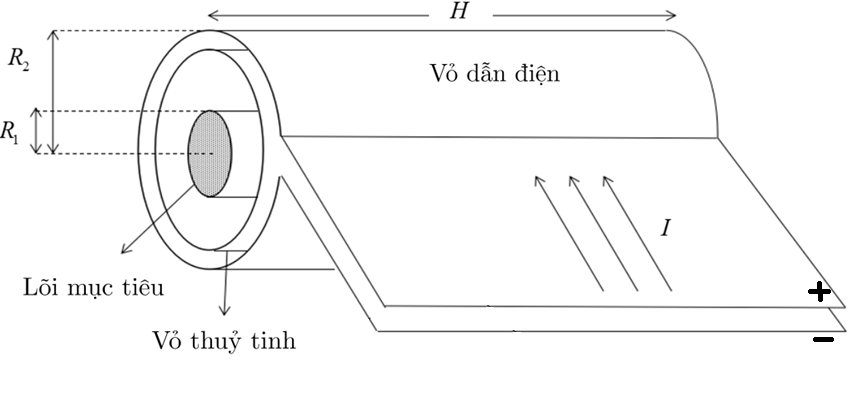
\includegraphics[scale=0.55]{Problem_8/P8.png}
    \label{fig_P8}
\end{figure}
\begin{enumerate}[label=\textbf{\alph*,}]\itemsep0em
\item Một hạt có điện tích $ q $ và khối lượng $ m $ ở khoảng cách từ trục trung tâm $ r \left (R_{1} <r <R_{2} \right) $ sau khi dòng điện ổn định tới $ I $. Tìm tốc độ tức thời $ v_{0} $ của hạt.    
    \item Tìm thời điểm $ t (r) $ khi hạt trong câu hỏi trước chuyển động đến vị trí $ R_{1} $.
    \item Giả sử hạt va chạm với thanh mục tiêu hoàn toàn không đàn hồi, tìm áp suất $ P (t) $ trên bề mặt của thanh mục tiêu tại thời điểm $ t $. Trên thực tế, plasma trong ống là các electron và hạt nhân hydro bị ion hóa, điều này cho thấy chuyển động của một loại hạt có thể bị bỏ qua khi $ t $ nhỏ, và ảnh hưởng của hạt này cần được bỏ qua trong câu trả lời cuối cùng.
    \item Xác định thông số thiết bị $ \beta = \cfrac {P_{\max}} {\omega_{B}} $, trong đó $ \omega_{B} $ là mật độ năng lượng của từ trường chân không và độ lớn của nó là $ \cfrac {B^{2}} {2 \mu_{0}} $. Sau đó, so sánh nó với $ \beta \left(\approx 10^{-1} \sim 1 \right) $ của hầu hết các thiết bị Tokamak (định hướng dòng plasma dạng donut) và thể hiện những ưu điểm của máy co góc. Đối với phép tính số trong câu hỏi này, hãy thay $\cfrac{\mu_{0}}{4 \pi} = 1 \times 10^{- 7} \mathrm {~N} / \mathrm {A}^{2}$, $H = 30.0 \mathrm {~m}$, $R_{1} = 1.0 \mathrm{~mm}$, $R_{2} = 1.00 \mathrm{~m}$, $n = 1.00 \times 10^{8} \mathrm {~m}^{-3}$.
\end{enumerate}

\begin{flushright}
    (Biên soạn bởi Zinc và Yukon)
\end{flushright}
\setcounter{equation}{0}
\begin{center}
    \normalcolor{\textbf{Bài giải}}
\end{center}
\textbf{a,} Chọn hệ tọa độ trụ ($r$, $\phi$, $z$) sao cho chiều tăng của $\phi$ trùng với chiều dòng điện qua trụ.

Ta có từ trường bên trong trụ là đều và bằng:
\begin{equation} \label{eq1_p3_d2}
\vec{B} = \mu_0 \frac{i}{H} \hat{z},
\end{equation}
với $i$ là dòng điện tức thời trên trụ.

Do đối xứng, khi từ trường tăng lên khi dòng điện tăng, sẽ có điện trường xoáy theo phương $\hat{\boldsymbol{\phi}}$. 
Điện trường này sẽ gây một xung lượng lên các hạt điện tích trong khoảng không bên trong trụ.

Theo định luật Faraday
\begin{equation} \label{eq2_p3_d2}
\begin{split}
2\pi r E(r) = \pi r^2 \frac{\partial B}{\partial t}\\
\Rightarrow E = \frac{\mu_0 r}{2 H} \frac{\partial i}{\partial t}.
\end{split}
\end{equation}

Theo định luật Lenz, $E$ hướng ngược chiều $\hat{\boldsymbol{\phi}}$ (là chiều dòng điện gây ra biến thiên từ trường) (giả sử $\displaystyle \frac{\partial i}{\partial t} > 0$).

Có tốc độ mà một hạt tích điện nhận được
\begin{equation} \label{eq3_p3_d2}
\begin{split}
\vec{v}_0 &= \lim_{\Delta t \to 0} \int_0^{\Delta t} \frac{\vec{F}}{m} dt \\
&= - \lim_{\Delta t \to 0} \int_{0}^{I} \frac{\mu_0 qr}{2mH}\hat{\boldsymbol{\phi}} di\\
&= -\frac{\mu_0 qrI}{2mH}\hat{\boldsymbol{\phi}}.
\end{split}
\end{equation}

\textbf{b,} Khi dòng điện đã ổn định, các điện tích chỉ chuyển động trong từ trường.
Do đó tốc độ từng hạt được bảo toàn.

Do từ trường hướng theo trục $\hat{z}$, vận tốc đầu vuông góc với trục $\hat{z}$ nên chuyển động sau đó của hạt nằm trong mặt phẳng vuông góc với $\hat{z}$.

Ký hiệu $R_0$ là tọa độ $r$ ban đầu của hạt ta đang xét.

Như vậy
\begin{equation} \label{eq4_p3_d2}
\begin{split}
\vec{v} &= \dot{r} \hat{r} + r\dot{\phi} \hat{\boldsymbol{\phi}}\\
\Rightarrow |\vec{v}| &= \sqrt{\dot{r}^2 + r^2 \dot{\phi}^2} = v_0.
\end{split}
\end{equation}

Ta nhận thấy trong trường hợp này, momen động lượng của một hạt tích điện (so với trục $z$) không được bảo toàn.
Theo đó
\begin{equation} \label{eq5_p3_d2}
\begin{split}
\frac{d \vec{L}}{d t} &= \vec{r} \times (q \vec{v} \times \vec{B})= q[(\vec{r} \cdot \vec{B})\vec{v} - (\vec{r} \cdot \vec{v})\vec{B}]= -\frac{q\vec{B}}{2} \frac{\partial (r^2)}{\partial t}.
\end{split}
\end{equation}

\begin{equation} \label{eq6_p3_d2}
\begin{split}
\Rightarrow \vec{L} + \frac{qr^2 \vec{B}}{2} &= \mathrm{const}\\
&= -mR_0 v_0 \hat{z} + \frac{qR_0^2 B}{2} \hat{z}\\
&= 0.
\end{split}
\end{equation}
Từ đó tìm được vận tốc $v_{\phi}$ theo phương tiếp tuyến (không xét chiều)
\begin{equation} \label{eq7_p3_d2}
\begin{split}
    v_{\phi} &= \frac{qr^2 B}{2mr}\\
&= \frac{qB}{2m}r.
\end{split}
\end{equation}
Do đó vận tốc theo phương tiếp tuyến $\dot{r}$
\begin{equation} \label{eq8_p3_d2}
\begin{split}
|\dot{r}| &= \sqrt{v_0^2 - \left(\frac{qB}{2m}\right)^2 r^2} \\
&= \frac{qB}{2m} \sqrt{R_0^2 - r^2}.
\end{split}
\end{equation}
Dễ dàng nhận thấy để biểu thức có nghĩa, $r < R_0$ trong suốt quá trình chuyển động. Do đó $\dot{r}$ mang dấu âm.\\
Khoảng thời gian từ khi dòng điện được bật lên cho đến khi vật đang xét đập vào thành trong của ống trụ là
\begin{equation} \label{eq9_p3_d2}
\begin{split}
\tau &= \int_{R_0}^{R_1} -\frac{2m}{qB} \frac{d r}{\sqrt{R_0^2 - r^2}}\\
&= \frac{2m}{qB} \arccos \left(\frac{R_1}{R_0}\right).
\end{split}
\end{equation}

\textbf{c,} Chú ý rằng với $t$ nhỏ, tác động do các hạt có khối lượng bé hơn sẽ là chủ đạo (khối lượng electron nhỏ hơn proton khoảng 2000 lần).\\
Tại thời điểm $t$, các hạt tới từ lớp $r = R(t)$ sẽ đập vào thành trong trụ với $R(t)$ bằng
\begin{equation} \label{eq10_p3_d2}
R(t) = \frac{R_1}{\cos\left(\dfrac{qBt}{2m}\right)}.
\end{equation}
Động lượng mà một hạt truyền cho thành trong trụ khi đập vào là
\begin{equation} \label{eq11_p3_d2}
\begin{split}
p_1 &= m \dot{r}= \frac{qB}{2} \sqrt{R_1^2 \left(\frac{1}{\cos^2 \left(\frac{qBt}{2m}\right)}-1\right)}\\
&= \frac{qBR_1}{2} \tan\left( \dfrac{qBt}{2m}\right).
\end{split}
\end{equation}

Áp suất tác dụng lên thành trong của trụ
\begin{equation} \label{eq12_p3_d2}
\begin{split}
p &= \frac{1}{2\pi R_1 l} \frac{qBR_1}{2} \tan \left(\frac{qBt}{2m}\right) n \cdot 2\pi R(t) \frac{d R}{d t},
\end{split}
\end{equation}
với $R(t)$ là hàm được định nghĩa ở trên.
Đặt $\displaystyle \omega = \frac{qB}{2m}$. 

Ta tìm được áp suất là
\begin{equation} \label{eq13_p3_d2}
p = nm \omega^2 R_1^2 \frac{\sin^2(\omega t)}{\cos^4(\omega t)}.
\end{equation}

\textbf{d,} Ta thấy $p$ là hàm đồng biến theo $t$ (khi $\displaystyle \omega t < \frac{\pi}{2}$).
\begin{equation} \label{eq14_p3_d2}
\begin{split}
p_{max} &= nm \omega ^2 R_2^2 \left[\left(\frac{R_2}{R_1}\right)^2 - 1\right]\\
\Rightarrow \beta &= \frac{p_{max}}{\omega_B} = \frac{\mu_0 n e^2}{2m} R_2^2 \left[\left(\frac{R_2}{R_1}\right)^2 - 1\right].   
\end{split}
\end{equation}
Thế số, ta được $\beta = 1.77 > 1$.

\textbf{Biểu điểm} 
\begin{center}
\begin{tabular}{|>{\centering\arraybackslash}m{1cm}|>{\raggedright\arraybackslash}m{14cm}| >{\centering\arraybackslash}m{1cm}|}
    \hline
    \textbf{Phần} & \textbf{Nội dung} & \textbf{Điểm} \\
    \hline
    \textbf{a} & Tìm được từ trường bên trong trụ (\ref{eq1_p3_d2})  & 0.10\\   
    \cline{2-3}
    &  Tìm được điện trường bên trong trụ theo định luật Faraday (\ref{eq2_p3_d2}) & 0.10 \\
    \cline{2-3}
    & Chú ý rằng vẫn truyền một xung lượng cho hạt tích điện khi $\Delta t \to 0$ & 0.10\\
    \cline{2-3}
    & Tìm được vận tốc truyền cho hạt tích điện (\ref{eq3_p3_d2}) & 0.20\\
    \hline
    \textbf{b} & Nhận ra rằng tốc độ hạt là không đổi và tìm được thành phần vận tốc theo phương bán kính & 0.25\\
    \cline{2-3}
    & Đạo hàm momen động lượng và đưa ra phương trình (\ref{eq6_p3_d2}) (dạng vector hoặc vô hướng) & 0.75\\
    \cline{2-3}
    & Đưa về dạng phương trình vi phân tại (\ref{eq8_p3_d2}) & 0.25 \\
    \cline{2-3}
    & Tích phân để tìm được khoảng thời gian hạt đập vào thành trong (\ref{eq9_p3_d2}) & 0.25 \\
    \hline
    \textbf{c} & Tìm được bán kính đầu của các hạt đập vào thành trong trụ tại thời điểm $t$ (\ref{eq10_p3_d2}) & 0.25\\
    \cline{2-3}
    & Tìm được động lượng mà hạt truyền cho trụ (\ref{eq11_p3_d2}) & 0.50\\
    \cline{2-3}
    & Tìm được dạng cơ bản của áp suất tác dụng lên thành trong trụ (\ref{eq12_p3_d2}) & 0.50 \\
    \cline{2-3}
    & Khai triển và đưa về dạng hoàn chính (\ref{eq13_p3_d2}) & 0.25\\
    \hline
    \textbf{d} & Tìm được $P_{max}$ theo $R_2 / R_1$ (\ref{eq14_p3_d2}) & 0.25\\
    \cline{2-3}
    & Tìm được giá trị (bằng số và biểu thức) của $\beta$ & 0.25\\
    \hline
\end{tabular}
\end{center}

\newpage
{\normalcolor \textbf{CÂU 9 (4 điểm)}}\vspace{1.5mm}

\setcounter{equation}{0}
\textbf{Bức xạ vùng xa}

Trong truyền sóng điện từ không dây, "trường xa" thường được hiểu là trường điện từ ở vị trí xa nguồn phát $r$ hơn nhiều lần bước sóng điện từ $\lambda$. Khi khảo sát ảnh hưởng của trường điện từ tại vùng không gian này, hiện tượng cảm ứng điện từ chiếm ưu thế hoàn toàn so với điện từ trường như trong các mô hình tĩnh điện (định luật Coulomb) hay từ dừng (định luật Bio-Savart-Laplace).

\begin{center}
\begin{minipage}{\textwidth}
\centering
\begin{tikzpicture}[scale=0.8]
    %%Decartes_coordinate
    \draw[-Stealth] (0,0) to (0,5);
    \draw[-Stealth] (0,0) to (5,0);
    \draw[-Stealth] (0,0) to (-4,-3);
    \draw[fill=black] (0,0) circle (0.05);
    \draw 
    (4.5,0) node[above]{$y$}
    (0,4.5) node[left]{$z$}
    (-3.6,-2.6) node[left]{$x$};
    %%Sphere_coordinate
    \draw (0,0) circle (4);
    \draw (0,4) arc(90:-90:2 and 4);
    \draw[dashed] (0,4) arc(90:270:2 and 4);
    \draw (-4,0) arc(180:360:4 and 2);
    \draw[dashed] (4,0) arc(0:180:4 and 2);
    %%projection
    \draw[fill=black] (1.4,2.85) circle (0.05);
    \draw (0,0) to (1.4,2.85) to (1.4,-1.4) to (0,0);
    \draw[dashed] (1.4,-1.4) to (1.75,-1.75);
    \draw[-Stealth] (-0.8,-0.6) arc(-130:-45:1);
    \draw[-Stealth] (0,1) arc(90:63:1);
    \draw 
    (-0.3,-1.2) node{$\phi$}
    (0.25,1.4) node{$\theta$}
    (0.9,1.2) node{$r$};
    %%unit vector
    \draw[-Stealth] (1.4,2.85) to (2,4.1);
    \draw[-Stealth] (1.4,2.85) to (2,1.7);
    \draw[-Stealth] (1.4,2.85) to (2.5,3.3);
    \draw
    (2.2,2.8) node{$\hat{\phi}$}
    (2.1,2.2) node{$\hat{\theta}$}
    (1.5,4) node{$\hat{r}$};
    %%antenna
    \draw[ultra thick, -Stealth] (0,-0.5) to (0,0.5);
    \draw (-0.6,0.1) node{$I,\delta$};
\end{tikzpicture}
\end{minipage} \\
\vspace{2mm} 
Hình 1: Hệ tọa độ cầu và vị trí của dây dẫn.
\end{center}

Theo đó, một đoạn dây dẫn vô cùng ngắn có chiều dài $\delta \ll \lambda$ có dòng điện xoay chiều $I = I_0 \cos \omega t$ chạy qua và tích điện hai đầu dây như một lưỡng cực điện sẽ giống như một nguồn phát sóng điện từ có dạng
\begin{equation*}
    \Vec{E} = - \omega \mu \dfrac{I_0 \delta}{4 \pi r} \sin \left( \omega t - \dfrac{2 \pi r}{\lambda} \right) \sin \theta \hat{\theta}.
\end{equation*}
Và cường độ từ trường
\begin{equation*}
    \Vec{H} = - \omega \sqrt{\mu \varepsilon} \dfrac{I_0 \delta}{4 \pi r} \sin \left( \omega t - \dfrac{2 \pi r}{\lambda} \right) \sin \theta \hat{\phi}.
\end{equation*}

Năng lượng bức xạ của sóng điện từ qua một đơn vị diện tích trong một đơn vị thời gian được biểu diễn qua vector Poynting theo biểu thức
\begin{equation*}
    \Vec{S} = \Vec{E} \times \Vec{H}.
\end{equation*}

\begin{enumerate}
    \item Xét một đoạn dây thẳng có độ dài $l_1 \ll \lambda$ có dòng $I=I_0 \cos \omega t$. 
    \begin{enumerate}
        \item Hãy tìm công suất bức xạ trung bình $P$ của đoạn dây.
        \item Công suất phát xạ sóng điện từ của đoạn dây tiêu hao năng lượng tương đương một thành phần điện trở $R_r$. Hãy xác định điện trở $R_r$.
    \end{enumerate}
    \item Xét một đoạn dây thẳng có độ dài $l_2$ so sánh được với $\lambda$ và có dòng điện $I=I_0 \cos \omega t$ chạy qua. Xét các điểm cùng cách tâm đoạn dây thẳng một khoảng $r$, tìm tỷ số cường độ sóng truyền theo phương hợp với dây một góc $\theta$ và cường độ sóng truyền theo phương $\theta=\pi/2$.
\end{enumerate}

\begin{flushright}
    (Biên soạn bởi Log)
\end{flushright}
\setcounter{equation}{0}
\begin{center}
    \normalcolor{\textbf{Bài giải}}
\end{center}
\textbf{a.} Ta nhận thấy rằng cường độ của các tia ló liên tiếp nhau hơn kém nhau $R^2$ lần, do đó biên độ sóng hơn kém nhau $R$ lần.

Hiệu quang trình của hai tia ló liên tiếp là: $\displaystyle \Delta = 2e \sqrt{n^2 - \sin^2 \theta}$.

Từ đó ta tìm được độ lệch pha của hai tia ló liên tiếp là: $\displaystyle \delta = \frac{2\pi}{\lambda} \delta = \frac{4 \pi e}{\lambda} \sqrt{n^2 - \sin^2 \theta}$.

Dao động tổng hợp của sóng ánh sáng tại vị trí $\theta$ trên màn E là:
\begin{align}
    A(r,t) &= A_0 \cos \left(\omega t - \frac{2\pi}{\lambda} r\right) + A_0 R\cos \left(\omega t - \frac{2\pi}{\lambda} r- \delta\right)\\
    &+ A_0 R^2 \cos \left(\omega t - \frac{2\pi}{\lambda} r- 2\delta\right) + \ldots\\ 
    &= \sum_{n=0}^\infty A_0 R^n \cos \left(\omega t - \frac{2\pi}{\lambda} r- n\delta\right). \label{41}
\end{align}

Tách hàm lượng giác thành hai phần tử thời gian và độ lệch pha, ta có
\begin{align}
    A(r,t) &= A_0 \left[\cos \left(\omega t - \frac{2\pi}{\lambda} r\right) \sum_{n=0}^\infty R^n \cos (n\delta) + \sin \left(\omega t - \frac{2\pi}{\lambda} r\right) \sum_{n=0}^\infty R^n \sin(n\delta) \right]\\
    &= \frac{A_0}{1 + R^2 - 2R \cos \delta} \left[ \cos \left(\omega t - \frac{2\pi}{\lambda} r\right) (1 - R\cos \delta) + R\sin \left(\omega t - \frac{2\pi}{\lambda} r\right) \sin \delta\right]. \label{42}
\end{align}

Cường độ ánh sáng tại vị trí cần tỉ lệ thuận với giá trị trung bình của bình phương biên độ sóng, tức là
\begin{align}
    I(\theta) &\propto \langle A(r,t)^2 \rangle =  \frac{A_0^2}{2} \frac{1}{1 + R^2 - 2R\cos \delta} \label{43}\\
    &\propto \frac{A_0^2}{2} \frac{1}{1 + R^2 -2R \left(1 - 2 \sin^2 \dfrac{\delta}{2} \right)}\\
    &\propto \frac{I(0)}{1 + \dfrac{4R}{(1-R)^2} \sin^2 \dfrac{\delta}{2}}.\label{44}
\end{align}

\textit{*Cách giải khác:} Ta có thể sử dụng phương pháp số phức trong bài toán này, cụ thể là ta đặt biên độ sóng từ tia thứ $n+1$ lúc này là $A = A_0 e^{i(\omega t - k r + n \delta)}$.

Khi đó biên độ tổng hợp của sóng tại vị trí màn là
\begin{align}
    A(r.t) &= A_0 e^{i (\omega t - kr)} \left(1 + R e^{i\delta} + R^2 e^{2i \delta} + R^3 e^{3i \delta} \ldots \right)\\
    &= A_0 e^{i (\omega t - kr)} \frac{1}{1 - R e^{i \delta}}
\end{align}

Cường độ sáng tại vị trí xét sẽ tỉ lệ thuận với tích của $A$ và liên hợp phức của nó $\Bar{A}$:
\begin{align}
    I \propto A \cdot \Bar{A} = \frac{A_0^2}{1 + R^2 - 2 R\cos \delta}.
\end{align}



Từ đó ta tìm được $\displaystyle a = \frac{4R}{(1-R)^2}$ và $\displaystyle \Phi = \delta = \frac{4 \pi e}{\lambda} \sqrt{n^2 - \sin^2 \theta}$.
\vspace{1mm}

\textbf{b.} Để tìm khoảng vân, ta cần tìm các vị trí cực đại liên tiếp, khi $\displaystyle \frac{\delta}{2} = k \pi$ với $k \in \mathbb{Z}$.

Ta có $y = f \sin \theta$ là toạ độ của điểm giao thoa với chùm tia ló góc $\theta$. Khi đó tại vị trí $\theta \approx 0$, ta có
\begin{align}
    k = \frac{2ne}{\lambda}  \sqrt{1 - \frac{\sin^2 \theta}{n^2}} \approx \frac{2ne}{\lambda} \left( 1 - \frac{y^2}{2 n^2 f^2} \right). \label{45}
\end{align}

Tại $y =0$ thì $\displaystyle k_0 =  \frac{2ne}{\lambda}$, tại $y = i$ ($i$ là khoảng vân) thì $k = k_0 -1$. Khi đó ta tìm được khoảng vân là
\begin{align}
    i = f\sqrt{\frac{n\lambda}{e}}.\label{46}
\end{align}


\vspace{1.5mm}

\textbf{c.} Ta tìm được khoảng giá trị của $I(\theta)$ là 
\begin{align}
    I_{\text{max}} &= I_0, \\
    I_{\text{min}} &= \frac{I_0}{1 + a}.
\end{align}

Từ đó ta tìm được độ tương phản giao thoa trên màn
\begin{align}
    \Gamma = \frac{a}{a+2} = \frac{2R}{1+R^2}.
\end{align}

 \textbf{Biểu điểm} 
\begin{center}
\begin{tabular}{|>{\centering\arraybackslash}m{1cm}|>{\raggedright\arraybackslash}m{14cm}| >{\centering\arraybackslash}m{1cm}|}
    \hline
    \textbf{Phần} & \textbf{Nội dung} & \textbf{Điểm} \\
    \hline
    \textbf{a} & Tìm được độ lệch pha $\delta$ & 0.50\\   
    \cline{2-3}
    &  Viết được biên độ tổng hợp trên màn tại $\theta$ (\ref{41}) & 0.50\\
    \cline{2-3}
    & Khai triển tổng chuỗi biên độ (\ref{42}) & 0.50\\
    \cline{2-3}
    & Nhận ra $I \propto \langle A^2 \rangle$ (\ref{43}) & 0.50\\
    \cline{2-3}
    & Viết được hàm $I$ và tìm được $a$ và $\Phi$ (\ref{44}) & 0.50\\
    \hline
    \textbf{b} & Tìm được $k$ (\ref{45}) & 0.50\\
    \cline{2-3}
    & Tìm được khoảng vân $i$ (\ref{46}) & 0.50\\
    \hline
    \textbf{c} & Biểu diễn đúng $\Gamma$ theo $R$ & 0.50 \\
    \hline
\end{tabular}
\end{center}

\newpage
{\normalcolor \textbf{CÂU 10 (4 điểm)}}\vspace{1.5mm}

\setcounter{equation}{0}
\textbf{Tâm sai quỹ đạo trái đất} \\
Quỹ đạo Trái Đất quanh Mặt Trời không phải là một hình tròn hoàn hảo mà là một hình ellipse với tâm sai \(\varepsilon\). Chính vì vậy, thời gian giữa các sự kiện Xuân phân, Hạ chí, Thu phân và Đông chí là không đều nhau. Trong bài tập này, chúng ta sẽ đưa ra một mô hình tính toán tâm sai của trái đất với sai số cỡ $9 \%$ thông qua các thông tin về những ngày đặc biệt trong năm (như bảng dưới). \\
% Một số thông tin cơ bản về hình ellipse: %(em cần ký hiệu bán trục lớn, nhỏ, bán tiêu cự, trục x, y, r và góc của 1 điểm bất kỳ)
% \(a\): Bán trục lớn \\
% \(b\): Bán trục nhỏ \\
% \(c\): Bán tiêu cự \\
% \(\varepsilon\): Tâm sai \\
% Công thức tâm sai:
% \begin{equation*}
%     \varepsilon = \frac{c}{a} = \sqrt{1 - \frac{b^2}{a^2}}
% \end{equation*}
% Phương trình ellipse trong hệ tọa độ Descartes: 
% \begin{equation*}
%     \frac{x^2}{a^2} + \frac{y^2}{b^2} = 1 
% \end{equation*}
% Phương trình ellipse trong hệ tọa độ cực: 
% \begin{equation*}
%     r = \frac{a(1-e^2)}{1 - \varepsilon \cos{\phi}}
% \end{equation*}
\vspace{-0.5cm}
\begin{center}
\footnotesize{
\begin{tabular}{|>{\centering\arraybackslash}m{4cm}|>{\centering\arraybackslash}m{4cm}|>{\centering\arraybackslash}m{3cm}|>{\centering\arraybackslash}m{3cm}|}
    \hline
    Sự kiện & Thời điểm & Thời gian kể từ sự kiện trước (ngày) & Số ngày trôi qua \\
    \hline
    Xuân phân 2022 (VE) & 20/03/2022, 15h33 & - & - \\
    \hline
    Hạ chí 2022 (SS) & 21/06/2022, 09h14 & 92.7368 & 93 \\
    \hline
    Thu phân 2022 (AE) & 23/09/2022, 01h04 & 93.6597 & 93 \\
    \hline
    Đông chí 2022 (WS) & 21/12/2022, 21h48 & 89.8939 & 90 \\
    \hline
    Xuân phân 2023 (VE) & 20/03/2023, 21h24 & 88.9833 & 89 \\
    \hline
\end{tabular} }
\end{center}
\begin{enumerate}[label=\textbf{\arabic*,}]\itemsep0em 
        \item \textbf{Định luật 2 Kepler} \\
        Biểu diễn vận tốc quét \(dS/dt\) theo moment động lượng của Trái Đất \(L_E\) và khối lượng Trái Đất \(m_E\), trong đó \(S\) là diện tích quét được của đường nối Mặt Trời và Trái Đất. Từ đó kiểm nghiệm lại quan sát của Kepler: Diện tích quét được của đường nối hành tinh và Mặt Trời là như nhau trong khoảng thời gian bằng nhau.
        \item \textbf{Xác định tâm sai quỹ đạo Trái Đất}
\vspace{-0.8cm}
\begin{center}
\begin{minipage}{\textwidth}
\centering
\begin{tikzpicture}[scale=0.8]
    \draw[thick] (0,0) ellipse (4 and 2.5);
    \draw[thick, gray] (-8,0) to (8,0);
    \draw[fill=red!60, thick] (-1,0) circle (0.25);
    \draw[dashed, thick, gray] 
    (-4.5,-1.17) to (4.5,1.83)
    (0,-3) to (-2,3);
    \draw[thick, magenta, -Stealth] (-0.4,0) arc (0:290:0.6);
    \draw 
    (-6,0) node[above]{Điểm cận nhật} 
    (6,0) node[below]{Điểm viễn nhật}
    (-1.8,0.7) node{$\phi_{VE}$}
    (-5,-1.4) node{WS}
    (4.8,2) node{SS}
    (-2,3) node[above]{AE}
    (0,-3) node[below]{VE};
\end{tikzpicture}
\end{minipage} \\
\vspace{2mm}
Hình 1: Vị trí bốn sự kiện đặc biệt trong năm.
\end{center}
% \vspace{-0.5cm}
Kí hiệu \(\phi_1\), \(\phi_2\) (\(\phi_2 > \phi_1\)) là góc lượng giác hợp bởi điểm viễn nhật và 2 điểm 1, 2 bất kỳ trên quỹ đạo. Thời gian đi từ 1 đến 2 \(t_{1 \rightarrow 2}\) được cho bởi tích phân sau:
\begin{equation*}
    t_{1 \rightarrow 2} = A \int_{\phi_1}^{\phi_2} \frac{d\phi}{(1-\varepsilon \cos{\phi})^2}.
\end{equation*}
\textbf{a,} Biểu diễn \(A\) theo chu kỳ \(T\) và tâm sai \(\varepsilon\) của trái đất. \\
\textbf{b,} Tâm sai quỹ đạo Trái Đất là nhỏ. Từ phương trình đề bài cho, hãy rút ra xấp xỉ sau:
\begin{equation*}
    t_{1 \rightarrow 2} \approx A[(\phi_2 - \phi_1) + 2\varepsilon(\sin{\phi_2} - \sin{\phi_1})].
\end{equation*}
\textbf{c,} Sử dụng các số liệu cho trong bảng, xử lý và đưa ra tâm sai của quỹ đạo Trái Đất \(\varepsilon\).
\end{enumerate}

\begin{flushright}
    (Biên soạn bởi manhducnmd và Log)
\end{flushright}
\setcounter{equation}{0}
\begin{center}
    \normalcolor{\textbf{Bài giải}}
\end{center}
\begin{enumerate}[label=\textbf{\arabic*,}] 
        \item
        Vi phân diện tích quét của đường nối giữa Trái Đất và Mặt Trời:
        \begin{equation} \label{eq1_Earth_eccentricity}
            dS = \frac{1}{2} r^2 d\phi \Rightarrow\frac{dS}{dt} = \frac{1}{2} r^2 \Dot{\phi}.
        \end{equation}
        Moment động lượng của Trái Đất quanh Mặt trời:
        \begin{equation} \label{eq2_Earth_eccentricity}
            L_E = m_E r v_\phi = m_E r^2 \Dot{\phi} .
        \end{equation}
        Từ đó ta suy ra:
        \begin{equation} \label{eq3_Earth_eccentricity}
            \frac{dS}{dt} = \frac{L_E}{2m_E}.
        \end{equation}
        Do lực hấp dẫn là lực xuyên tâm, momen động lượng của Trái Đất là hằng số, và đại lượng \(dS/dt\) không đổi. Từ đây ta có thể suy ra định luật 2 Kepler.
        \item 
        \begin{enumerate}[label=\textbf{\alph*,}]\itemsep0em
        \item Từ định luật 2 Kepler, ta suy được: 
        \begin{equation} \label{eq4_Earth_eccentricity}
            \frac{S_{1 \rightarrow 2}}{t_{1 \rightarrow 2}} = \frac{\pi ab}{T},
        \end{equation}
        trong đó, $b=a \sqrt{1-\varepsilon^2}$ là bán trục nhỏ của quỹ đạo ellipse. Phần diện tích trái đất quét qua khi đi từ 1 đến 2
        \begin{equation} \label{eq5_Earth_eccentricity}
            S_{1 \rightarrow 2} = \int_{\phi_1}^{\phi_2} \frac{1}{2} r^2 d\phi = \int_{\phi_1}^{\phi_2} \frac{1}{2} \left[ \dfrac{a \left( 1 - \varepsilon^2 \right)^2}{1 - \varepsilon \cos \phi} \right]^2 d \phi.
        \end{equation}
        Thay trở lại biểu thức trên, ta tìm được hằng số $A$ như sau
        \begin{equation} \label{eq6_Earth_eccentricity}
            A = \frac{T (1 - \varepsilon^2)^{\frac{3}{2}}}{2 \pi}.
        \end{equation}
        \item Với $\varepsilon \ll 1$, ta khai triển nhỏ số hạng chứa $\varepsilon$:
        \begin{equation} \label{eq7_Earth_eccentricity}
            \dfrac{1}{\left( 1 - \varepsilon \cos \phi \right)^2} \approx 1 + 2 \varepsilon \cos \phi.
        \end{equation}
        Thay vào biểu thức thời gian di chuyển giữa hai vị trí của trái đất và lấy tích phân, ta thu được
        \begin{equation} \label{eq8_Earth_eccentricity}
            t_{1 \rightarrow 2} \approx A[(\phi_2 - \phi_1) + 2\varepsilon(\sin{\phi_2} - \sin{\phi_1})].
        \end{equation}
        \item Do mỗi sự kiện nối tiếp nhau có góc lệch khi ngắm từ phía trái đất gần đúng là $\pi/2$ nên
        \begin{align}
        & t_{V E \rightarrow S S} \sim A\left[\pi / 2+2 \varepsilon\left(\cos \phi_{V E}-\sin \phi_{V E}\right)\right], \\
        & t_{S S \rightarrow A E} \sim A\left[\pi / 2-2 \varepsilon\left(\sin \phi_{V E}+\cos \phi_{V E}\right)\right], \\
        & t_{A E \rightarrow W S} \sim A\left[\pi / 2-2 \varepsilon\left(\cos \phi_{V E}-\sin \phi_{V E}\right)\right], \\
        & t_{W S \rightarrow V E} \sim A\left[\pi / 2+2 \varepsilon\left(\sin \phi_{V E}+\cos \phi_{V E}\right)\right] .
        \end{align}
        Từ 4 phương trình trên, ta tìm được góc $\phi_{VE}$
        \begin{equation} \label{eq13_Earth_eccentricity}
            \tan \phi_{V E}=\frac{\left(1-\tau_{1}\right)}{\left(1+\tau_{1}\right)},
        \end{equation}
        trong đó
        \begin{equation} \label{eq14_Earth_eccentricity}
            \tau_{1}=\left(\frac{t_{V E \rightarrow S S}-t_{A E \rightarrow W S}}{t_{W S \rightarrow V E}-t_{S S \rightarrow A E}}\right)=\left(\frac{\cos \phi_{V E}-\sin \phi_{V E}}{\cos \phi_{V E}+\sin \phi_{V E}}\right).
        \end{equation}
        Từ bảng số liệu, $\tau_1 \approx -3/4$ và $\varepsilon \approx 4.57 \si{Rad}$.
        Lấy
        \begin{equation} \label{eq15_Earth_eccentricity}
            \tau_{2}=\frac{t_{V E \rightarrow S S}}{t_{A E \rightarrow W S}} = \dfrac{\pi / 2+2 \varepsilon\left(\cos \phi_{V E}-\sin \phi_{V E}\right)}{\pi / 2-2 \varepsilon\left(\cos \phi_{V E}-\sin \phi_{V E}\right)}.
        \end{equation}
        Ta tìm được
        \begin{equation} \label{eq16_Earth_eccentricity}
            \varepsilon \sim \frac{\pi\left(\tau_{2}-1\right)}{4\left(1+\tau_{2}\right)\left(\cos \phi_{V E}-\sin \phi_{V E}\right)} \approx 0.0152.
        \end{equation}
        % (Tham khảo bạn Quân Bảo) 
        Từ 4 phương trình trên, ta thu được hai phương trình: 
        \begin{align}
            & \frac{t_{V E \rightarrow S S}}{t_{A E \rightarrow W S}} = \frac{A\left[\pi / 2+2 \varepsilon\left(\cos \phi_{V E}-\sin \phi_{V E}\right)\right]}{A\left[\pi / 2-2 \varepsilon\left(\cos \phi_{V E}-\sin \phi_{V E}\right)\right]}, \\
            & \frac{t_{W S \rightarrow V E}}{t_{S S \rightarrow A E}} = \frac{A\left[\pi / 2+2 \varepsilon\left(\cos \phi_{V E}+\sin \phi_{V E}\right)\right]}{A\left[\pi / 2-2 \varepsilon\left(\cos \phi_{V E}+\sin \phi_{V E}\right)\right]}. \\
        \end{align}
        Chuyển vế và rút gọn, ta thu được:
        \begin{align}
             & \varepsilon\left(\cos \phi_{V E}-\sin \phi_{V E}\right) =  \frac{\pi \left(t_{V E \rightarrow S S} -t_{A E \rightarrow W S}\right)}{4\left(t_{V E \rightarrow S S} + t_{A E \rightarrow W S}\right)} = a ,\\
             & \varepsilon\left(\cos \phi_{V E}+\sin \phi_{V E}\right) =  \frac{\pi \left(t_{W S \rightarrow V E} -t_{S S \rightarrow A E}\right)}{4\left(t_{W S \rightarrow V E} + t_{S S \rightarrow A E}\right)} = b.
        \end{align}
        Ta rút ra được $\varepsilon \cos \phi_{V E} = (a+b)/2, \varepsilon \sin \phi_{V E} = (a-b)/2$. Cuối cùng,
        \begin{equation} \label{eq22_Earth_eccentricity}
            \varepsilon = \left(\left(\frac{a+b}{2}\right)^2 + \left(\frac{a-b}{2}\right)^2 \right)^{1/2} \approx 0.0166
        \end{equation}
    \end{enumerate}
\end{enumerate}
\textit{Theo số liệu của USNO, tâm sai của trái đất là $\varepsilon = 0.0167$, tức là phép đánh giá thô của chúng ta đã có những hiệu quả nhất định trong việc thiết lập mô hình tính toán tâm sai của trái đất.}

\textit{Lưu ý: Việc khai triển làm xuất hiện các số hạng $\varepsilon$ bậc cao hơn 1 có thể gây ra sai số khá lớn và các đáp án đó sẽ không được chấp nhận.}

\textbf{Biểu điểm}
\begin{center}
\begin{tabular}{|>{\centering\arraybackslash}m{1cm}|>{\raggedright\arraybackslash}m{14cm}| >{\centering\arraybackslash}m{1cm}|}
    \hline
    \textbf{Phần} & \textbf{Nội dung} & \textbf{Điểm} \\
    \hline
    \textbf{1} & Viết biểu thức diện tích quét (\ref{eq1_Earth_eccentricity}) & $0.25$ \\
    \cline{2-3}
    & Viết phương trình bảo toàn momen động lượng (\ref{eq2_Earth_eccentricity}) & $0.50$ \\
    \cline{2-3}
    & Suy ra định luật 2 Kepler (\ref{eq3_Earth_eccentricity}) & $0.25$ \\
    \hline
    \textbf{2a} & Áp dụng định luật 2 Kepler (\ref{eq4_Earth_eccentricity}) & $0.25$ \\
    \cline{2-3}
    & Viết biểu thức diện tích quét & $0.50$ \\
    \cline{2-3}
    & Đối chiếu kết quả và tìm $a$ & $0.25$ \\
    \hline
    \textbf{2b} & Khai triển nhỏ số hạng $\varepsilon$ bậc 1 (\ref{eq7_Earth_eccentricity}) & $0.50$ \\
    \cline{2-3}
    & Lấy tích phân và thu được biểu thức thời gian giữa các sự kiện (\ref{eq8_Earth_eccentricity}) & $0.50$ \\
    \hline
    \textbf{2c} & Từ bảng số liệu xác định $\phi_{VE}$ (\ref{eq13_Earth_eccentricity}) & $0.50$ \\
    \cline{2-3}
    & Tính được giá trị $\varepsilon$ với một phương pháp đúng sai lệch dưới $20\%$ (\ref{eq16_Earth_eccentricity}) & $0.50$ \\
    \hline
\end{tabular}
\end{center}

\bibliographystyle{plain}
\begin{thebibliography}{}
\bibitem{10.1119/5.0127980} B. Cameron Reed. Eccentricity and orientation of Earth’s orbit from equinox and solstice times. \textit{American Journal of Physics}, 91(4):324–326, 04 2023.
\end{thebibliography}

\newpage
{\normalcolor \textbf{CÂU 11 (8 điểm)}}\vspace{1.5mm}

\setcounter{equation}{0}
\textbf{Chảy}

\begin{enumerate}
    \item \textbf{Dòng chảy tầng và định luật Hagen-Poiseuille.} \\
    Định luật Hagen-Poiseuille phát biểu rằng với một dòng chảy không nén và có hệ số nhớt đồng nhất đẳng hướng ở chế độ dừng, thông lượng chất lưu chảy qua một mặt cắt ống sẽ tỷ lệ với chênh lệch áp suất hai đầu ống. \\
    Xét một ống nước thẳng dài có tiết diện ống hình ellipse với độ dài hai bán trục lần lượt là $a$ và $b$. Có một dòng chảy không nén có độ nhớt là $\mu$. Với chênh lệch áp suất hai đầu ống là $\Delta p$ và ống dài $L$, ta có thể đặt $G=\Delta p/L$ là chênh lệch áp suất trên mỗi đơn vị độ dài ống. Ở chế độ chảy dừng ổn định, dòng chảy là dòng chảy tầng, xem rằng các tầng nước có cùng vận tốc nằm theo một đường ellipse trên mặt cắt, hãy tìm phân bố vận tốc theo tọa độ tại các lớp nước và tìm thông lượng nước $Q$ chảy qua một mặt cắt ống trong một đơn vị thời gian theo $G$, $\mu$, $a$ và $b$.
    \item \textbf{Dòng chảy Bernoulli không dừng.} \\
    Một bình nước hình trụ được cấp nước vào sao cho giữ nguyên mực nước cao $h$ so với đáy. Ở gần đáy bình, có một ống nước nằm ngang dài $L$ tiết diện rất nhỏ so với bình xả nước từ bình ra ngoài. Gia tốc trọng trường là $g$. Xem rằng nước trong bình không bị nén. Bỏ qua các ma sát, tổn thất năng lượng ở các đoạn ống, hiệu ứng co hẹp đường ống,... Ban đầu, đầu xả nước bị bịt và toàn bộ nước đứng yên. Tại thời điểm $t=0$, đầu xả nước của ống được mở và nước bắt đầu chảy từ ống ra ngoài. Hãy tìm vận tốc chảy của nước trong ống theo thời gian.
\end{enumerate}

\begin{center}
\begin{minipage}{0.55\textwidth}
    \begin{tikzpicture}[scale=0.8]
        \draw[fill=lightgray, lightgray, ultra thick] (0,0) rectangle (6,4);
        \draw[fill=lightgray, lightgray] (0,2) ellipse (0.5 and 2);
        \draw[ultra thick] (6,0) arc(270:90:0.5cm and 2cm);
        \draw[ultra thick] (6,0) arc(-90:90:0.5cm and 2cm);
        \draw[ultra thick] (0,0) arc(270:90:0.5cm and 2cm);
        \draw[fill=lightgray, ultra thick] (6,2) ellipse (0.5 and 2);
        \draw[ultra thick]
        (0,0) to (6,0)
        (0,4) to (6,4);
        \draw[fill=white, ultra thick] (6,2) ellipse (0.3 and 1.6);
        \draw[dashed] (8,0) rectangle (10,4);
        \draw[dashed] 
        (6,0) to (8,0)
        (6,4) to (8,4);
        \draw[ultra thick] (9,0) arc(270:90:1cm and 2cm);
        \draw[ultra thick] (9,0) arc(-90:90:1cm and 2cm);
        \draw[fill=lightgray, ultra thick] (9,2) ellipse (1 and 2);
        \draw[fill=white, ultra thick] (9,2) ellipse (0.7 and 1.6);
        \draw[Stealth-Stealth] (7.7,0.4) to (7.7,3.6);
        \draw (7.7,2) node[left]{$2a$};
        \draw[Stealth-Stealth] (8.3,-0.3) to (9.7,-0.3);
        \draw (9,-0.3) node[below]{$2b$};
        \draw (5,-1.5) node{Hình 1: Ống trụ có mặt cắt hình ellipse.};
    \end{tikzpicture}
\end{minipage}
\begin{minipage}{0.35\textwidth}
    \begin{tikzpicture}[scale=0.8]
        \draw[fill=blue!30, blue!30] (0,0) to (3,0) to (3,0.1) to (6.5,0.1) to (6.5,0.5) to (3,0.5) to (3,3.6) to (0,3.6) to (0,3.6);
        \draw[ultra thick] (0,4) to (0,0) to (3,0) to (3,0.1) to (6.5,0.1)
        (6.5,0.5) to (3,0.5) to (3,4);
        \draw[dashed] 
        (0,0) to (-0.5,0)
        (0,3.6) to (-0.5,3.6);
        \draw[Stealth-Stealth] (-0.5,0) to (-0.5,3.6);
        \draw (-0.5,1.8) node[left]{$h$};
        \draw[dashed] (6.5,0.5) to (6.5,1);
        \draw[Stealth-Stealth] (3,1) to (6.5,1);
        \draw (4.75,1) node[above]{$L$};

        \draw[-Stealth] (5,3.5) to (5,2.5);
        \draw (5,3) node[right]{$g$};
        \draw (3,-1.5) node{Hình 2: Bình nước hình trụ có ống dài.};
    \end{tikzpicture}
\end{minipage}
\end{center}

\begin{flushright}
    (Biên soạn bởi Log)
\end{flushright}
\setcounter{equation}{0}
\begin{center}
    \normalcolor{\textbf{Bài giải}}
\end{center}
\begin{enumerate}
    \item Với các tầng nước có cùng vận tốc nằm trên một hình ellipse, phân bố vận tốc theo tọa độ có thể viết dưới dạng:
    \begin{equation} \label{eq1_flow}
        u(x,y) = A + B x^2 + C y^2.
    \end{equation}
    Để vận tốc này thỏa mãn điều kiện biên, các phần nước sát thành ống có vận tốc bằng $0$. Tức là, mọi điểm nằm trên đường $1-\dfrac{x^2}{a^2}-\dfrac{y^2}{b^2}=0$, đều có vận tốc bằng $0$. Đối chiếu với phân bố vận tốc trên, ta được
    \begin{equation} \label{eq2_flow}
        u(x,y) = A \left( 1 - \dfrac{x^2}{a^2} - \dfrac{y^2}{b^2} \right).
    \end{equation}
    Định luật 2 Newton với một khối nước có kích thước $\Delta x \times \Delta y \times \Delta z$:
    \begin{equation} \label{eq3_flow}
        \rho \Delta x \Delta y \Delta z \dfrac{\partial u}{\partial t} = ( G \Delta z) \Delta x \Delta y - \dfrac{\partial}{\partial x} \left[ \mu (\Delta y \Delta z)   \dfrac{\partial u}{\partial x} \right] \Delta x - \dfrac{\partial}{\partial y} \left[ \mu  (\Delta x \Delta z) \dfrac{\partial u}{\partial y} \right] \Delta y.
    \end{equation}
    hay ta thu được phương trình Navier-Stokes:
    \begin{equation} \label{eq4_flow}
        \rho \dfrac{\partial u}{\partial t} = G + \mu \dfrac{\partial^2 u}{\partial x^2} + \mu \dfrac{\partial^2 u}{\partial y^2}.
    \end{equation}
    Ở chế độ dừng, $\partial u/ \partial t =0$, nên
    \begin{equation} \label{eq5_flow}
        \dfrac{\partial^2 u}{\partial x^2} + \dfrac{\partial^2 u}{\partial y^2} = - \dfrac{G}{\mu}.
    \end{equation}
    Thay dạng hàm phân bố vận tốc theo tọa độ bên trên vào phương trình này, ta tìm được hệ số $A=\dfrac{G}{2 \mu \left( a^{-2} + b^{-2} \right)}$. Như vậy, ta xác định được phân bố vận tốc các lớp nước theo tọa độ
    \begin{equation} \label{eq6_flow}
        u(x,y) = \dfrac{G}{2 \mu \left( a^{-2} + b^{-2} \right)} \left( 1 - \dfrac{x^2}{a^2} - \dfrac{y^2}{b^2} \right).
    \end{equation}
    Thông lượng dòng qua ống
    \begin{equation} \label{eq7_flow}
        Q = \iint_S u(x,y) dxdy 
    \end{equation}
    Đặt $x=a \rho \cos \theta$ và $y=b \rho \sin \theta$, để lấy tích phân, ta tìm được thông lượng
    \begin{equation} \label{eq8_flow}
        Q = \int_0^1 \dfrac{G a^2 b^2}{2\mu} \left( 1 - \rho^2 \right) 2 \pi ab \rho d \rho 
        = \dfrac{\pi G a^3 b^3}{4 \mu \left( a^2 + b^2 \right)}.
    \end{equation}
    \item Do ta đang khảo sát quá trình không dừng của dòng chảy, vận tốc dòng chảy thay đổi theo thời gian, nên áp dụng trực tiếp phường trình Bernoulli cho dòng chảy dừng là một lời giải sai. Ở đây, ta có 2 cách giải quyết vấn đề này: Cách thứ nhất là ta sẽ áp dụng phương pháp năng lượng và cách thứ hai là tìm lại một phương trình Bernoulli đầy đủ hơn và giải quyết được cả với dòng chảy không dừng. \\
    \textbf{\textit{Cách 1:} Phương pháp năng lượng}\\
    Để mực nước được giữ nguyên, lượng thế năng được cấp vào hệ trong mỗi vi phân thời gian $dt$ là
    \begin{equation} \label{eq9_flow}
        dU = \rho g h S v dt.
    \end{equation}
    Lượng biến đổi động năng hệ trong mỗi vi phân thời gian $dt$ là
    \begin{equation} \label{eq10_flow}
        dK = \rho L S v \dfrac{\partial v}{\partial t} dt + \dfrac{1}{2} \rho S v^3 dt.
    \end{equation}
    Trong đó, số hạng thứ nhất là sự biến đổi động năng gây ra bởi việc dòng nước được tăng tốc khiến động năng của nước trong ống tăng lên và số hạng thứ hai là động năng mà các phần tử nước mang ra ngoài khỏi ống. \\
    Do thể năng nước cấp thêm vào ống gây ra biến đổi về động năng, tức là $dK=dU$, ta thu được biểu thức:
    \begin{equation} \label{eq11_flow}
        L \dfrac{\partial v}{\partial t} + \dfrac{v^2}{2} = \rho g h.
    \end{equation}
    Giải phương trình vi phân trên với điều kiện đầu $t=0$ thì $v=0$, ta được
    \begin{equation} \label{eq12_flow}
        v = \sqrt{2gh} \tanh \left( \dfrac{\sqrt{2gh}}{L} t \right).
    \end{equation}
    \textbf{\textit{Cách 2:} Bổ chính phương trình Bernoulli}\\
    Theo phương trình Navier-Stokes:
    \begin{equation} \label{eq13_flow}
        \rho \dfrac{d \Vec{v}}{dt} = - \nabla p + \rho \Vec{g}.
    \end{equation}
    Đạo hàm toàn phần của $\Vec{v}$ theo thời gian $t$ có thể viết dưới dạng
    \begin{equation} \label{eq14_flow}
        \dfrac{d \Vec{v}}{dt} = \dfrac{\partial \Vec{v}}{\partial t} + \Vec{v} \left( \nabla \cdot \Vec{v} \right).
    \end{equation}
    Nên
    \begin{equation} \label{eq15_flow}
        \dfrac{\partial \Vec{v}}{\partial t} + \Vec{v} \left( \nabla \cdot \Vec{v} \right) + \dfrac{1}{\rho} \nabla p - \Vec{g}=0.
    \end{equation}
    Lấy tích phân đường của hai vế phương trình trên từ vị trí $A$ đến vị trí $B$ nào đó, ta thu được phương trình Bernoilli dạng đầy đủ
    \begin{equation} \label{eq16_flow}
        \int_A^B \dfrac{\partial \Vec{v}}{\partial t} d \Vec{s} + \left( \dfrac{v_A^2}{2} + \dfrac{p_A}{\rho} + gz_A \right) - \left( \dfrac{v_B^2}{2} + \dfrac{p_B}{\rho} + gz_B \right) =0.
    \end{equation}
    Có thể thấy rằng, với dòng chảy có vận tốc không đổi, ta thu được phương trình Bernoulli cho dòng chảy dừng thường thấy. Tuy nhiên, dòng chảy ở đây là một dòng chảy có sự biến đổi về vận tốc theo thời gian. Áp dụng phương trình Bernoulli dạng đầy đủ cho điểm trên đầu mực nước và điểm cuối ống, xem rằng vận tốc nước trong bình rất chậm so với trong ống, ta thu được phương trình vi phân (\ref{eq11_flow}).
\end{enumerate}

\textbf{Biểu điểm}
\begin{center}
\begin{tabular}{|>{\centering\arraybackslash}m{1cm}|>{\raggedright\arraybackslash}m{14cm}| >{\centering\arraybackslash}m{1cm}|}
    \hline
    \textbf{Phần} & \textbf{Nội dung} & \textbf{Điểm} \\
    \hline
    \textbf{1} & Lập luận dạng biểu thức của vận tốc dòng theo tọa độ (\ref{eq1_flow}) & $0.25$ \\
    \cline{2-3}
    & Xác định điều kiện biên bài toán & $0.50$ \\
    \cline{2-3}
    & Lập luận chỉ ra dạng phân bố vận tốc theo tọa độ (\ref{eq2_flow}) & $0.25$ \\
    \cline{2-3}
    & Viết phương trình động lực học ứng với vi phân khối nước (\ref{eq3_flow}) & $0.50$ \\
    \cline{2-3}
    & Suy ra phương trình Navier-Stokes & $0.25$ \\
    \cline{2-3}
    & Áp dụng phương trình Navier-Stokes ở chế độ dòng chảy dừng & $0.25$ \\
    \cline{2-3}
    & Xác định hằng số $A$ và suy ra biểu thức vận tốc (\ref{eq6_flow}) & $1.00$ \\
    \cline{2-3}
    & Viết biểu thức tính thông lượng  (\ref{eq7_flow}) & $0.25$ \\
    \cline{2-3}
    & Đổi biến trong tính tích phân 2 lớp & $0.25$ \\
    \cline{2-3}
    & Tính được thông lượng dòng (\ref{eq8_flow}) & $0.50$ \\
    \hline
    \textbf{2} & Áp dụng định luật bảo toàn hoặc phương trình Bernoulli, suy ra phương trình vi phân của bài toán (\ref{eq11_flow}) & $3.00$ \\
    \cline{2-3}
    & Giải phương trình vi phân (\ref{eq12_flow}) & $1.00$ \\
    \hline
\end{tabular}
\end{center}

%% Reference %%
\bibliographystyle{plain}
\begin{thebibliography}{}
\bibitem{Batchelor1967} G.K. Batchelor. An Introduction to Fluid Dynamics. \textit{Cambridge Mathematical Library}. Cambridge University Press, 1967.
\bibitem{ocw.mit.edu} \href{https://ocw.mit.edu/courses/2-25-advanced-fluid-mechanics-fall-2013/1ff7ec3782567cdcedabdfd4b95c1792_MIT2_25F13_Unstea_Bernou.pdf}{https://ocw.mit.edu/courses/2-25-advanced-fluid-mechanics-fall}
\bibitem{Traum} Matthew J. Traum and Luis Enrique Mendoza Zambrano. \textit{A fluids experiment for remote learners to test the unsteady bernoulli equation using a burette}, 2021.
\bibitem{PFIEVfluids} Jean Marie Brebéc, P.F.I.E.V Cơ học chất lưu.
\end{thebibliography}

\newpage
{\normalcolor \textbf{CÂU 12 (8 điểm)}}\vspace{1.5mm}

\setcounter{equation}{0}
\textbf{ \large  Sao dãy chính \href{https://www.wikiwand.com/en/Main_sequence}{(Main sequence stars)}}

Trong bài này, chúng ta hãy cùng xây dựng hệ phương trình cấu trúc của một ngôi sao dãy chính và ước tính các thông số cơ bản của Mặt Trời.

Mặt Trời là một ngôi sao dãy chính(dãy trên hình vẽ dễ thấy nhất từ phía dưới bên phải lên đến phía trên bên trái), với nhiệt độ bề mặt và độ trưng năng lượng được biểu thị trên giản đồ Hertzsprung-Russell.
\begin{figure}[h!]
    \centering
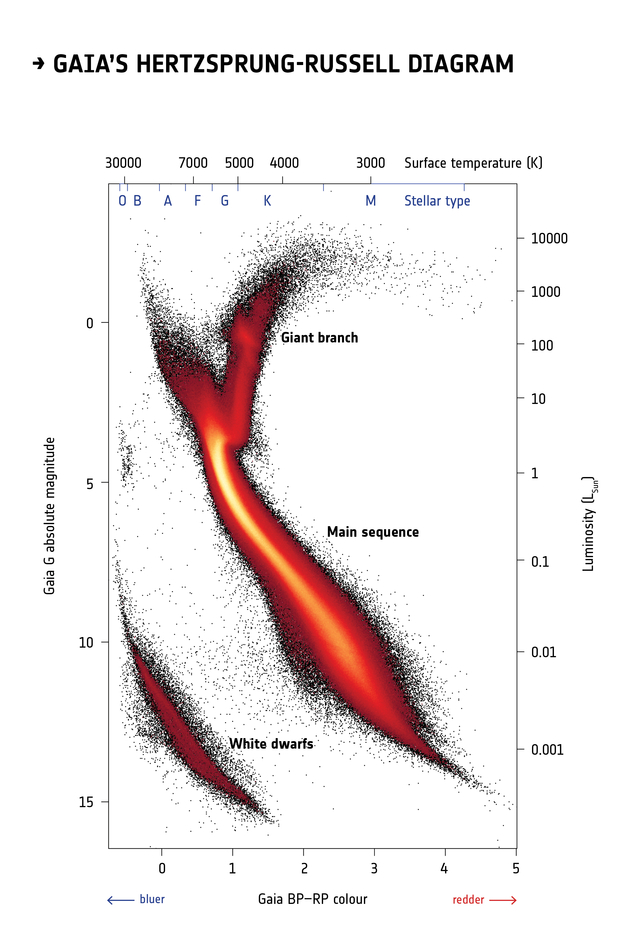
\includegraphics[height=0.65\textheight]{Problem_12/hinh1.jpg}
    \caption{Hình vẽ biểu diễn giản đồ HR của các ngôi sao được đo đạc bởi Gaia, với độ trưng năng lượng $L$ của ngôi sao tỉ lệ với độ trưng năng lượng của mặt trời 1 trên trục tung bên phải, và nhiệt độ bề mặt $T_e(\si{K})$  trên trục hoành ở phía trên.}
\end{figure}
\newpage

\begin{enumerate}
\item Xét lớp cầu khối lượng $dm$ dày $dr$, bán kính $r$, có mật độ khối lượng là $\rho$. Một ngôi sao ở trạng thái cân bằng thuỷ tĩnh khi mà lực hấp dẫn của chính nó cân bằng với nội áp suất từ bên trong ngôi sao tạo ra. Gọi áp suất tác dụng lên mặt trong lớp cầu là $p(r)$, áp suất tác dụng lên mặt ngoài lớp cầu là $p(r+dr)$. Tìm  $\dfrac{dm}{dr}$ và gradient áp suất $\dfrac{dp}{dr}$ để một ngôi sao ở trạng thái cân bằng.
\end{enumerate}
\begin{center}
    

\begin{tikzpicture}[]
    \tkzDefPoint(-3,-3){A}
    \tkzDefPoint(0,-3){D}
    \tkzDrawCircle[fill=battleshipgrey!12,thick](A,D)
    \tkzDrawPoint[color=red,thick](A)
    \tkzDefPoint(-0.8,-3){C}
    \tkzDrawCircle[fill=white,thick](A,C)
    \tkzDefPoint(-1,-3){B}
    \tkzDrawCircle[fill=battleshipgrey!12,thick](A,B)
    
    \tkzDefPointBy[rotation = center A angle 60](B)\tkzGetPoint{D}
    \tkzDrawSegment[thick,->](A,D)
    \tkzDefPointBy[rotation = center A angle 30](C)\tkzGetPoint{E}
    \tkzDrawSegment[thick,->](A,E)
    \tkzLabelSegment[above=1pt](A,D){$r$}
    \tkzLabelSegment[below=1pt,rotate=30](A,E){$r+dr$}
    \tkzDefPoint(0.5,-3){F}
    \tkzDefPoint(-0.8,-3){L}
    \tkzDrawSegment[->](F,L)
    \tkzLabelPoint[right](F){$dm$}
\end{tikzpicture}
\end{center}
Cho phân bố vật chất bên trong mặt trời:

\begin{equation}
\rho(x)=293\exp{(-10.5x)}-139\exp{(-22.7x)} ,
\end{equation}
trong đó $x=\dfrac{r}{R}$.

Áp suất tác dụng lên lớp ngoài cùng của Mặt trời đến từ sự suy giảm bức xạ photon trong quang quyển của mặt trời. Độ dày quang học là một đại lượng đặc trưng cho sự suy giảm đó. Cho biết độ dày quang học của photon là:

\begin{equation}
    \tau(R)=\int_R^\infty \kappa \rho dr =\dfrac{2}{3},
\end{equation}
với $\kappa$ có thể coi là hằng số khi $r>R$. 
\begin{enumerate}[resume]
    \item Tính áp suất $P_\text{s}$ ở bề mặt Mặt Trời, từ đó tính áp suất tại tâm Mặt Trời, biết tâm mặt trời có thể coi là $0.1\%$ bán kính.
\end{enumerate}
\begin{enumerate}[resume]
        \item Thành phần của tâm mặt trời bao gồm 74\% Hidro, 24\% Heli và 2\% các kim loại nặng khác. Tại trung tâm của ngôi sao, do nhiệt đô cao nên vật chất tồn tại ở thể plasma (vật chất bị ion hoá hoàn toàn) nên nó có khối lượng mol khoảng $\mu_i=0.62 \si{g \cdot mol^{-1}}$. Coi khí plasma là khí lý tưởng, ước tính nhiệt độ $T_\text{c}$ ở tâm mặt trời.
\end{enumerate}

Do sự chênh lệch nhiệt độ giữa tâm và bề mặt của một ngôi sao, năng lượng có xu hướng "chảy" từ trong ra ngoài thông qua bức xạ điện từ. Ta hãy xem xét lực do bức xạ tác dụng lên lớp cầu $dm$ trong trường hợp này.
Khi một bức xạ xuyên qua một môi trường truyền thì năng lượng của nó bị chất truyền dẫn đó hấp thụ một phần. Cụ thể, cường độ của bức xạ đó sau khi đi được quãng đường $x$ trong môi trường truyền có mật độ khối lượng $\rho$ và độ mờ $\kappa$ được miêu tả bằng hàm
\begin{equation}
    I(x)=I_0 \exp{(\kappa \rho x)}.
\end{equation}
\begin{enumerate}[resume]
    \item Biết năng lượng bức xạ tới lớp cầu $dr$ trong một đơn vị thời gian là $l(r)$. Tính áp suất bức xạ $dp_{\text{rad}}$ gây ra trên lớp cầu.
    
\end{enumerate}
\begin{enumerate}[resume]
    \item Cho độ mờ trung bình của mặt trời là $\langle \kappa \rangle = 10^2 \si{m^2 \cdot kg^{-1}}$. Độ trưng năng lượng Eddington là độ trưng lớn nhất có thể có của một ngôi sao. Tìm độ trưng Eddington của Mặt Trời.
\end{enumerate}
Người ta tìm thấy rằng áp suất bức xạ bằng một phần ba mật độ năng lượng bức xạ vật đen, kết hợp với định luật Stefan-Boltzmann, ta được: 
\begin{equation}
    p=\dfrac{u}{3}=\dfrac{4\sigma}{3c} T^4 = \dfrac{a}{3}T^4 ,
\end{equation} 

trong đó $a$ được gọi là hằng số bức xạ.
\begin{enumerate}[resume]
    \item Tìm quy luật phân bố nhiệt độ bên trong một ngôi sao dãy chính.   
    \item Cho năng lượng tạo ra do phản ứng hạt nhân của một ngôi sao trong một đơn vị thời gian và trên một đơn vị khối lượng là $\epsilon$. Tìm quy luật phân bố độ trưng năng lượng của một ngôi sao. Độ trưng năng lượng của một ngôi sao tỉ lệ với luỹ thừa bậc mấy của nhiệt độ ? Từ đó so sánh với giản đồ HR và nhận xét. Thời gian một ngôi sao tồn tại ở dãy chính tỉ lệ thế nào với khối lượng của nó.
\end{enumerate}


\begin{enumerate}[resume]
    
    \item Thời khắc cuối cùng của một ngôi sao ở dãy chính diễn ra khi mà Hidro bị chuyển hoá hết thành Heli. Do tốc độ phản ứng tỉ lệ với nhiệt độ, nên khi Hidro ở trong tâm bị sử dụng hết, thì ở phía ngoài, nơi nhiệt độ thấp hơn, Hidro vẫn đang được đốt cháy, tạo ra một lớp vỏ Hidro ở phía ngoài. Khi lõi Heli bên trong đạt tới khối lượng khi mà nó sụp đổ do áp suất của lớp vỏ bên ngoài, gọi là giới hạn Schönberg-Chandrasekhar thì ngôi sao bước vào giai đoạn Sao khổng lồ đỏ. Tìm giới hạn Schönberg-Chandrasekhar $\dfrac{M_\text{c}}{M}$ theo tỉ số $\dfrac{\mu_\text{c}}{\mu_\text{s}}$, với $M_\text{c}$, $M$, $\mu_\text{c}$, $\mu_\text{s}$ lần lượt là khối lượng lõi, khối lượng ngôi sao, khối lượng nguyên tử của lõi và khối lượng nguyên tử của lớp vỏ.  
\end{enumerate}

\begin{flushright}
    (Biên soạn bởi Hiagari)
\end{flushright}
\setcounter{equation}{0}
\begin{center}
    \normalcolor{\textbf{Bài giải}}
\end{center}
\begin{enumerate}
\item Xét một lớp vỏ cầu bán kính $r$ dày $dr$, khối lượng của lớp vỏ cầu này là
\begin{equation}
    dm=\rho 4 \pi r^2 dr .\label{mgrad}
\end{equation}
Do lực do áp suất gây ra cân bằng với lực hấp dẫn nên
\begin{equation}
    \dfrac{dp}{dr}= -\dfrac{Gm \rho}{r^2} .
    \label{pgrad}
\end{equation}

\item Lấy tích phân biểu thức \eqref{pgrad}, ta được
\begin{equation}
    P_\text{sur}= \int_{R}^{\infty} -\dfrac{GM\rho}{r^2} dr = \dfrac{GM}{R^2} \int_{R}^{\infty} \rho dr = \dfrac{GM}{\kappa R^2} \tau(R) =\dfrac{2GM}{3\kappa R^2}.\label{psur}
\end{equation}

Từ hàm $\rho$ thay $x=0.001$ ta tính được $\rho \approx 154 \si{g\cdot cm^{-3}}$.

Theo \eqref{pgrad}

\begin{equation}
    \dfrac{dp}{dr}= -\dfrac{GM \rho}{r^2}.\label{pcore}
\end{equation}

Thế hàm $\rho$ và tích phân ta được $p\approx 28.9 Pa$.

\item Từ phương trình khí lý tưởng

\begin{equation}
    p =\dfrac{\rho R T}{\mu} \Longrightarrow T= \dfrac{p \mu}{R \rho}.\label{tempcore}
\end{equation}


Thay số tính được $T \approx 14$ triệu độ.

\item Lực gây ra là do photon va chạm với môi trường truyền làm mất một phần động lượng và chuyển thành lực. Do góc khối phát bức xạ là như nhau nên $I\sim E$
\begin{equation}
    \Delta F_r =\dfrac{dp}{dt} = \dfrac{dE}{cdt}=\dfrac{l}{c} = \dfrac{l_0 [1-\exp{(\kappa \rho \Delta r)} ] }{c} \approx -\dfrac{l(r)}{c} \kappa \rho \Delta r \Longrightarrow dF_r = -\dfrac{l(r)}{c} \kappa \rho dr.\label{dfrad}
\end{equation}
\item Từ $dF_r$ vừa tìm được ở trên, chúng ta có thể tìm gradient áp suất trên tại bề mặt, kết hợp với điều kiện cân bằng thuỷ tĩnh \eqref{pgrad}, ta tìm được
\begin{equation}
    L_{Ed}=\dfrac{4\pi Gc}{\langle \kappa \rangle} M.\label{leddington}
\end{equation}
\item Thông qua áp suất bức xạ ta có

\begin{equation}
    dF_r =4\pi r^2 dp =4 \pi r^2 \dfrac{4aT^3}{3}dT =\dfrac{16a\pi r^2 T^3}{3}dT.
\end{equation}

Từ 2 phương trình trên ta có

\begin{equation}
    dF_r=\dfrac{16a\pi r^2 T^3}{3}dT=-\dfrac{l(r)}{c} \kappa \rho dr \Longrightarrow l(r) = -\dfrac{16ca\pi r^2 T^3}{3\kappa \rho}\dfrac{dT}{dr}. \label{eq_9_12}
\end{equation}

\item Ta tìm được gradient độ trưng năng lượng từ định nghĩa
\begin{equation}
    \dfrac{dl(r)}{dr}=4\pi r^2 \rho \varepsilon.\label{eq_10_12}
\end{equation}

Xuất phát từ \eqref{pgrad}
\begin{equation}
    \begin{split}
    \dfrac{dp}{dr}&= -\dfrac{GM \rho}{r^2}.
\end{split}
\end{equation}

Lưu ý rằng $\rho \sim \dfrac{M}{R^3}$.

Ta được

\begin{equation}
    p \sim -\dfrac{M^2}{R^4}.
\end{equation}

Từ phương trình khí lý tưởng ta có $p \sim \rho T$.

Ta được 
\begin{equation}
    T \sim M/R.
\end{equation}

Từ $l(r)=-\dfrac{16ca\pi r^2 T^3}{3\kappa \rho}\dfrac{dT}{dr}$ tìm được

\begin{equation}
    L \sim M^3.\label{eq_14_12}
\end{equation}

Từ định luật Stefan-Boltzmann $L=4\pi r^2 \sigma T^2_e$ ta được
\begin{equation}
    L \sim R^2T^4 = (TR)^2T^2 \Rightarrow M^3 \sim M^2T^2 \Rightarrow M \sim T^2. 
\end{equation}


Vậy $L \sim T^6$ và $\tau \sim M^{-2}$.

8. Từ điều kiện cân bằng thuỷ tĩnh
\begin{equation}
    \dfrac{dp}{dm}=-\dfrac{Gm}{4\pi r^4} \Rightarrow 4\pi r^3\dfrac{dp}{dm}=-\dfrac{Gm}{r}.
\end{equation}
Xét vế trái, sử dụng phương trình khối lượng
\begin{equation}
    4\pi r^3\dfrac{dp}{dm} =\dfrac{d(4\pi r^3 p)}{dm}-12\pi r^2 p\dfrac{dr}{dm} =\dfrac{d(4\pi r^3 p)}{dm}-\dfrac{3p}{\rho}.\label{eq_17_12}
\end{equation}
Tích phân phương trình 1 trên toàn bộ khối lượng lõi Heli
\begin{equation}
    \int_0^{M_c}\dfrac{d(4\pi r^3 p)}{dm}dm-\int_0^{M_c}\dfrac{3p}{\rho}dm=\int_0^{M_c}-\dfrac{Gm}{r}dm.
    \label{cdh}
\end{equation}
Từ phương trình khí lí tưởng $\dfrac{P}{\rho}=\dfrac{RT}{\mu}$, do lõi Heli đẳng nhiệt nên
\begin{equation}
    \int_0^{M_c}\dfrac{3p}{\rho}dm = \dfrac{3M_cRT_c}{\mu_c}=2U_c ,
\end{equation}
ở đó $K_c$ là nội năng của khí He trong lõi.

Thành phần bên trái phương trình \eqref{cdh} là thế năng hấp dẫn của lõi
\begin{equation}
    \int_0^{M_c}-\dfrac{Gm}{r}dm = -\frac35 \dfrac{GM^2_c}{R_c}.\label{eq_20_12}
\end{equation}
Thế vào phương trình \eqref{cdh} và hoàn thành tích phân còn lại, ta được
\begin{equation}
    4\pi R^3_cP_c-3 \dfrac{M_cRT_c}{\mu_c}=-\frac35 \dfrac{GM_c^2}{R_c} \Longrightarrow P_c=\dfrac{3}{4\pi R^3_c}\left(\dfrac{M_cRT_c}{\mu_c}-\frac15 \dfrac{GM^2_c}{R_c}\right).
\end{equation}
Từ phương trình trên, với giá trị $R_c$ xác định, ta thấy rằng khi khối lượng lõi tăng lên thì năng lượng nhiệt sẽ tăng áp suất ở bề mặt của lõi, trong khi thế năng hấp dẫn gây giảm áp suất. Ta tìm được áp suất lớn nhất trên bề mặt lõi
\begin{equation}
    P_{c,max} = \dfrac{375}{64\pi}\dfrac{1}{G^3M_c^2}\left(\dfrac{RT_c}{\mu_c}\right)^4 .\label{eq_22_12}
\end{equation}

Dễ dàng thấy được khi $M_c$ tăng thì áp suất trên giảm. Do đó, ở một giá trị khối lượng của lõi, cân bằng thuỷ tĩnh sẽ bị phá vỡ.

Chúng ta sẽ tìm áp suất tác dụng lên bề mặt lõi bởi lớp vỏ.
Từ điều kiện cân bằng thuỷ tĩnh
\begin{equation}
    \dfrac{dp}{dm}=-\dfrac{Gm}{4\pi r^4} \Longrightarrow P_s \approx \dfrac{G}{8\pi\langle r^4 \rangle} (M^2-M_c^2) \approx \dfrac{G}{4\pi} \dfrac{M^2}{R^4} .
\end{equation}
Thông qua $\rho_s$ và phương trình khí lí tưởng, ta tìm được:
\begin{equation}
    P_s \approx \dfrac{81}{4\pi}\dfrac{1}{G^3M^3}\left(\dfrac{RT_c}{\mu_s}\right)^4 .\label{eq_24_12}
\end{equation}
Như vậy, ta tìm được giới hạn S-C khi mà lõi còn có thể duy trì được cân bằng thuỷ tĩnh:
\begin{equation}
    \dfrac{M_c}{M} \approx 0.537 \left(\dfrac{\mu_s}{\mu_c}\right)^2 .\label{eq_25_12}
\end{equation}

\end{enumerate}
\textbf{Biểu điểm}
\begin{center}
\begin{tabular}{|>{\centering\arraybackslash}m{1cm}|>{\raggedright\arraybackslash}m{14cm}| >{\centering\arraybackslash}m{1cm}|}
    \hline
    \textbf{Phần} & \textbf{Nội dung} & \textbf{Điểm} \\
    \hline
    \textbf{1} & Tìm được gradient khối lượng \eqref{mgrad} & $0.50$ \\
    \cline{2-3}
    & Tìm được gradient áp suất \eqref{pgrad} & $0.50$ \\
    \hline
    \textbf{2} & Tìm được áp suất bề mặt \eqref{psur} & $0.50$ \\
    \cline{2-3}
    & Tìm được áp suất tại tâm \eqref{pcore} & $0.50$ \\
    \hline
    \textbf{3} & Tìm được nhiệt độ tại tâm \eqref{tempcore} & $0.50$ \\
    \hline
    \textbf{4} & Dẫn ra được lực do áp suất bức xạ gây ra trên lớp cầu \eqref{dfrad} & $0.50$ \\
    \hline
    \textbf{5}
    & Tìm được độ trưng Eddington của Mặt Trời \eqref{leddington} & $0.50$ \\
    \hline
    \textbf{6}
    & Tìm ra được hàm độ trưng năng lượng \eqref{eq_9_12} & $0.50$ \\ 
    \hline
    \textbf{7}
    & Tìm ra được hàm độ trưng năng lượng theo định nghĩa \eqref{eq_10_12} & $0.50$ \\
    \cline{2-3}
    & Tìm ra được quan hệ tỉ lệ giữa $L$ và $M$ & $0.50$\\
    \cline{2-3}
    & Tìm ra được quan hệ tỉ lệ giữa $L$ và $T$ và giữa $\tau$ và $M$ & $0.50$\\
    \hline
    \textbf{8}
    & Dẫn ra được phương trình \eqref{eq_17_12} & $0.50$ \\
    \cline{2-3}
    & Tính được thế năng hấp dẫn của lõi \eqref{eq_20_12} & $0.50$\\
    \cline{2-3}
    & Tìm ra được áp suất lớn nhất trên bề mặt lõi \eqref{eq_22_12} & $0.50$\\
    \cline{2-3}
    & Tìm ra được áp suất tác dụng lên bề mặt lõi bởi lớp vỏ ngoài \eqref{eq_24_12} & $0.50$\\
    \cline{2-3}
    & Tìm ra được giới hạn S-C \eqref{eq_25_12} & $0.50$\\
    
    
    \hline
\end{tabular}
\end{center}  


\bibliographystyle{plain}
\begin{thebibliography}{}
\bibitem{JphO} \href{http://www.jpho.jp/syllabus.html}{JPhO 2022 Theory Problems}.
\bibitem{carroll} Bradley W.Carroll, Dale A.Ostlie. \textit{An Introduction to Modern Astrophysics}
\end{thebibliography}




\newpage
{\normalcolor \textbf{CÂU 13 (8 điểm)}}\vspace{1.5mm}

\setcounter{equation}{0}
%%Bài toán đề xuất bởi NVPL

\textbf{Tương tác tĩnh điện của protein}

Nghiên cứu về vật lý trong sinh học đã trở thành một trong những chủ đề bùng nổ và hấp dẫn gần đây, trong số đó có chủ đề mà bài toán này tìm hiểu, đó là tương tác tĩnh điện của protein trong DNA với điện tích trong môi trường nước hoặc trong môi trường có ion tự do (môi trường chứa muối đơn trị như NaCl) để giải thích một số quá trình như \textit{đảo điện tích (charge inversion)} trong hệ thống polyelectrolyte-micelle hay trên bề mặt rắn của màng mica hoặc lipid; hay hiện tượng \textit{điện di (electrophoresis)} trong quá trình sinh học (Ví dụ như quá trình chuyển gen đến tế bào sống với mục đích trị liệu gen,...).

\begin{enumerate}
    \item \textbf{Axit amin trong protein.} \\
    Đầu tiên ta tìm hiểu tại sao sâu bên trong protein, axit amin ion hoá lại hầu như không tích điện. Ta xét mô hình đơn giản của một điện tích, giả thiết như một quả cầu bán kính $R\approx 1.5\ \si{\angstrom}$, tích điện $q=\text{e}\approx 1.6 \times 10^{-19}\ \si{C} $, di chuyển từ môi trường nước bên ngoài protein vào sâu bên trong protein. Protein và nước coi như môi trường điện môi đồng nhất với hằng số điện môi lần lượt là $\epsilon_p \approx 3$, $\epsilon_w \approx 80$. Cho biết năng lượng tĩnh điện cần để phá huỷ bất kỳ cấu trúc protein nào xấp xỉ $E_0 \approx 5\ \si{kcal/mol}$ $(1\ \si{J} \approx 1.44 \times 10^{20}\ \si{kcal/mol})$.\\ \textit{Lưu ý: Trong toàn bộ bài tập này ta sẽ chủ yếu dùng đơn vị $\si{kcal/mol}$ cho năng lượng vì trong nghiên cứu về tế bào chủ yếu sử dụng đơn vị này nhưng vẫn chấp nhận kết quả bằng đơn vị Joule.}\\ \\
    Xác định độ chênh lệch năng lượng tĩnh điện của một điện tích nếu điện tích đó xuất hiện bên trong protein. Vậy tại sao axit amin ion hoá lại hầu như không tích điện bên trong protein ?

    \item \textbf{Tương tác giữa điện tích và protein trong môi trường nước.} \\
    \begin{center}
    \begin{figure}[htp]
    \begin{center}
        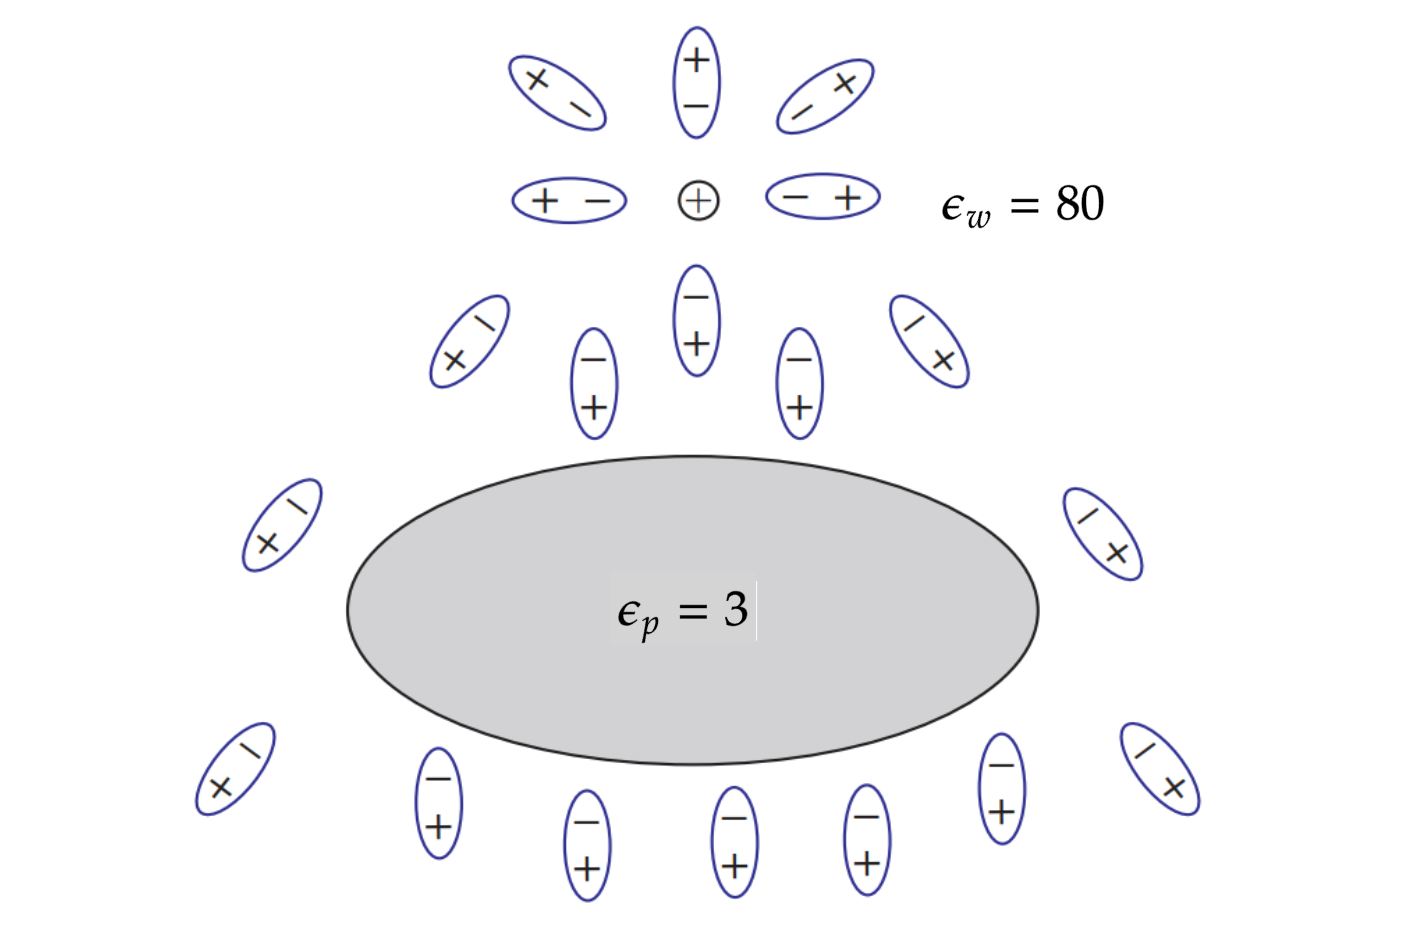
\includegraphics[scale=.23
        ]{Problem_13/image/1.png}
    \end{center}
    \begin{center}
    Hình 1: Các lưỡng cực bị phân cực
    \end{center}
    \end{figure}
\end{center}
    Tiếp đến ta tính tương tác của các điện tích ở gần hay tại mặt phân cách của protein và nước \textbf{(Hình 1)}. Coi điện tích rất bé và nằm rất gần so với protein để có thể mô hình hoá protein như một tấm điện môi đồng nhất có hai mặt phẳng rộng vô hạn song song với nhau \textbf{(Hình 2)}. Trong từng vùng môi trường, tồn tại "hằng số điện môi hiệu dụng" $\epsilon_{\text{eff}}$, cho phép tính điện thế của điện tích $q$ gây ra tại vị trí $\Vec{r}$ rất xa so với chính nó (nhưng đủ lớn để không coi điện thế bằng $0$) như thể điện tích $q$ được đặt trong môi trường điện môi đồng nhất có hằng số điện môi bằng hằng số điện môi hiệu dụng:$$V(\Vec{r})=\dfrac{kq^2}{\epsilon_{\text{eff}}\left|\Vec{r}\right|}.$$ Do vùng không gian môi trường nước chứa điện tích, các lưỡng cực phân cực mạnh hơn vùng không gian không chứa điện tích nên khi ta khảo sát tương tác tĩnh điện đối với mặt phân cách gần điện tích thì ảnh hưởng của mặt phân cách xa điện tích là không đáng kể. Ngoài ra khi khảo sát tĩnh điện ở vùng không gian môi trường nước không chứa điện tích, các lưỡng cực trong nước bị phân cực mạnh hơn trong protein nên ta chỉ xét ảnh hưởng của các điện tích liên kết trong môi trường nước ở mặt phân cách xa điện tích. Do đó ta gần đúng hệ này bằng cách tách thành hai hệ tương tác tĩnh điện giữa điện tích điểm $q$ hoặc $q''$ và mặt phẳng điện môi bán vô hạn \textbf{(Hình 2)}.
    \begin{center}
    \begin{figure}[htp]
    \begin{center}
        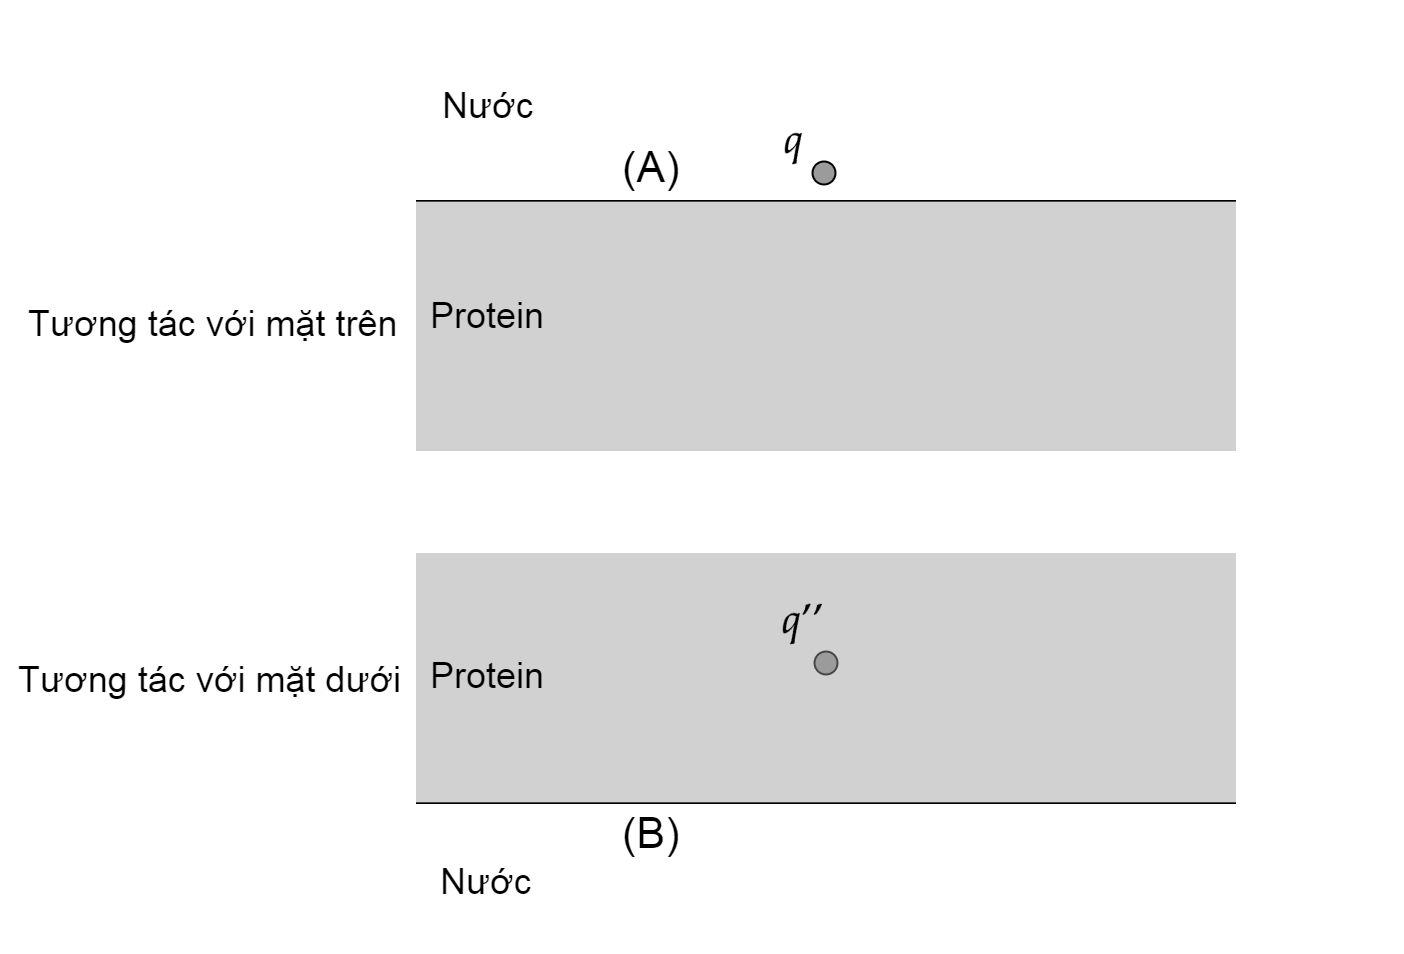
\includegraphics[scale=.27
        ]{Problem_13/image/2.png}
    \end{center}
    \begin{center}
    Hình 2: Tương tác giữa điện tích và protein trong từng môi trường. Điện tích $q$ là điện tích ban đầu ta xét. Điện tích $q''$ là điện tích ảnh sinh ra do sự tương tự về mặt tĩnh điện của các điện tích liên kết trong môi trường protein.
    \end{center}
    \end{figure}
\end{center}

     \begin{enumerate}[label=\textbf{\alph*,}]\itemsep0em
        \item Xác định hằng số điện môi hiệu dụng trong vùng môi trường nước chứa điện tích.
        \item Xác định hằng số điện môi hiệu dụng trong vùng môi trường bên trong protein.
        \item Xác định hằng số điện môi hiệu dụng trong vùng môi trường nước không chứa chứa điện tích.
    \end{enumerate}

    \item \textbf{Tương tác giữa điện tích và protein trong môi trường có ion tự do.} \\ 
    Cho đến giờ ta mới chỉ tìm hiểu về tương tác giữa các điện tích riêng biệt. Tuy nhiên ta đã "bỏ sót" tương tác của các lưỡng cực (các lưỡng cực cũng tham gia vào liên kết hydro như $\text{H}^+ - \text{O}^-$ và $\text{H}^+ - \text{N}^-$) và cũng như các tứ cực (các vòng thơm) bên trong các cấu trúc tế bào. Thêm vào đó, do các điện tích tự do có sẵn trong nước (nước muối), từ những điều kể trên chúng ta rút ra biểu thức điện thế gây ra bởi điện tích $q$ tại vị trí $\Vec{r}$ rất xa so với chính nó (nhưng đủ lớn để không coi điện thế bằng $0$) có dạng: $$V(r)=\dfrac{kq}{\epsilon_{\text{eff}}}\dfrac{e^{-r/D}}{r}.$$Thế năng này gọi là thế "chắn" hay thế Debye-Huckel hay thế Yukawa, xuất hiện rất nhiều trong các lĩnh vực khác nhau của vật lý. Ở đây $D$ là bán kính "chắn" Debye-Huckel, tương ứng với kích thước điển hình của đám mây phản ion xung quanh điện tích. Giá trị của $D$ không phụ thuộc vào điện tích $q$ mà phụ thuộc hằng số điện môi hiệu dụng, nhiệt độ và cường độ ion (ionic strength) $I\ \si{mol/l}$ của dung dịch: $$I=\dfrac{1}{2}\sum\limits_i {{c_i}N_i^2}. $$ Trong đó $N_i$ là tỉ số giữa điện tích của ion loại $i\ (i=1,2,3,...)$ và điện tích nguyên tố. $c_i$ là nồng độ của ion loại $i$, tính bằng $\si{mol/l}$. Cho biết mật độ điện tích ion trong môi trường tuân theo phân bố Maxwell- Boltzmann: $$\rho(r)=\sum\limits_i {{c_i}\left( {\text{e}{N_i}} \right)} {e^{ - E_i/(k_BT)}}.$$ Giả thiết $E_i \ll k_BT$ ($T$ là nhiệt độ, $k_B$ là hằng số Boltzmann) và các ion coi như đứng yên. Hệ ion coi là trung hoà. Cho biết toàn bộ hệ ở nhiệt độ phòng $T=20 \si{^\circ C}$, hằng số điện môi hiệu dụng $\epsilon_{\text{eff}}=40$, cường độ ion $I \approx 0.12\ \si{mol/l}$. \\ \\
    Hãy xác định bán kính chắn Debye-Huckel của hệ.\\ \\
\textit{Có thể bạn cần dùng: $\nabla_r f(r)=\dfrac{1}{r}\dfrac{\partial}{\partial r}\Big(rf(r)\Big).$}


    
\end{enumerate}
\begin{flushright}
    (Biên soạn bởi Nhân viên phòng lab)
\end{flushright}
\setcounter{equation}{0}
\begin{center}
    \normalcolor{\textbf{Bài giải}}
\end{center}
\begin{enumerate}
    \item \textbf{Axit amin trong protein.} \\
    Mật độ năng lượng điện trường trong môi trường $\epsilon$ bất kỳ:
\begin{equation} \label{eq1_Protein}
    \omega = \dfrac{1}{2}\epsilon\epsilon_0E^2 = \dfrac{kq^2}{8\pi\epsilon k  r^4}.
\end{equation}
Năng lượng tĩnh điện trong môi trường $\epsilon$ bất kỳ:
\begin{equation} \label{eq2_Protein}
    W =\displaystyle\int\limits^{\infty}_{R}\omega 4\pi r^2dr=\displaystyle\int\limits^{\infty}_{R}\dfrac{kq^2}{2\epsilon r^2}dr  =\dfrac{kq^2}{2\epsilon R}.
\end{equation}
Thay số:
\begin{align} 
    \label{eq3_Protein}
    W_p&\approx 2.56 \times 10^{-19} \ \si{J} \approx 36.86 \ \si{kcal/mol},\\
    \label{eq4_Protein}
    W_w&\approx 9.61 \times 10^{-21} \ \si{J} \approx 1.38 \ \si{kcal/mol}.
\end{align}
Độ chênh lệch năng lượng:
\begin{equation} \label{eq5_Protein}
    \Delta W = |W_w - W_p| = 35.48 \ \si{kcal/mol}.
\end{equation}
Như vậy độ chênh năng lượng tĩnh điện khi điện tích đi từ nước vào protein hay chính bằng năng lượng cung cấp cho cấu trúc protein sẽ rất lớn so với năng lượng cần để phá huỷ cấu trúc protein, vì vậy bên trong protein hầu như axit amin không tích điện để không phá huỷ cấu trúc protein. \\
\textit{Trên thực tế, vẫn có các cấu trúc phân tử tích điện xuất hiện bên trong protein nhưng các phân tử này đóng vai trò của các nhóm chức năng và tham gia các hoạt động sinh học của protein chứ không phải nhóm cấu tạo nên không làm phá huỷ cấu trúc protein.}
     \item \textbf{Tương tác giữa điện tích và protein trong môi trường nước.}
     \begin{enumerate}[label=\textbf{\alph*,}]\itemsep0em
         \item Ta sử dụng phương pháp ảnh điện. Giả sử ban đầu điện tích $q$ có toạ độ $\Vec{r}_0$ ($R\ll|\Vec{r}_0| \ll |\Vec{r}|$) với gốc là một điểm nằm trên mặt phân cách $(A)$ \textbf{(Hình 3)}. Để thoả mãn điều kiện biên của điện trường tại mọi điểm trên mặt phân cách $(A)$, hệ tương đương như sau:
         \begin{enumerate}
             \item Điện tích ảnh $q'=\dfrac{\epsilon_w-\epsilon_p}{\epsilon_w+\epsilon_p}q$ của điện tích $q$ qua mặt $(A)$, trong môi trường nước, đặt tại $\Vec{r}_1=-\Vec{r}_0$.
             \item Điện tích ảnh $q''=\dfrac{2\epsilon_p}{\epsilon_w+\epsilon_p}q$ của điện tích $q'$ qua mặt $(A)$, trong môi trường protein, đặt tại $\Vec{r}_2=\Vec{r}_0$.
         \end{enumerate}
\begin{center}
    \begin{figure}[htp]
    \begin{center}
        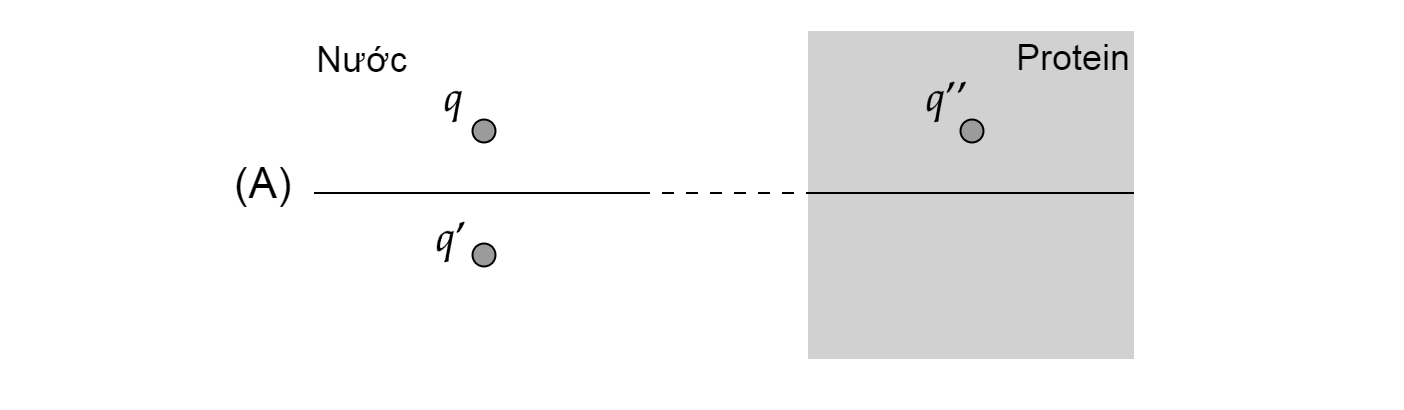
\includegraphics[scale=.27
        ]{Problem_13/image/3.png}
    \end{center}
    \begin{center}
    Hình 3: Điện tích $q$ và các điện tích ảnh tương ứng.
    \end{center}
    \end{figure}
\end{center}
         Điện tích $q$ và $q'$ tham gia vào tương tác tĩnh điện trong vùng môi trường nước chứa điện tích, $q''$ tham gia vào vùng môi trường protein. Thế năng tĩnh điện trong từng vùng môi trường:
\begin{align}
    \label{eq6_Protein}
    V_{\text{nước}\uparrow}&=\dfrac{kq}{\epsilon_w \left|\Vec{r}-\Vec{r}_0\right|}+\dfrac{kq'}{\epsilon_w \left|\Vec{r}-\Vec{r}_1\right|} \approx \dfrac{k(q+q')}{\epsilon_w r}=\dfrac{2kq}{(\epsilon_w+\epsilon_p) r}, \\
    \label{eq7_Protein}
    V_{\text{protein}}&=\dfrac{kq''}{\epsilon_p \left|\Vec{r}-\Vec{r}_2\right|} \approx \dfrac{kq''}{\epsilon_p r}=\dfrac{2kq}{(\epsilon_w+\epsilon_p) r}.
\end{align}
Từ phương trình (\ref{eq6_Protein}) ta suy ra hằng số điện môi hiệu dụng tương ứng với vùng môi trường nước chứa điện tích:
\begin{equation} \label{eq8_Protein}
    \epsilon_{\text{eff}}^{(1)}=\dfrac{\epsilon_w+\epsilon_p}{2}=41.50.
\end{equation}
          \item  Từ phương trình (\ref{eq7_Protein}) ta suy ra hằng số điện môi hiệu dụng tương ứng với vùng môi trường bên trong protein:
\begin{equation} \label{eq9_Protein}
    \epsilon_{\text{eff}}^{(2)}=\dfrac{\epsilon_w+\epsilon_p}{2}=41.50.
\end{equation}
          \item Do khi khảo sát tĩnh điện ở vùng không gian môi trường nước không chứa điện tích, các lưỡng cực trong nước bị phân cực mạnh hơn trong protein nên ta chỉ xét ảnh hưởng của các điện tích liên kết trong môi trường nước ở mặt phân cách xa điện tích $q$ nên điện tích tham gia vào tương tác chỉ có điện tích ảnh sinh ra do các điện tích liên kết trong môi trường nước hình thành ở mặt phân cách xa điện tích $q$. Điện tích này tương tự điện tích ảnh $q''$ đối với chính $q''$, ta gọi là $q'''$ \textbf{(Hình 4)}. Điện tích ảnh $q'''=\dfrac{2\epsilon_w}{\epsilon_p+\epsilon_w}q''=\dfrac{4\epsilon_w\epsilon_p}{(\epsilon_w+\epsilon_p)^2}q$ của điện tích $q''$ qua mặt $(B)$, trong môi trường nước, đặt tại $\Vec{r}_3$.\\
\begin{center}
    \begin{figure}[htp]
    \begin{center}
        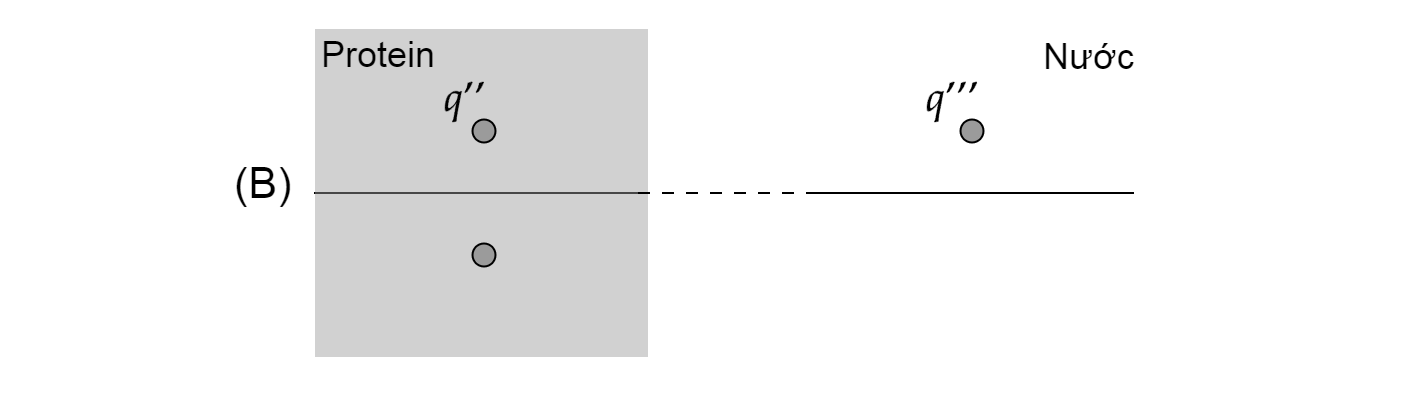
\includegraphics[scale=.27
        ]{Problem_13/image/4.png}
    \end{center}
    \begin{center}
    Hình 4: Điện tích $q''$ và điện tích ảnh $q'''$.
    \end{center}
    \end{figure}
\end{center}
          Thế năng tĩnh điện trong vùng môi trường nước không chứa điện tích:
          \begin{equation} \label{eq10_Protein}
              V_{\text{nước}\downarrow}=\dfrac{kq'''}{\epsilon_w \left|\Vec{r}-\Vec{r}_3\right|} \approx \dfrac{kq'''}{\epsilon_w r}=\dfrac{4\epsilon_p kq}{(\epsilon_w+\epsilon_p)^2 r}.
          \end{equation}
          Từ phương trình (\ref{eq10_Protein}) ta suy ra hằng số điện môi hiệu dụng tương ứng với vùng môi trường nước không chứa điện tích:
          \begin{equation} \label{eq11_Protein}
          \epsilon_{\text{eff}}^{(3)}=\dfrac{(\epsilon_w+\epsilon_p)^2}{4\epsilon_p}\approx 574.08.
          \end{equation}
     \end{enumerate}
     \textit{Kết quả thực nghiệm cho kết quả (11) chỉ cỡ 200, giải thích cho điều này là do kích thước của protein hữu hạn nên gần đúng chúng ta sử dụng trong bài tương đối cực đoan, nhưng dù sao 200 vẫn là con số khá lớn so với 41,5. Các thí nghiệm bởi nhóm nghiên cứu của Alan Fersht cho thấy những ước tính trên cũng phù hợp với protein. Trong các thí nghiệm của Fersht, các đột biến được thực hiện trên bề mặt của protein để không làm hỏng cấu trúc của nó. Kết quả thực nghiệm cho thấy: hằng số điện môi hiệu dụng nằm trong khoảng từ 40 đến 200. Thực tế là $\epsilon_{\text{eff}}$ có thể đạt đến giá trị 200 không có gì đáng ngạc nhiên sau các xem xét chúng ta đã thực hiện ở trên. Phương pháp ảnh điện phổ thông đã mô tả và giải thích khá thành công cho một số hiện tượng vật lý trong sinh học (Bạn có thể tham khảo một số công trình khoa học của GS. TS Nguyễn Thế Toàn về vật lý sinh).}
     \item \textbf{Tương tác giữa điện tích và protein trong môi trường có ion tự do.} \\ 
     Phương trình Poisson:
\begin{equation} \label{eq12_Protein}
    \nabla^2_r V(r) = - \dfrac{4\pi k \rho}{\epsilon_{\text{eff}}} = - \dfrac{4\pi k \text{e}}{\epsilon_{\text{eff}}}\sum\limits_i {{c_i}{N_i}} {e^{ - E_i/k_BT}} \approx - \dfrac{4\pi k \text{e}}{\epsilon_{\text{eff}}}\sum\limits_i {{c_i}{N_i}}\left(1- \dfrac{E_i}{k_BT}\right).
\end{equation}
Năng lượng của ion loại $i$:
\begin{equation} \label{eq13_Protein}
    E_i=\text{e}N_iV(r).
\end{equation}
Thay phương trình (\ref{eq13_Protein}) vào phương trình (\ref{eq12_Protein}):
\begin{equation} \label{eq14_Protein}
    \nabla^2_r V(r) =  \dfrac{4\pi k \text{e}}{\epsilon_{\text{eff}}}\sum\limits_i {{c_i}{N_i}} \left(\dfrac{\text{e}N_iV(r)}{k_BT}-1 \right)=\dfrac{8\pi k \text{e}^2 V(r)}{\epsilon_{\text{eff}}k_BT}\sum\limits_i \dfrac{1}{2}{{c_i}{N_i^2}} - \dfrac{4\pi k \text{e}}{\epsilon_{\text{eff}}}\sum\limits_i {{c_i}{N_i}}.
\end{equation}
Do hệ ion trung hoà nên $\sum\limits_i {{c_i}{\text{e}N_i}}=0$, phương trình (\ref{eq14_Protein}) trở thành:
\begin{equation} \label{eq15_Protein}
    \nabla^2_r V(r)=\dfrac{8\pi k \text{e}^2 V(r)}{\epsilon_{\text{eff}}k_BT}I.
\end{equation}
Mặt khác, theo đề bài, $V(r)=\dfrac{kq}{\epsilon_{\text{eff}}}\dfrac{e^{-r/D}}{r}$, thay vào vế trái phương trình (\ref{eq15_Protein}) ta được:
\begin{equation} \label{eq16_Protein}
    \nabla^2_r V(r)=\dfrac{1}{D^2} V(r).
\end{equation}
Từ phương trình (\ref{eq15_Protein}) và phương trình (\ref{eq16_Protein}) ta suy ra:
\begin{equation} \label{eq17_Protein}
    \dfrac{1}{D^2}=\dfrac{8\pi k \text{e}^2 I}{\epsilon_{\text{eff}}k_BT} \Rightarrow 
    D= \sqrt{\dfrac{\epsilon_{\text{eff}}k_BT}{8\pi k \text{e}^2 I}}.
\end{equation}
Thay số: $D\approx 6.21\times 10^{-10}\ \si{m} = 6.21\ \si{\angstrom}$.\\
\textit{Qua bài tập này, ta thấy được một tính chất rất quan trọng trong nghiên cứu về tế bào, đó là tương tác tĩnh điện không chỉ phụ thuộc vào khoảng cách và điện tích, mà còn phụ thuộc cả đặc tính của môi trường như nhiệt độ, nồng độ ion, thậm chí còn phụ thuộc cả vào hình dạng của vật thể tương tác do hằng số điện môi hiệu dụng phụ thuộc vào hình dạng của vật.}
\end{enumerate}

\textbf{Biểu điểm}
\begin{center}
\begin{tabular}{|>{\centering\arraybackslash}m{1cm}|>{\raggedright\arraybackslash}m{14cm}| >{\centering\arraybackslash}m{1cm}|}
    \hline
    \textbf{Phần} & \textbf{Nội dung} & \textbf{Điểm} \\
    \hline
    \textbf{1} & Viết biểu thức năng lượng tĩnh điện trong môi trường $\epsilon$ (\ref{eq2_Protein}) & $0.50$ \\
    \cline{2-3}
    &  Tính được độ chênh lệch năng lượng giữa môi trường nước và môi trường protein (\ref{eq5_Protein}) & $0.50$ \\
    \cline{2-3}
    &  Lập luận và kết luận & $0.50$ \\
    \hline
    \textbf{2a} & Chỉ ra điện tích ảnh $q'$ & $0.50$ \\
    \cline{2-3}
     & Chỉ ra điện tích ảnh $q''$ & $0.50$ \\
    \cline{2-3}
    & Viết biểu thức năng lượng tĩnh điện trong vùng môi trường nước chứa điện tích $q$ (\ref{eq6_Protein}) & $0.50$ \\
    \cline{2-3}
    & Viết biểu thức năng lượng tĩnh điện trong vùng môi trường protein $q$ (\ref{eq7_Protein}) & $0.50$ \\
    \cline{2-3}
    & Tính được hằng số điện môi $\epsilon_{\text{eff}}^{(1)}$ (\ref{eq8_Protein}) & $0.50$ \\
    \hline
    \textbf{2b} & Tính được hằng số điện môi $\epsilon_{\text{eff}}^{(2)}$ (\ref{eq9_Protein}) & $0.50$ \\
    \hline
    \textbf{2c} & Chỉ ra điện tích ảnh $q'''$ & $0.50$ \\
    \cline{2-3}
    & Viết biểu thức năng lượng tĩnh điện trong vùng môi trường nước chứa điện tích $q$ (\ref{eq10_Protein}) & $0.50$ \\
    \cline{2-3}
    & Tính được hằng số điện môi $\epsilon_{\text{eff}}^{(3)}$ (\ref{eq11_Protein}) & $0.50$ \\
    \hline
    \textbf{3} & Dẫn ra phương trình Poisson (\ref{eq12_Protein}) & $0.50$ \\
    \cline{2-3}
    & Gần đúng phương trình Poisson và thu được phương trình (\ref{eq15_Protein}) & $0.50$ \\
    \cline{2-3}
    & Dẫn ra phương trình (\ref{eq16_Protein}) & $0.50$ \\
    \cline{2-3}
    & Viết biểu thức cho bán kính chắn Debye-Huckel và thay số (\ref{eq17_Protein}) & $0.50$ \\
    \hline
\end{tabular}
\end{center}

%% Reference %%
\bibliographystyle{plain}
\begin{thebibliography}{}
\bibitem{ttn2000} T. T. Nguyen, A. Yu. Grosberg, B. I. Shklovskii (2000), \textit{Macroions in Salty Water with Multivalent Ions: Giant Inversion of Charge}, Physical Review Letters, Volume 85, Issue 7, Pages 1568-1571.
\bibitem{fersht1989} Alan R. Fersht, Michael J. E. Sternberg (1989), \textit{Can a simple function for the dielectric response model electrostatic effects in globular proteins?}, Protein Engineering, vol.2 no.15 pp.527-530.
\bibitem{ladau1980} L. D. Landau, E. M. Lifshitz (1980), \textit{Statical Physics}.
\bibitem{finkelstein1964} Alexi V. Finkelstein, Oleg Ptitsyn (1964), \textit{Protein Physics: A course of lectures}.
\bibitem{Toan2021} Nguyễn Thế Toàn, Nguyễn Hoạ Mi (2021), \textit{Giáo trình Vật lý Sinh học của Protein}, NXB ĐHQGHN.
\bibitem{brooks1987} Charles L. Brooks III, Martin Karplus, B. Montgomery Pettitt (1987), \textit{Proteins: A Theoretical Perspective of Dynamics, Structure, and Thermodynamics}.
\end{thebibliography}

% \newpage
% {\normalcolor \textbf{CÂU 14}}\vspace{1.5mm}

% \setcounter{equation}{0}
% \input{Problem_14/P14}
% \setcounter{equation}{0}
% \begin{center}
%     \normalcolor{\textbf{Bài giải}}
% \end{center}
% \input{Problem_14/S14}

\newpage
{\normalcolor \textbf{CÂU 14+15 (16 điểm)}}\vspace{1.5mm}

\setcounter{equation}{0}
%%Bài toán đề xuất bởi NVPL

\textbf{Rối lượng tử}

Trong Vật Lý lượng tử, phép đo có thể làm thay đổi trạng thái của hệ cần quan sát, dẫn tới sự xuất hiện của tính xác suất trong kết quả thu được. Một hệ quả vô cùng thú vị đến từ tính chất này là khi chúng ta thực hiện đo đạc trên những hạt ở rất xa nhau thì kết quả thu được vẫn có thể liên hệ thống kê với nhau như những sự kiện xảy ra không độc lập, nếu chúng đã {\it rối lượng tử} với nhau. Theo lý thuyết, điều này khả dĩ ngay cả khi vận tốc ánh sáng là không đủ nhanh để truyền tín hiệu giữa chúng. \\
Hiện tượng {\it rối lượng tử} không tồn tại trong Vật Lý cổ điển, rất kỳ lạ và trái ngược trực giác, nên đã tạo ra những bất đồng về diễn giải thế giới lượng tử. Nổi tiếng nhất là cuộc tranh luận giữa những nhà Vật Lý được dẫn dắt bởi Niels Bohr và Albert Einstein, về vấn đề tồn tại hay không một {\it biến số ẩn định xứ} khiến cho các sự kiện lượng tử xảy ra độc lập vẫn có thể biểu hiện liên hệ thống kê với nhau.

Trong bài tập này, chúng ta sẽ đi tìm hiểu cội nguồn của lĩnh vực thông tin lượng tử và cách giải Nobel Vật lý 2022 của 3 nhà vật lý John Clauser, Alain Aspect và Anton Zeilinger chấm dứt cuộc tranh cãi dài một thế kỉ giữa Albert Einstein và Niels Bohr.\\ \\
\textbf{Bài tập này được chia làm hai phần độc lập với nhau và mỗi phần có tổng điểm như một bài.  }

\begin{enumerate}
    \item \textbf{Bất đẳng thức Bell.} \\
    \textit{Rối lượng tử (quantum entanglement)} là một hiện tượng vô cùng "ma quái" của tự nhiên. (Ví dụ trong một số các thí nghiệm lượng tử, hiện tượng rối có thể được tạo ra trong thực tế khi có sự tương tác không tuyến tính giữa các hạt, như quang học phi tuyến, tương tác giữ những nguyên tử Rydberg, ...) Chúng ta hiểu đơn giản rằng sự "ma quái" của rối lượng tử là việc khi ta thực hiện phép đo và biết spin của một trong hai hạt của cặp hạt bị rối lượng tử thì ta \textit{ngay lập tức} biết spin của hạt còn lại bất kể khoảng cách . Như thể hai hạt bị rối đã "nói chuyện" với nhau để tiết lộ thông tin về trạng thái của nhau, điều này ban đầu khiến các nhà vật lý đau đầu vì tưởng rằng rối lượng tử vi phạm thuyết tương đối - không có gì có thể di chuyển nhanh hơn tốc độ truyền thông tin trong chân không - đây chính là \textit{tác dụng ma quái theo khoảng cách (spooky action at a distance)} của cơ học lượng tử. Với hi vọng giải thích cho hiện tượng rối lượng tử mà điều kiện là không vi phạm thuyết tương đối và khớp với quan sát thực nghiệm, Einstein đã đưa ra lý thuyết về việc tồn tại các biến số ẩn chưa biết (tính xác suất của cơ học lượng tử là do chưa biết hết các biến số ẩn này). Lý thuyết biến số ẩn của Einstein đã trở thành cách diễn giải đối lập với quan điểm của Bohr về suy sập hàm sóng do thực hiện phép đo.\\
Năm 1964, John Bell đã đề xuất một phương pháp kiểm chứng cơ học lượng tử và lý thuyết biến ẩn thông qua thí nghiệm giả tưởng về rối lượng tử dựa trên kết quả thực nghiệm đo spin của hai hạt bị rối với nhau luôn luôn cho ra kết quả spin của chúng song song và ngược chiều nhau. Ông giả thuyết tồn tại một biến số ẩn $\lambda$ là thông số liên tục và đơn nhất vào trong hàm sóng. Ông tổng quát phép đo spin của hai hạt bị rối với nhau như sau:\\ \\
"Đo spin $\Vec{\sigma}_1$ của hạt 1 trên phương $\Vec{a}$ và đo spin $\Vec{\sigma}_2$ của hạt 2 trên phương $\Vec{b}$ với $\Vec{a}$ và $\Vec{b}$ là hai vector đơn vị bất kỳ. Spin của hạt 1 "hướng lên" khi song song và cùng chiều với $\Vec{a}$, tức là $\Vec{\sigma}_1 \cdot \Vec{a}=+1$ và "hướng xuống" khi song song và ngược chiều với $\Vec{a}$, tức là $\Vec{\sigma}_1 \cdot \Vec{a}=-1$ . Kết quả phép đo $A(\Vec{a},\lambda)$ của phép đo spin hạt 1 trên $\Vec{a}$ được xác định bởi $\Vec{a}$ và $\lambda$. Tương tự với hạt 2 và kết quả phép đo $B(\Vec{b},\lambda)$. Giả thiết \textbf{kết quả phép đo $A$ hoàn toàn không ảnh hưởng đến kết quả phép đo $B$ và ngược lại}"\\ 

\begin{enumerate}[label=\textbf{\alph*,}]\itemsep0em
    \item Kết quả phép đo $A(\Vec{a},\lambda)$ và phép đo $B(\Vec{b},\lambda)$ có thể nhận những giá trị nào tương ứng với trường hợp nào ?\\
    \item Cách tính giá trị trung bình của kết quả phép đo $\Vec{\sigma}_1$ đo trên $\Vec{a}$ và $\Vec{\sigma}_2$ đo trên $\Vec{b}$ xảy ra đồng thời được định nghĩa như sau:
$$P(\Vec{a},\Vec{b})=\displaystyle\int\limits_{-\infty}^{+\infty}A(\Vec{a},\lambda)B(\Vec{b},\lambda)\rho(\lambda)d\lambda=-\Vec{a}\cdot \Vec{b}.$$
Trong đó $\rho(\lambda)$ là phân bố xác suất của $\lambda$ trong toàn không gian với điều kiện $\rho(\lambda) \geq 0$ và $\displaystyle\int\limits_{-\infty}^{+\infty}\rho(\lambda)d\lambda=1$. \\
Ta giả thiết tồn tại lý thuyết biến ẩn, xét trường hợp đặc biệt khi $\Vec{a} = \Vec{b}$, hai hạt rối lượng tử với nhau luôn đo ra spin song song nhưng ngược chiều với nhau theo thực nghiệm. Với trường hợp đặc biệt này, hãy:
        \begin{enumerate}
            \item Biểu diễn kết quả phép đo $B$ theo $A$.
            \item Tính giá trị trung bình của kết quả phép đo $\Vec{\sigma}_1$ đo trên $\Vec{a}$ và $\Vec{\sigma}_2$ đo trên $\Vec{b}$ khi hai phép đo này xảy ra đồng thời.
            \item Biểu diễn lại giá trị trung bình $P(\Vec{a},\Vec{b})$ chỉ theo $A$ và $\rho(\lambda)$.
        \end{enumerate}
      \item Do ta chọn $\Vec{a}$ và $\Vec{b}$ là hai vector đơn vị bất kỳ nên ta có thể chọn một vector đơn vị $\Vec{c}$ và tính toán phép đo trên $\Vec{a}$ và $\Vec{c}$. Hãy biểu diễn giá trị trung bình $P(\Vec{a},\Vec{c})$ chỉ theo $A$ và $\rho(\lambda)$.
      \item Vì ta đã xây dựng lý thuyết này dựa trên lý thuyết biến ẩn nên ta không chỉ có thể kết luận lý thuyết biến ẩn là đúng mà còn kết luận cơ học lượng tử theo quan điểm của Bohr sai nếu bất kỳ trường hợp nào của $\Vec{a}$, $\Vec{b}$ và $\Vec{c}$ đều thoả mãn điều kiện nào đó giữa $P(\Vec{a},\Vec{b})$, $P(\Vec{a},\Vec{c})$ và $P(\Vec{b},\Vec{c})$. Ngược lại nếu không thì ta có thể kết luận lý thuyết biến ẩn là không tồn tại và cơ học lượng tử theo quan điểm của Bohr là đầy đủ.
      \begin{enumerate}
          \item Tìm điều kiện của hiệu $P(\Vec{a},\Vec{b})-P(\Vec{a},\Vec{c})$ theo $P(\Vec{b},\Vec{c})$.
          \item Thay thử trường hợp $\Vec{a}$ và $\Vec{b}$ tạo với nhau một góc $90^o$ còn $\Vec{c}$ tạo với $\Vec{a}$ và $\Vec{b}$ một góc $45^o$, từ kết quả thu được, theo bạn lý thuyết biến ẩn là đúng hay sai ?
      \end{enumerate}
\end{enumerate}
\item \textbf{Kiểm chứng bất đẳng thức Bell bằng thực nghiệm và giải Nobel 2022.}\\
Sau khi bất đẳng thức Bell ra đời, rất nhiều nhà vật lý cố gắng kiểm chứng tính đúng đắn của bất đẳng thức này bằng thực nghiệm, một trong những thí nghiệm đầu tiên là của John Clauser đề xuất năm 1972, bằng việc đo độ phân cực của cặp photon bị rối lượng tử với nhau. Thí nghiệm của Clauser còn nhiều lỗ hổng nên chưa được chấp nhận rộng rãi mà đến mãi năm 2005, các lỗ hổng mới được lấp hết bởi thí nghiệm của Alain Aspect năm 1982 và của Anton Zeilinger năm 2005. Cả ba thí nghiệm chỉ ra cơ học lượng tử theo quan điểm của Bohr đúng, rối lượng tử không vi phạm thuyết tương đối và buộc tất cả các nhà vật lý phải thừa nhận sự tồn tại của "tác dụng ma quái theo khoảng cách", chấm dứt cuộc tranh cãi một thế kỉ giữa Albert Einstein và Niels Bohr!\\
Trong bài toán này ta sẽ tìm hiểu thí nghiệm của Alain Aspect. Giả sử ta có nguồn sáng S phát ra một cặp photon có tần số khác nhau, di chuyển ngược chiều nhau dọc theo trục $z$. Chúng ta không thể gán cho từng photon một trạng thái xác định, cũng như sự phân cực của từng photon. Photon 1 bay đến đầu đo I, phân cực theo phương $\Vec{a}$ cùng lúc photon 2 bay đến đầu đo II, phân cực theo phương $\Vec{b}$. Khi đến kính phân cực, photon có thể đi qua hoặc không đi qua, được thu bằng kênh $(+)$ và $(-)$ tương ứng \textbf{(Hình 1)}.
\begin{center}
    \begin{figure}[htp]
    \begin{center}
        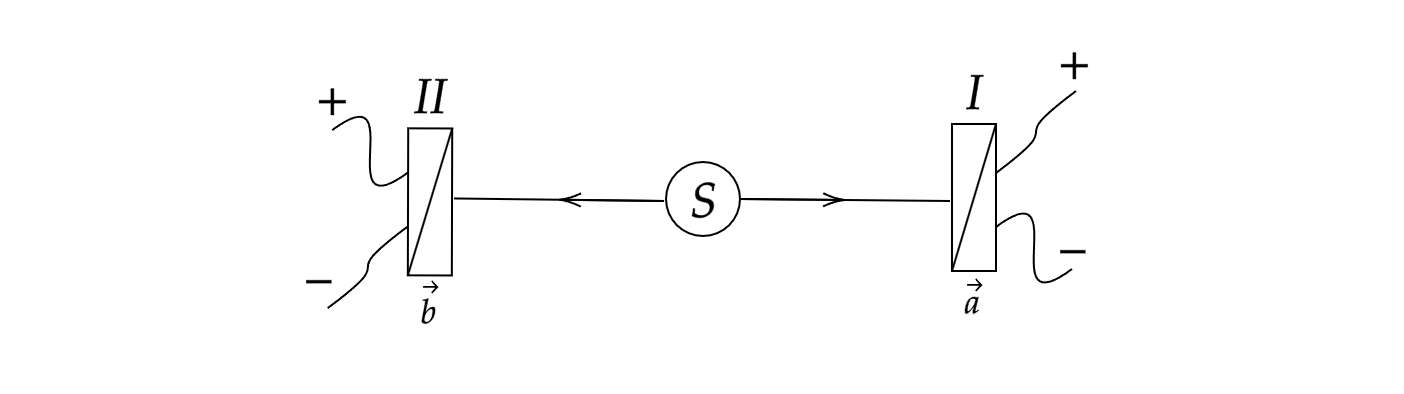
\includegraphics[scale=.25
        ]{Problem_15/image/1.png}
    \end{center}
    \begin{center}
    Hình 1: Thí nghiệm đo phân cực của một cặp photon bị rối
    \end{center}
    \end{figure}
\end{center}
Theo diễn giải cơ học lượng tử của Bohr, xác suất để ngẫu nhiên một photon đi qua $(+)$ một kính phân cực bằng xác suất để nó không đi qua $(-)$: $$P_+(\Vec{a})=P_-(\Vec{a})=\dfrac{1}{2},$$ $$P_+(\Vec{b})=P_-(\Vec{b})=\dfrac{1}{2}.$$
Cũng theo quan điểm này của Bohr, với hệ photon như thí nghiệm của Aspect có xác suất để cả hai photon cùng đi qua $(++)$ hai kính phân cực hoặc cùng không đi qua $(--)$ là bằng nhau và xác suất để một trong hai đi qua kính phân cực I $(+-)$ hoặc II $(-+)$ là bằng nhau: $$P_{++}(\Vec{a},\Vec{b})=P_{--}(\Vec{a},\Vec{b})=\dfrac{1}{2}\cos^2\theta,$$
$$P_{+-}(\Vec{a},\Vec{b})=P_{-+}(\Vec{a},\Vec{b})=\dfrac{1}{2}\sin^2\theta.$$
Trong đó $\theta$ là góc tạo bởi $\Vec{a}$ và $\Vec{b}$.
\begin{enumerate}[label=\textbf{\alph*,}]\itemsep0em
    \item Xét trường hợp đặc biệt khi cả hai kính phân cực có cùng phương phân cực, Xác suất để cả hai photon cùng đi, cùng không đi qua và chỉ một trong hai photon đi qua kính phân cực là bao nhiêu ?
    \item Xét đại lượng $E(\Vec{a},\Vec{b})$ được gọi là \textit{"tương quan giữa hai photon"}. Nếu lý thuyết biến ẩn không tồn tại và diễn giải của Bohr đúng, "tương quan" giữa hai photon được xác định là: $$E(\Vec{a},\Vec{b})=P_{++}(\Vec{a},\Vec{b})+P_{--}(\Vec{a},\Vec{b})-P_{+-}(\Vec{a},\Vec{b})-P_{-+}(\Vec{a},\Vec{b}).$$
Nếu lý thuyết biến ẩn tồn tại và diễn giải của Bohr sai, "tương quan" giữa hai photon được xác định là:
$$E(\Vec{a},\Vec{b})=\displaystyle\int\limits_{-\infty}^{+\infty}A(\Vec{a},\lambda)B(\Vec{b},\lambda)\rho(\lambda)d\lambda.$$ Tính biểu thức "tương quan" giữa hai photon chỉ phụ thuộc vào $\theta$ nếu không tồn tại biến số ẩn.
    \item Bây giờ ta xây dựng tiếp thí nghiệm của Aspect, đó là thêm ở đầu đo I kính phân cực có phương $\Vec{a'}$ và thêm ở đầu đo II kính phân cực có phương $\Vec{b'}$ sao cho phương phân cực của các kính tạo thành các góc như \textbf{(Hình 2)}, lúc này photon đi đến đầu đo I phân cực trên phương $\Vec{a}$ và $\Vec{a'}$, tương tự với đầu đo II là $\Vec{b}$ và $\Vec{b'}$ \textbf{(Hình 2)}.
    \begin{center}
    \begin{figure}[htp]
    \begin{center}
        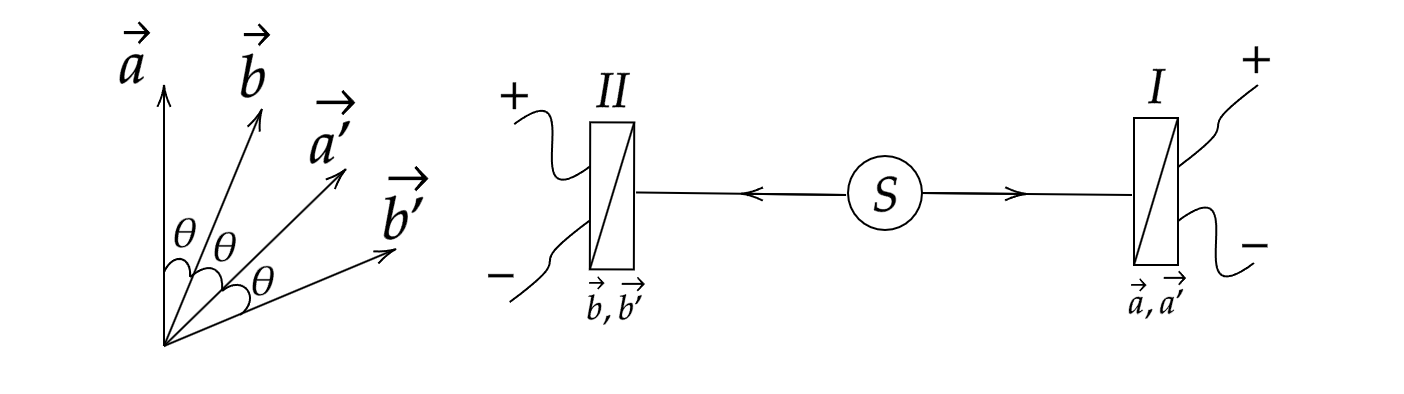
\includegraphics[scale=.25
        ]{Problem_15/image/2.png}
    \end{center}
    \begin{center}
    Hình 2: Thí nghiệm của Alain Aspect
    \end{center}
    \end{figure}
\end{center}
Ta xây dựng biểu thức "tương quan" giữa hai photon dựa trên lý thuyết biến ẩn. Khi tiến hành phép đo hai photon đồng thời với nhau, kết quả phép đo thu được là tổ hợp các trường hợp phân cực có thể xảy ra trên hai đầu đo và bằng tích $AB$. Ta xét đại lượng sau:
$$s(\Vec{a},\Vec{a'},\Vec{b},\Vec{b'},\lambda)=A(\Vec{a},\lambda)B(\Vec{b},\lambda)-A(\Vec{a},\lambda)B(\Vec{b'},\lambda)+A(\Vec{a'},\lambda)B(\Vec{b},\lambda)+A(\Vec{a'},\lambda)B(\Vec{b'},\lambda).$$
Trong đó $A$ và $B$ chỉ có thể nhận các giá trị $-1$ hoặc $+1$.\\
Và giá trị trung bình của đại lượng $s(\Vec{a},\Vec{a'},\Vec{b},\Vec{b'},\lambda)$ được định nghĩa là: $$S(\Vec{a},\Vec{a'},\Vec{b},\Vec{b'})=\displaystyle\int\limits_{-\infty}^{+\infty}s(\Vec{a},\Vec{a'},\Vec{b},\Vec{b'},\lambda)\rho(\lambda)d\lambda.$$
\begin{enumerate}
    \item Đại lượng $s(\Vec{a},\Vec{a'},\Vec{b},\Vec{b'},\lambda)$ chỉ có thể nhận những giá trị nào ?
    \item Giả sử lý thuyết biến ẩn tồn tại và diễn giải cơ học lượng tử của Bohr sai, xác định điều kiện biên của $S(\Vec{a},\Vec{a'},\Vec{b},\Vec{b'})$.
    \item Giả sử lý thuyết biến ẩn không tồn tại và diễn giải cơ học lượng tử của Bohr đúng, xác định điều kiện biên của $S(\Vec{a},\Vec{a'},\Vec{b},\Vec{b'})$.
    \item Đồ thị bên dưới \textbf{(Hình 3)} là kết quả thực nghiệm của Aspect đo đại lượng $S(\Vec{a},\Vec{a'},\Vec{b},\Vec{b'})$ khi thay đổi góc $\theta$. Dựa vào kết quả bạn tìm được ở trên, theo bạn từ kết quả thực nghiệm, lý thuyết biến ẩn đúng hay diễn giải cơ học lượng tử của Bohr đúng? Vậy Einstein hay Bohr đã sai về sự tồn tại của biến số ẩn?
    \begin{center}
    \begin{figure}[htp]
    \begin{center}
        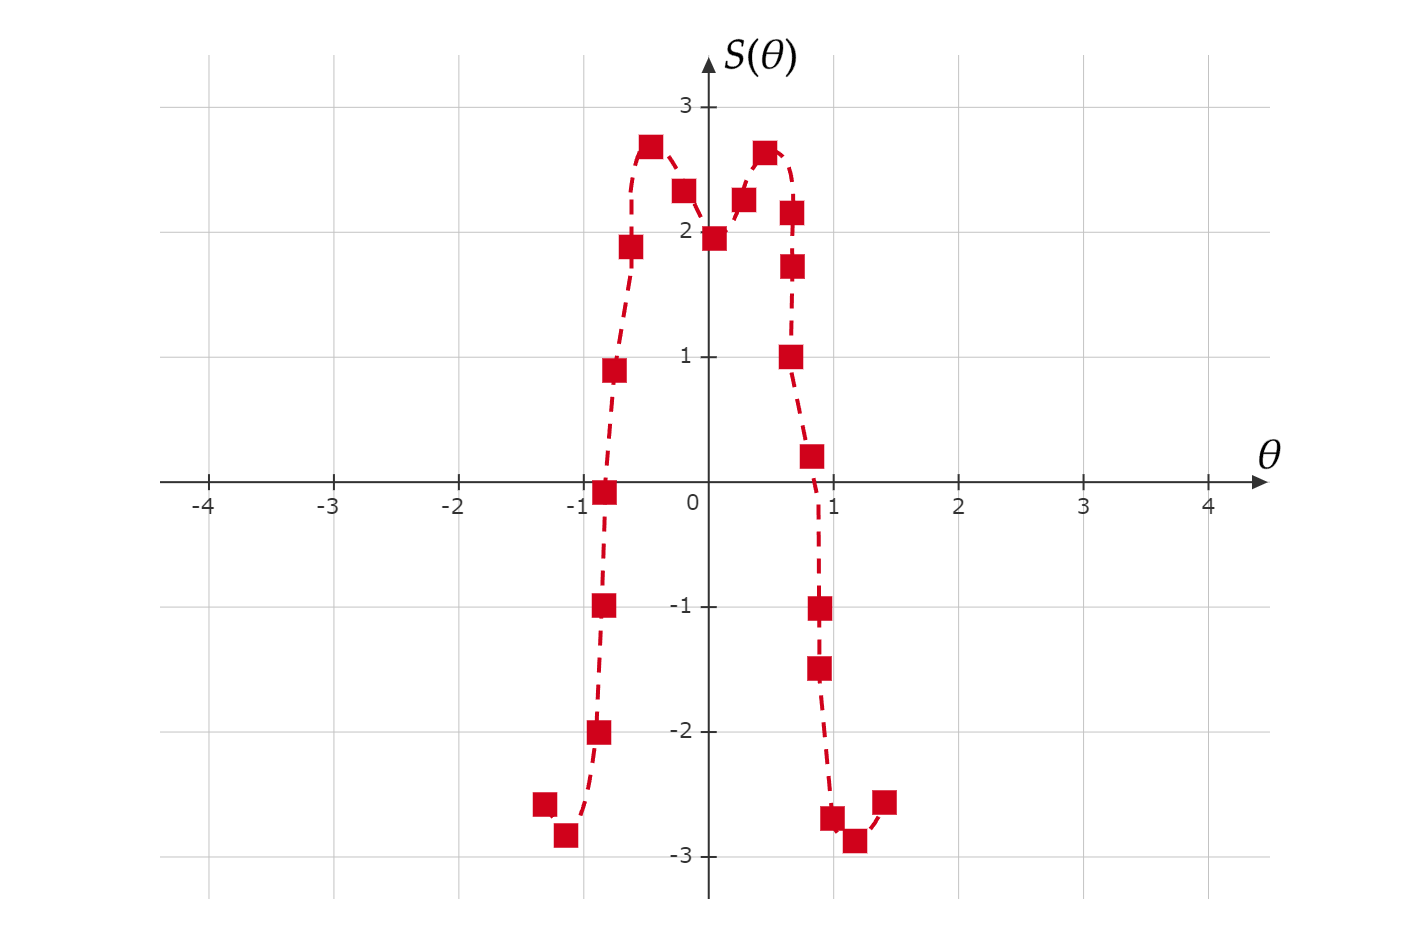
\includegraphics[scale=.22
        ]{Problem_15/image/3.png}
    \end{center}
    \begin{center}
    Hình 3: Kết quả thực nghiệm
    \end{center}
    \end{figure}
\end{center}
\end{enumerate}
\end{enumerate}

\end{enumerate}
\begin{flushright}
    (Biên soạn bởi Nhân viên phòng lab)
\end{flushright}
\setcounter{equation}{0}
\begin{center}
    \normalcolor{\textbf{Bài giải}}
\end{center}
\begin{enumerate}
    \item \textbf{Bất đẳng thức Bell.} \\
    \begin{enumerate}[label=\textbf{\alph*,}]\itemsep0em
        \item Do $A(\Vec{a},\lambda)$ và $B(\Vec{b},\lambda)$ là kết quả đo spin của hạt 1 và hạt 2 lần lượt trên vector đơn vị $\Vec{a}$ và $\Vec{b}$ mà $A$ không ảnh hưởng đến $B$ nên $A(\Vec{a},\lambda)$ và $B(\Vec{b},\lambda)$ chỉ nhận giá trị sau:
\begin{align}
    \label{eq1_Bell}
    A(\Vec{a},\lambda)=\Vec{\sigma}_1\cdot \Vec{a}= \pm 1, \\
    \label{eq2_Bell}
    B(\Vec{b},\lambda)=\Vec{\sigma}_2\cdot \Vec{b}= \pm 1.
\end{align}
    \item \begin{enumerate}
        \item Trong trường hợp $\Vec{a}=\Vec{b}$, hai hạt chắc chắn có spin phản song song nhau, khi đó: 
\begin{align}
    \label{eq3_Bell}
    A(\Vec{a},\lambda)=-B(\Vec{a},\lambda),\\
    \label{eq4_Bell}
    A(\Vec{b},\lambda)=-B(\Vec{b},\lambda).
\end{align}
       \item Thay phương trình (\ref{eq1_Bell}) và phương trình (\ref{eq3_Bell}) vào công thức tính giá trị trung bình trong đề bài, ta được giá trị trung bình của kết quả phép đo $\Vec{\sigma}_1$ đo trên $\Vec{a}$ và $\Vec{\sigma}_2$ đo trên $\Vec{b}$ xảy ra đồng thời:
       \begin{align}
    P(\Vec{a},\Vec{a})&=-\displaystyle\int\limits_{-\infty}^{+\infty}A(\Vec{a},\lambda)A(\Vec{a},\lambda)\rho(\lambda)d\lambda=-\displaystyle\int\limits_{-\infty}^{+\infty}\left[A(\Vec{a},\lambda)\right]^2\rho(\lambda)d\lambda \nonumber \\
    \label{eq5_Bell}
    &=-\displaystyle\int\limits_{-\infty}^{+\infty}\rho(\lambda)d\lambda=-1.
\end{align}
        \item Từ kết quả (\ref{eq4_Bell}), thay vào công thức tính giá trị trung bình $P(\Vec{a},\Vec{b})$, ta được:
\begin{align} \label{eq6_Bell}
    P(\Vec{a},\Vec{b})=-\displaystyle\int\limits_{-\infty}^{+\infty}A(\Vec{a},\lambda)A(\Vec{b},\lambda)\rho(\lambda)d\lambda.
\end{align}
    \end{enumerate}
    \item Tương tự kết quả (\ref{eq6_Bell}), ta tổng quát hoá với trường hợp $\Vec{a}$ và $\Vec{c}$, $\Vec{c}$ có vai trò như $\Vec{b}$ nên ta chỉ cần thay $\Vec{b}$ thành $\Vec{c}$:
\begin{align} \label{eq7_Bell}
    P(\Vec{a},\Vec{c})=-\displaystyle\int\limits_{-\infty}^{+\infty}A(\Vec{a},\lambda)A(\Vec{c},\lambda)\rho(\lambda)d\lambda.
\end{align}
    \item \begin{enumerate}
        \item Ta tính hiệu $P(\Vec{a},\Vec{b})-P(\Vec{a},\Vec{c})$ từ phương trình (\ref{eq6_Bell}) và phương trình (\ref{eq7_Bell}):
\begin{align}
    P(\Vec{a},\Vec{b})-P(\Vec{a},\Vec{c})&=-\displaystyle\int\limits_{-\infty}^{+\infty}\left[A(\Vec{a},\lambda)A(\Vec{b},\lambda)-A(\Vec{a},\lambda)A(\Vec{c},\lambda)\right]\rho(\lambda)d\lambda\nonumber \\
    \label{eq8_Bell}
    &=-\displaystyle\int\limits_{-\infty}^{+\infty}\left[1-\dfrac{A(\Vec{c},\lambda)}{A(\Vec{b},\lambda)}\right]A(\Vec{a},\lambda)A(\Vec{b},\lambda)\rho(\lambda)d\lambda.
\end{align}
Vì ta đang cần xuất hiện thành phần $A(\Vec{b},\lambda)A(\Vec{c},\lambda)$ để tạo ra thành phần $P(\Vec{b},\Vec{c})$ nên ta nhân vào trước $A(\Vec{c},\lambda)$ số hạng $\left[A(\Vec{b},\lambda)\right]^2$. Theo kết quả (\ref{eq2_Bell}): $\left[A(\Vec{b},\lambda)\right]^2=1$.
\begin{align}
    P(\Vec{a},\Vec{b})-P(\Vec{a},\Vec{c})&=-\displaystyle\int\limits_{-\infty}^{+\infty}\left[1-\left[A(\Vec{b},\lambda)\right]^2\dfrac{A(\Vec{c},\lambda)}{A(\Vec{b},\lambda)}\right]A(\Vec{a},\lambda)A(\Vec{b},\lambda)\rho(\lambda)d\lambda \nonumber \\
    \label{eq9_Bell}
    &=-\displaystyle\int\limits_{-\infty}^{+\infty}A(\Vec{a},\lambda)A(\Vec{b},\lambda)\left[1-A(\Vec{b},\lambda)A(\Vec{c},\lambda)\right]\rho(\lambda)d\lambda.
\end{align}
Ta nhận xét từ phương trình (\ref{eq9_Bell}): Do các giá trị $A$ chỉ có thể nhận các giá trị $+1$ và $-1$ nên ta có:
\begin{align}
    \label{eq10_Bell}
    -1 \leq A(\Vec{a},\lambda)A(\Vec{b},\lambda) \leq + 1, \\
    \label{eq11_Bell}
    -1 \leq A(\Vec{b},\lambda)A(\Vec{c},\lambda) \leq + 1.
\end{align}
Từ kết quả (\ref{eq11_Bell}), ta nhận thấy: $\left[1-A(\Vec{b},\lambda)A(\Vec{c},\lambda)\right]\rho(\lambda) \geq 0$. \\
\begin{enumerate}
\item Xét trường hợp 1: $0 \leq A(\Vec{a},\lambda)A(\Vec{b},\lambda) \leq + 1$. Rõ ràng ta thấy được:
\begin{align}
    \label{eq12_Bell}
    \hspace{-2cm} 0\geq -\displaystyle\int\limits_{-\infty}^{+\infty}A(\Vec{a},\lambda)A(\Vec{b},\lambda)&\left[ 1-A(\Vec{b},\lambda)A(\Vec{c},\lambda)\right]\rho(\lambda)d\lambda \geq -\displaystyle\int\limits_{-\infty}^{+\infty}\left[1-A(\Vec{b},\lambda)A(\Vec{c},\lambda)\right]\rho(\lambda)d\lambda, \\
    \label{eq13_Bell}
    0& \geq P(\Vec{a},\Vec{b})-P(\Vec{a},\Vec{c}) \geq - 1 - P(\Vec{b},\Vec{c}).
\end{align}
\item Xét trường hợp 2: $-1 \leq A(\Vec{a},\lambda)A(\Vec{b},\lambda) \leq 0$. Rõ ràng ta thấy được:
\begin{align}
    \label{eq14_Bell}
    \hspace{-2cm} 0\leq -\displaystyle\int\limits_{-\infty}^{+\infty}A(\Vec{a},\lambda)A(\Vec{b},\lambda)&\left[ 1-A(\Vec{b},\lambda)A(\Vec{c},\lambda)\right]\rho(\lambda)d\lambda \leq -\displaystyle\int\limits_{-\infty}^{+\infty}\left[1-A(\Vec{b},\lambda)A(\Vec{c},\lambda)\right]\rho(\lambda)d\lambda, \\
    \label{eq15_Bell}
    0& \leq P(\Vec{a},\Vec{b})-P(\Vec{a},\Vec{c}) \leq  1 + P(\Vec{b},\Vec{c}).
\end{align}
\end{enumerate}
Như vậy điều kiện liên hệ giữa $P(\Vec{a},\Vec{b})$, $P(\Vec{a},\Vec{c})$ và $P(\Vec{b},\Vec{c})$ từ bất đẳng thức (\ref{eq13_Bell}) và (\ref{eq15_Bell}) là:
\begin{align} \label{eq16_Bell}
    \begin{cases}
    0\leq \ P(\Vec{a},\Vec{c})-P(\Vec{a},\Vec{b})&\leq  1 + P(\Vec{b},\Vec{c}),\\
    0\leq \ P(\Vec{a},\Vec{b})-P(\Vec{a},\Vec{c})&\leq  1 + P(\Vec{b},\Vec{c}).
    \end{cases}
\end{align}
Bất đẳng thức (\ref{eq16_Bell}) có thể viết lại thành:
\begin{align} \label{eq17_Bell}
    \big|P(\Vec{a},\Vec{b})-P(\Vec{a},\Vec{c})\big|&\leq  1 + P(\Vec{b},\Vec{c}).
\end{align}
      \item Thay số theo đề bài:
\begin{align}
    \label{eq18_Bell}
    P(\Vec{a},\Vec{b})&=-\Vec{a}\cdot \Vec{b}=0,\\
    \label{eq19_Bell}
    P(\Vec{a},\Vec{c})&=-\Vec{a}\cdot \Vec{c}=-\dfrac{1}{\sqrt{2}},\\
    \label{eq20_Bell}
    P(\Vec{b},\Vec{c})&=-\Vec{b}\cdot \Vec{c}=-\dfrac{1}{\sqrt{2}}.
\end{align}
Như vậy, từ (\ref{eq17_Bell}), (\ref{eq18_Bell}), (\ref{eq19_Bell}) và (\ref{eq20_Bell}), rõ ràng điều kiện (\ref{eq17_Bell}) bị vi phạm vì: 
$$\left|0+\dfrac{1}{\sqrt{2}}\right| \leq 1-\dfrac{1}{\sqrt{2}}.$$
Kết quả này là vô lý và trường hợp cụ thể này không tồn tại. Vì ta đã xây dựng bài toán và điều kiện (\ref{eq17_Bell}) theo lý thuyết biến ẩn nên trường hợp bị vi phạm đã chỉ ra không tồn tại lý thuyết biến ẩn và cơ học lượng tử theo quan điểm của Bohr đúng.
    \end{enumerate}
    \end{enumerate}
\textit{Bất đẳng thức (\ref{eq17_Bell}) chính xác là bất đẳng thức Bell nổi tiếng, công trình này khi ra đời đã giúp loại bỏ lý thuyết biến số ẩn khỏi cơ học lượng tử và kết luận rằng việc thực hiện phép đo ở một vị trí trong không gian này có thể ảnh hưởng tức thì đến phép đo ở vị trí khác trong không gian kia. Sự ảnh hưởng này là tức thời bất kể khoảng cách, Bell đã thừa nhận sự tồn tại của "tác dụng ma quái theo khoảng cách". Tuy nhiên, các nhà khoa học dù phần lớn tin vào trường phái Copenhagen của Bohr nhưng vẫn có những người vẫn chọn tin vào Einstein, đều đó mới dẫn đến các thí nghiệm kiểm chứng bất đẳng thức Bell sau này của Clauser, Aspect và Zeilinger.}

    \item \textbf{Kiểm chứng bất đẳng thức Bell bằng thực nghiệm và giải Nobel 2022.} \\
    \begin{enumerate}[label=\textbf{\alph*,}]\itemsep0em
        \item Khi phương phân cực của hai kính giống nhau $\Vec{a}=\Vec{b}$,     xác suất để hai photon cùng đi qua bằng xác suất để cùng không đi qua và không tồn tại trường hợp chỉ một trong hai đi qua, do:
\begin{align}
    \label{eq21_Bell}
    P_{++}(\Vec{a},\Vec{a})=P_{--}(\Vec{a},\Vec{a})=\dfrac{1}{2},\\
    \label{eq22_Bell}
    P_{+-}(\Vec{a},\Vec{a})=P_{-+}(\Vec{a},\Vec{a})=0.
\end{align}
    \item "Tương quan" giữa hai photon theo diễn giải của Bohr:
\begin{align}
    E(\Vec{a},\Vec{b})&=P_{++}(\Vec{a},\Vec{b})+P_{--}(\Vec{a},\Vec{b})-P_{+-}(\Vec{a},\Vec{b})-P_{-+}(\Vec{a},\Vec{b})\nonumber \\
    \label{eq23_Bell}
    &=\cos^2\theta - \sin^2\theta = \cos 2 \theta.
\end{align} 
     \item \begin{enumerate}
         \item Ta biến đổi đại lượng $s(\Vec{a},\Vec{a'},\Vec{b},\Vec{b'},\lambda)$:
\begin{align}
    s(\Vec{a},\Vec{a'},\Vec{b},\Vec{b'},\lambda)&=A(\Vec{a},\lambda)B(\Vec{b},\lambda)-A(\Vec{a},\lambda)B(\Vec{b'},\lambda)+A(\Vec{a'},\lambda)B(\Vec{b},\lambda)+A(\Vec{a'},\lambda)B(\Vec{b'},\lambda) \nonumber \\ 
    \label{eq24_Bell}
    &=A(\Vec{a},\lambda)\left[B(\Vec{b},\lambda)-B(\Vec{b'},\lambda)\right]+A(\Vec{a'},\lambda)\left[B(\Vec{b},\lambda)+B(\Vec{b'},\lambda)\right].
\end{align}
Từ đề bài, do $A$ và $B$ chỉ có thể nhận giá trị $-1$ hoặc $+1$ nên $s(\Vec{a},\Vec{a'},\Vec{b},\Vec{b'},\lambda)$ chỉ có thể nhận giá trị $+2$ hoặc $-2$. 
\item Giả sử lý thuyết biến ẩn tồn tại và diễn giải của Bohr sai. Giá trị trung bình $S(\Vec{a},\Vec{a'},\Vec{b},\Vec{b'})$ của $s(\Vec{a},\Vec{a'},\Vec{b},\Vec{b'},\lambda)$ là phải nằm trong khoảng $-2$ đến $+2$ do $s(\Vec{a},\Vec{a'},\Vec{b},\Vec{b'},\lambda)$ chỉ có thể nhận giá trị $+2$ hoặc $-2$ (giả sử ta đo ra $m$ giá trị $+2$, $n$ giá trị $-2$, trung bình sẽ là $\dfrac{2(m-n)}{m+n}$ và nằm trong khoảng $-2$ đến $+2$)
\begin{align} \label{eq25_Bell}
    -2\leq S(\Vec{a},\Vec{a'},\Vec{b},\Vec{b'}) \leq 2.
\end{align}
Ngoài ra, khi ta sử dụng định nghĩa giá trị trung bình trong đề bài, ta thu được như sau:
\begin{align}
    S(\Vec{a},\Vec{a'},\Vec{b},\Vec{b'})&=\displaystyle\int\limits_{-\infty}^{+\infty}s(\Vec{a},\Vec{a'},\Vec{b},\Vec{b'},\lambda)\rho(\lambda)d\lambda \nonumber \\
    \label{eq26_Bell}
    &=E(\Vec{a},\Vec{b})-E(\Vec{a},\Vec{b'})+E(\Vec{a'},\Vec{b})+E(\Vec{a'},\Vec{b'}).
\end{align}
Đây chính là biểu diễn của đại lượng $S(\Vec{a},\Vec{a'},\Vec{b},\Vec{b'})$.
\item Giả sử lý thuyết biến ẩn không tồn tại và diễn giải của Bohr đúng. Giá trị trung bình $S(\Vec{a},\Vec{a'},\Vec{b},\Vec{b'})$ so với xây dựng từ lý thuyết biến ẩn đều phải mô tả cùng một đại lượng vật lý nào đó. Từ phương trình (\ref{eq23_Bell}) và phương trình (\ref{eq26_Bell}):
\begin{align}
    S(\Vec{a},\Vec{a'},\Vec{b},\Vec{b'})&=E(\Vec{a},\Vec{b})-E(\Vec{a},\Vec{b'})+E(\Vec{a'},\Vec{b})+E(\Vec{a'},\Vec{b'}) \nonumber \\
    &= \cos 2\theta - \cos 6\theta + \cos 2\theta + \cos 2\theta \nonumber \\
    \label{eq27_Bell}
    &= 3\cos 2\theta - \cos 6\theta.
\end{align}
Đại lượng $S(\Vec{a},\Vec{a'},\Vec{b},\Vec{b'})$ đạt cực trị khi $\dfrac{dS}{d\theta}=0$:
\begin{align}
    &\ \ \ \ \ \ \ \ \ \ \ \ \ \ \ \ \ \ \ \ \ \ \ \ \ \ \ \ \ \ \ \ \ \    \dfrac{dS}{d\theta}=0 \nonumber \\
    &\ \ \ \ \ \ \ \ \ \ \ \ \ \ \ \ \ \ \ \ \ \ \ \ \ \ \sin 6\theta - \sin 2\theta =0 \nonumber \\
    &\ \ \  2\sin 2\theta \cos^2 2\theta + \sin 2\theta \left(\cos^2 2\theta - \sin^2 2\theta\right)-\sin 2\theta = 0\nonumber \\
    &\sin 2\theta \left(2 \cos^2 2\theta + \cos^2 2\theta - \sin^2 2\theta -\cos^2 2\theta-\sin^2 2\theta\right)=0\nonumber \\
    \label{eq28_Bell}
    &\ \ \ \ \ \ \ \ \ \ \ \ \ \ \ \ \ \ \ \ \ \ \ \ \ \ \  \sin 2\theta \cos 4\theta =0.
\end{align}
Từ phương trình (\ref{eq28_Bell}), suy ra cực trị của $S(\Vec{a},\Vec{a'},\Vec{b},\Vec{b'})$ \Big(do $S(\theta)$ là hàm lượng giác có công thức như (\ref{eq27_Bell}) nên để tìm cực trị của $S$ ta chỉ cần xét $-\dfrac{\pi}{2}\leq \theta \leq +\dfrac{\pi}{2}$\Big):
\begin{align} \label{eq29_Bell}
    \begin{cases}
        \theta_{\text{extr}} =0,\pm \dfrac{ \pi}{2}\ \ \ \ \ \ \ \ \ \ \ \ S_{\text{extr}} = \pm 2, \\ \\
        \theta_{\text{extr}} = \pm\dfrac{3\pi}{8}\ \ \ \ \ \ \ \ \ \ \ \ \   S_{\text{extr}} =  -2\sqrt{2}, \\ \\
        \theta_{\text{extr}} = \pm\dfrac{\pi}{8}\ \ \ \ \ \ \ \ \ \ \ \ \ \ \  S_{\text{extr}} = +2\sqrt{2}.
    \end{cases}
\end{align}
Như vậy, theo quan điểm cơ học lượng tử của Bohr, điều kiện biên của $S(\Vec{a},\Vec{a'},\Vec{b},\Vec{b'})$:
\begin{align} \label{eq30_Bell}
    -2\sqrt{2}\leq S(\Vec{a},\Vec{a'},\Vec{b},\Vec{b'}) \leq +2\sqrt{2}.
\end{align}
\item Từ bất đẳng thức (\ref{eq25_Bell}) và bất đẳng thức (\ref{eq30_Bell}), nếu tồn tại kết quả thực nghiệm nằm trong khoảng $[-2\sqrt{2},-2]$ và $[2,2\sqrt{2}]$ thì có thể kết luận quan điểm cơ học lượng tử của Bohr đúng.\\
\end{enumerate}
\begin{itemize}
    \item Diễn giải suy sập hàm sóng do phép đo của Bohr: $$-2\sqrt{2}\leq S(\Vec{a},\Vec{a'},\Vec{b},\Vec{b'}) \leq +2\sqrt{2}.$$
    \item Lý thuyết biến số ẩn của Einstein:   $$-2\leq S(\Vec{a},\Vec{a'},\Vec{b},\Vec{b'}) \leq +2.$$
\end{itemize}
\begin{center}
    \begin{figure}[htp]
    \begin{center}
        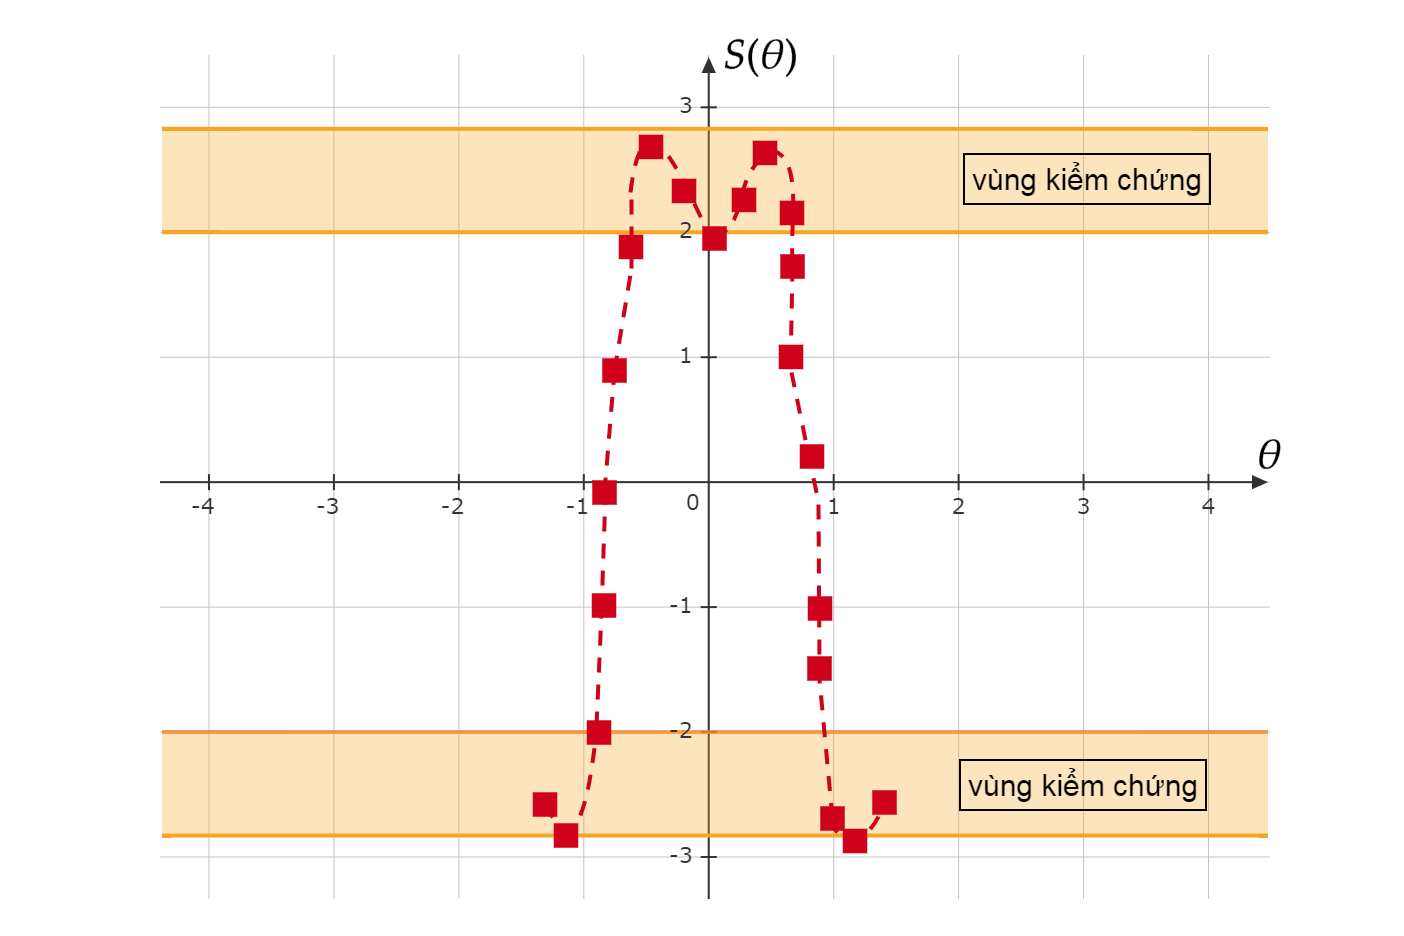
\includegraphics[scale=.22
        ]{Problem_15/image/4.png}
    \end{center}
    \begin{center}
        Hình 4: Tồn tại các kết quả thực nghiệm nằm trong khoản $[-2\sqrt{2},-2]$ và $[2,2\sqrt{2}]$.
    \end{center}
    \end{figure}
\end{center}
Từ đồ thị \textbf{(Hình 4)} ta thấy kết quả thực nghiệm đã chỉ ra diễn giải của Bohr đúng và lý thuyết biến ẩn không tồn tại. Vậy Einstein đã sai và Bohr đã đúng về sự tồn tại của biến số ẩn!
     \end{enumerate}
     \textit{Bất đẳng thức (\ref{eq25_Bell}) là bất đẳng thức CHSH mang chữ cái đầu của 4 tác giả Clauser, Horne, Shimony và Holt. Đây là cách thể hiện khác của bất đẳng thức Bell, được đề xuất bằng cách thay việc đo spin của các hạt thực bằng việc đo hướng phân cực của photon. Kết quả thực nghiệm của các nhà vật lý đã chỉ ra không có biến số ẩn, các hạt vi mô không có định xứ, sự rối lượng tử giữa các hạt là tức thời bất kể khoảng cách bao xa, "tác dụng ma quái theo khoảng cách" không chỉ có thật mà còn là bản chất của các hạt vi mô. Ngoài ra "tác dụng ma quái theo khoảng cách" cũng không còn ma quái khi các nhà khoa học đã chứng minh nó không vi phạm thuyết tương đối vì không có thông tin nào được truyền đi giữa các hạt.}
    \end{enumerate}

\textbf{Biểu điểm}
\begin{center}
\begin{tabular}{|>{\centering\arraybackslash}m{1cm}|>{\raggedright\arraybackslash}m{14cm}| >{\centering\arraybackslash}m{1cm}|}
    \hline
    \textbf{Phần} & \textbf{Nội dung} & \textbf{Điểm} \\
    \hline
    \textbf{1a} & Viết được kết quả (\ref{eq1_Bell}) và (\ref{eq2_Bell}) & $0.50$ \\
    \hline 
    \textbf{1b.i} & Viết được kết quả (\ref{eq3_Bell}) và (\ref{eq4_Bell}) & $0.50$ \\
    \hline 
    \textbf{1b.ii} & Viết được kết quả (\ref{eq5_Bell}) & $0.50$ \\
    \hline 
    \textbf{1b.iii} & Viết được kết quả (\ref{eq6_Bell}) & $0.50$ \\
    \hline 
    \textbf{1c} & Viết được kết quả (\ref{eq7_Bell}) & $0.50$ \\
    \hline 
    \textbf{1d.i} & Viết biểu thức hiệu $P(\Vec{a},\Vec{b})-P(\Vec{a},\Vec{c})$ (\ref{eq9_Bell}) & $2.00$ \\
    \cline{2-3}
    &  Viết được bất đẳng thức (\ref{eq10_Bell}) và (\ref{eq11_Bell}) & $0.50$ \\
    \cline{2-3}
    &  Viết được bất đẳng thức (\ref{eq16_Bell}) hoặc (\ref{eq17_Bell}) & $2.00$ \\
    \hline
    \textbf{1d.ii} & Chỉ ra bất đẳng thức (\ref{eq17_Bell}) bị vi phạm & $0.50$ \\
    \cline{2-3}
    &  Kết luận về sự tồn tại của biến số ẩn & $0.50$ \\
    \hline
    \textbf{2a} & Viết được kết quả (\ref{eq21_Bell}) và (\ref{eq22_Bell}) & $0.50$ \\
    \hline
    \textbf{2b} & Viết biểu thức "tương quan" giữa hai photon theo diễn giải của Bohr (\ref{eq23_Bell}) & $0.50$ \\
    \hline
    \textbf{2c.i} & Viết được biểu thức (\ref{eq24_Bell}) & $0.50$ \\
    \hline
    \textbf{2c.ii} & Chỉ ra đại lượng $s(\Vec{a},\Vec{a'},\Vec{b},\Vec{b'},\lambda)$ chỉ có thể nhận các giá trị $\pm 2$ & $0.50$ \\
    \cline{2-3}
    & Viết được bất đẳng thức (\ref{eq25_Bell}) & $1.50$ \\
    \cline{2-3}
    & Viết được biểu thức (\ref{eq26_Bell}) & $0.50$ \\
    \hline
    \textbf{2c.iii} & Viết được biểu thức (\ref{eq27_Bell}) & $0.50$ \\
    \cline{2-3}
    & Tìm được các cực trị của đại lượng $S$ (\ref{eq29_Bell}) & $1.50$ \\
    \cline{2-3}
    & Viết được bất đẳng thức (\ref{eq30_Bell}) & $1.50$ \\
    \hline
    \textbf{2c.iv} & Lập luận và so sánh với kết quả trong đồ thị. Kết luận. & $0.50$ \\
    \hline
\end{tabular}
\end{center}

%% Reference %%
\bibliographystyle{plain}
\begin{thebibliography}{}
\bibitem{bell1964} John S. Bell (1964), \textit{On the Einstein Podolsky Rosen paradox}, Physics Physique Fizika 1, 195 – Published 1 November 1964.        
\bibitem{clauser1970} John F. Clauser, Michael A. Horne, Abner Shimony, and Richard A. Holt (1970), \textit{Proposed Experiment to Test Local Hidden-Variable Theories}, Physical Review Letters, Volume 23, Issue 15, Pages 880-884.
\bibitem{aspect1976} Alain Aspect (1976), \textit{Proposed experiment to test the nonseparability of quantum mechanics}, Physical Review D, Volume 14, Issue 8, Pages 1944-1951.
\end{thebibliography}



\newpage
{\normalcolor \textbf{CÂU 16 (8 điểm)}}\vspace{1.5mm}

\setcounter{equation}{0}
%Bài toán đề xuất bởi NVPL

\textbf{Pha trộn và dao động neutrino}

\textit{Neutrino} là một trong các hạt cơ bản của vũ trụ mà đã được con người phát hiện ra. Các nghiên cứu về neutrino là một trong những nghiên cứu tiền tuyến của vật lý hạt cơ bản do các hạt neutrino chuyển động rất nhanh (tiệm cận vận tốc ánh sáng) và chỉ tham gia vào tương tác yếu và tương tác hấp dẫn nên rất khó để "bắt" được dấu vết của các hạt neutrino. Theo \textit{Mô hình Chuẩn (Standard Model)}, các hạt neutrino được giả định là không có khối lượng; tuy nhiên số liệu từ thí nghiệm phân rã hạt $\beta$ của tritium $^3\text{H}$ tương thích với khả năng các hạt neutrino có khối lượng khác không. Trong bài tập này ta sẽ tìm hiểu về hiện tượng dao động neutrino dựa trên các cách tiếp cận phổ thông và trực quan hơn bên cạnh cách tiếp cận chính thống là lý thuyết trường lượng tử để đánh giá và tìm hiểu cách mà các nhà vật lý đã kiểm chứng được các hạt neutrino có khối lượng.

\begin{enumerate}
    \item \textbf{Hiện tượng phách}\\
    Theo cơ học lượng tử, hàm sóng liên kết của hai trạng thái có tần số gần giống nhau sẽ xảy ra hiện tượng phách, tương tự như khi chồng chập hai sóng âm có tần số gần giống nhau trong vật lý cổ điển. Giả sử ta có hai hàm sóng $A_1$ và $A_2$ có tần số góc khác nhau lần lượt là $\omega_1$ và $\omega_2$:
    \begin{align*}
        A_1(t)&=Ae^{-i\omega_1 t},\\
        A_2(t)&=-Ae^{-i\omega_2 t}.
    \end{align*}
    \begin{enumerate}
    \item Xác định biểu thức môđun phức bình phương của hàm sóng liên kết hai trạng thái tại thời điểm $t$ bất kỳ.
    \item Giả sử $\omega_1$ và $\omega_2$ là tần số góc ứng với hai trạng thái của hạt nào đó chuyển động với vận tốc tiệm cận vận tốc ánh sáng có năng lượng lần lượt là $E_1$ và $E_2$. Dựa trên quan điểm của de Broglie về lưỡng tính sóng-hạt của vật chất. Biểu diễn biểu thức môđun phức bình phương của hàm sóng liên kết hai trạng thái tại thời điểm $t$ bất kỳ theo năng lượng $E_1$, $E_2$ và các hằng số liên quan.
    \end{enumerate}
    \item \textbf{Độ dài dao động của neutrino}\\
    Các nhà vật lý đã giả thiết rằng, nếu hạt neutrino $a$ nào đó thực sự có khối lượng, ứng với mỗi trạng thái năng lượng $E_n$ của nó thì hạt sẽ có khối lượng $m_n$ tương ứng. Nếu xảy ra sự liên kết giữa hai hàm sóng mô tả hai trạng thái có khối lượng khác nhau của hạt neutrino thì sẽ xảy ra hiện tượng phách, sự liên kết này được gọi là \textit{pha trộn neutrino (neutrino mixing)}. Trong quá trình pha trộn neutrino, qua thời gian, hạt neutrino $a$ liên tục biến thành hạt neutrino $b$ và ngược lại, ứng với pha của hàm sóng liên kết, quá trình này được gọi là \textit{dao động neutrino (neutrino oscillations)}. Giả sử ban đầu ở lò phản ứng hạt nhân chỉ phát ra chùm hạt neutrino $a$ theo phương $x$, tỉ lệ giữa số hạt neutrino $b$ biến đổi từ neutrino $a$ ở thời điểm $t$ so với số hạt neutrino $a$ ở thời điểm ban đầu được tính theo biểu thức:
    $$P_{\alpha \rightarrow \beta}=\sin^2(2\theta)\sin^2\left(\dfrac{E_m-E_n}{2\hbar}t\right)=\sin^2(2\theta)\sin^2\left(\dfrac{x}{L_0}\right).$$
    Trong đó $\theta$ được gọi là góc pha trộn, $L_0$ được gọi là độ dài dao động của neutrino.\\
    Xác định biểu thức độ dài dao động của neutrino theo $E_m$, $E_n$ và các hằng số liên quan.

\item \textbf{Thí nghiệm KamLAND}\\
Thí nghiệm KamLAND (The Kamioka Liquid-scintillator Anti-Neutrino Detector) nghiên cứu về dao động của phản hạt neutrino electron $\overline{\nu_e}$ sau khi bay ra từ lò phản ứng hạt nhân với vận tốc tiệm cận vận tốc ánh sáng ở khoảng cách $x \approx 170 \ \si{km}$ so với lò phản ứng. Tại đó, số hạt $\overline{\nu_e}$ chỉ còn $20\%$ so với ban đầu. Giả thiết các hạt $\overline{\nu_e}$ chỉ có các trạng thái $E_m$ và $E_n$. Năng lượng trung bình của các hạt $\overline{\nu_e}$ là $E \approx E_m \approx E_n \approx 4 \ \si{MeV}$ và $E_m \gg m_m c^2$, $E_n \gg m_n c^2$. Cho biết góc pha trộn $\theta = 45^o$. \\
Tính hiệu số bình phương khối lượng $\Delta m^2 = m_m^2 - m_n^2$ theo đơn vị $\si{(eV)^2/c^4}$.
\end{enumerate}

\begin{flushright}
    (Biên soạn bởi Nhân viên phòng lab)
\end{flushright}
\setcounter{equation}{0}
\begin{center}
    \normalcolor{\textbf{Bài giải}}
\end{center}
\begin{enumerate} 
    \item  \textbf{Hiện tượng phách}\\
    \begin{enumerate}
        \item Hàm sóng liên kết hai trạng thái:
        \begin{equation} \label{eq1_neutrino_oscillation}
            A_{\text{tot}}(t)=A_1(t)+A_2(t)=A\left(e^{-i\omega_1 t}-e^{-i\omega_2 t}\right).
        \end{equation}
        Môđun phức bình phương của hàm sóng liên kết:
        \begin{equation} \label{eq2_neutrino_oscillation}
        \begin{split}
            |A_{\text{tot}}(t)|^2&=A^2\left(e^{-i\omega_1 t}-e^{-i\omega_2 t}\right)\left(e^{i\omega_1 t}-e^{i\omega_2 t}\right) \\ 
            &= A^2\left(2-e^{i(\omega_1-\omega_2) t}-e^{-i(\omega_1-\omega_2) t}\right) \\ 
            &=A^2\left[2-2\cos\left((\omega_1-\omega_2) t\right)\right] \\ 
            &=4A^2 \sin^2 \left(\dfrac{\omega_1-\omega_2}{2}t\right).
        \end{split}   
        \end{equation}
    \item Dựa trên lý thuyết về sóng vật chất của de Broglie, liên hệ giữa tần số góc và năng lượng của hạt:
    \begin{equation} \label{eq3_neutrino_oscillation}
        E=\hbar \omega .
    \end{equation}
    Môđun phức bình phương của hàm sóng từ phương trình (2) viết lại thành:
    \begin{equation} \label{eq4_neutrino_oscillation}
        |A_{\text{tot}}(t)|^2 =4A^2 \sin^2 \left(\dfrac{E_1-E_2}{2\hbar}t\right).
    \end{equation}
    \end{enumerate}
    \item \textbf{Độ dài dao động của neutrino}\\
Tại thời điểm $t$ chùm hạt neutrino bay đến vị trí $x$:
\begin{equation} \label{eq5_neutrino_oscillation}
    x=ct.
\end{equation}
Từ đề bài ta suy ra:
\begin{equation} \label{eq6_neutrino_oscillation}
    \dfrac{E_m-E_n}{2\hbar}t=\dfrac{x}{L_0}=\dfrac{ct}{L_0}.
\end{equation}
Độ dài dao động của neutrino:
\begin{equation} \label{eq7_neutrino_oscillation}
    L_0=\dfrac{2\hbar c}{E_m-E_n}.
\end{equation}
\item \textbf{Thí nghiệm KamLAND}\\
Tại thời điểm $t$, hạt $\overline{\nu_e}$ bay đến vị trí $x$, do số hạt $\overline{\nu_e}$ còn $20\%$ so với ban đầu nên tỉ lệ hạt $\overline{\nu_e}$ đã biến đổi thành hạt khác (giả sử hạt $\nu_\alpha$ nào đó) so với ban đầu là:
\begin{equation} \label{eq8_neutrino_oscillation}
    P_{\overline{\nu_e} \rightarrow \nu_\alpha}=1-0.2=0.8.
\end{equation}
Mặt khác, từ biểu thức tỉ lệ số hạt bị biến đổi ở đề bài, ta suy ra:
\begin{equation} \label{eq9_neutrino_oscillation}
    P_{\overline{\nu_e} \rightarrow \nu_\alpha}=\sin^2(2\theta)\sin^2\left(\dfrac{x}{L_0}\right).
\end{equation}
Từ phương trình (\ref{eq7_neutrino_oscillation}), phương trình (\ref{eq9_neutrino_oscillation}) có thể viết lại thành:
\begin{equation} \label{eq10_neutrino_oscillation}
    \dfrac{x}{2\hbar c}(E_m-E_n)=\arcsin \left(\dfrac{\sqrt{P_{\overline{\nu_e} \rightarrow \nu_\alpha}}}{\sin (2\theta)}\right).
\end{equation}
Ta sẽ biến đổi lại phương trình (\ref{eq10_neutrino_oscillation}) để xuất hiện hiệu số bình phương khối lượng $\Delta m^2$. Năng lượng của từng trạng thái $E_m$ và $E_n$ biểu diễn theo thuyết tương đối hẹp như sau:
\begin{align}
    \label{eq11_neutrino_oscillation}
    E_m&=\sqrt{p^2c^2+m_m^2c^4} \approx pc, \\
    \label{eq12_neutrino_oscillation}
    E_n&=\sqrt{p^2c^2+m_n^2c^4} \approx pc. 
\end{align}
Hiệu $E_m-E_n$ gần đúng đến bậc nhất của khối lượng bình phương:
\begin{align}
    E_m-E_n&=\sqrt{p^2c^2+m_m^2c^4}-\sqrt{p^2c^2+m_n^2c^4} \approx pc\left(1+\dfrac{m_m^2c^4}{2p^2c^2}-1-\dfrac{m_n^2c^4}{2p^2c^2}\right) \nonumber \\
    \label{eq13_neutrino_oscillation}
    &= \dfrac{(m_m^2-m_n^2)c^4}{2pc} = \dfrac{\Delta m^2 c^4}{2E}.
\end{align}
    Từ phương trình (\ref{eq10_neutrino_oscillation}) và phương trình (\ref{eq13_neutrino_oscillation}), ta suy ra biểu thức của hiệu số bình phương khối lượng theo các tham số đã biết:
    \begin{equation} \label{eq14_neutrino_oscillation}
        \dfrac{x\Delta m^2 c^4}{4\hbar c E} =\arcsin \left(\dfrac{\sqrt{P_{\overline{\nu_e} \rightarrow \nu_\alpha}}}{\sin (2\theta)}\right) \Rightarrow 
        \Delta m^2 = \dfrac{4\hbar E}{c^3x}\arcsin \left(\dfrac{\sqrt{P_{\overline{\nu_e} \rightarrow \nu_\alpha}}}{\sin (2\theta)}\right).
    \end{equation}
    Thay số từ đề bài: $\Delta m^2 \approx 2.05\times 10^{-5} \ \si{(eV)^2/c^4}$.\\ \\
    \textit{Theo Mô hình Chuẩn, hạt neutrino không mang khối lượng, tuy nhiên để kiểm chứng điều này, lý thuyết về dao động neutrino đã chỉ ra hiện tượng dao động neutrino chỉ xảy ra khi hạt neutrino mang khối lượng. Sau đó là một loạt các thí nghiệm kiểm chứng, cho đến nay, hiện tượng dao động neutrino cũng có ý nghĩa là hạt neutrino mang khối lượng đã được thừa nhận rộng rãi nhờ một loại các thí nghiệm huyền thoại đã được thực hiện có thể kể đến là thí nghiệm NOMAD của CERN, thí nghiệm Super Kamiokande tại Nhật Bản, thí nghiệm Homestake, thí nghiệm SAGE, thí nghiệm SNO, thí nghiệm KamLAND,... Bài tập trên chỉ ra, nếu hiệu số bình phương khối lượng $\Delta m^2$ bằng 0 thì hạt neutrino không mang khối lượng và hiện tượng dao động neutrino sẽ không xảy ra.}
\end{enumerate}

\textbf{Biểu điểm}
\begin{center}
\begin{tabular}{|>{\centering\arraybackslash}m{1cm}|>{\raggedright\arraybackslash}m{14cm}| >{\centering\arraybackslash}m{1cm}|}
    \hline
    \textbf{Phần} & \textbf{Nội dung} & \textbf{Điểm} \\
    \hline
    \textbf{1a} & Viết được module phức bình phương của hàm sóng liên kết hai trạng thái (\ref{eq2_neutrino_oscillation}) & $1.00$ \\
    \hline 
    \textbf{1b} & Viết được liên hệ năng lượng và tần số của hạt theo lý thuyết của de Broglie & $0.50$ \\
    \cline{2-3}
    &  Viết được module phức bình phương của hàm sóng liên kết hai trạng thái (\ref{eq4_neutrino_oscillation}) & $0.50$ \\
    \hline 
    \textbf{2} & Viết biểu thức độ dài dao động neutrino (\ref{eq7_neutrino_oscillation}) & $1.00$ \\
    \hline 
    \textbf{3} & Viết được tỉ lệ hạt $\overline{\nu_e}$ biến đổi thành hạt $\nu_{\alpha}$ (\ref{eq8_neutrino_oscillation}) & $1.00$ \\
    \cline{2-3}
    &  Viết liên hệ giữa độ dài dao động neutrino và tỉ lệ hạt $\overline{\nu_e}$ bị biến đổi (\ref{eq10_neutrino_oscillation}) & $0.50$ \\
    \cline{2-3}
    &  Gần đúng và viết được liên hệ giữa $\Delta m^2$ và hiệu $E_m-E_n$ (\ref{eq13_neutrino_oscillation}) & $2.00$ \\
    \cline{2-3}
    &  Viết được biểu thức hiệu số bình phương khối lượng $\Delta m^2$ (\ref{eq14_neutrino_oscillation}) & $1.00$ \\
    \cline{2-3}
    &  Thay số & $0.50$ \\
    \hline
\end{tabular}
\end{center}

%% Reference %%
\bibliographystyle{plain}
\begin{thebibliography}{}
\bibitem{egorov2019} Vadim O. Egorov, Igor P. Volobuev (2019), \textit{Coherence length of neutrino oscillations in a quantum field-theoretical approach}, Physical Review D, Volume 100, Issue 3.
\bibitem{mitsui2003} Tadao Mitsui, KamLAND collaboration (2003), \textit{KamLAND experiment}, Nuclear Physics B - Proceedings Supplements, Volume 117, Page 13-17.
\end{thebibliography}

\newpage
{\normalcolor \textbf{CÂU 17 (8 điểm)}}\vspace{1.5mm}

\setcounter{equation}{0}
\textbf{Giới hạn GZK}

\hspace{1 cm}Vào năm 1966, Greisen, Zatsepin và Kuzmin lập luận rằng chúng ta không thể quan sát được các tia vũ trụ (các proton năng lượng cao ngoài không gian đi vào khí quyển) ở trên một ngưỡng năng lượng nào đó do sự tương tác của chúng với bức xạ vi phông vũ trụ (CMB).
\begin{enumerate}
    \item Cho rằng vũ trụ có nhiệt độ 2.73 K. Tìm năng lượng trung bình của một photon ngoài không gian. Kết quả biểu diễn theo đơn vị (eV). Giả sử rằng photon tuân theo quy luật thống kê Bose-Einstein.
    \item Giả sử proton $p^+$ tương tác với photon $\gamma$ theo phương trình:
    $$p^+ + \gamma \longrightarrow p^+ + \pi^0$$ Tìm năng lượng cần thiết của proton đến để phản ứng có thể xảy ra. Biết khối lượng của proton và pion lần lượt là $m_p =938 $ MeV và $m_{\pi}= 135$ MeV.
    \item Tìm năng lượng của proton sau phản ứng.\\
     Hiện tượng này lần đầu tiên được quan sát thực nghiệm vào năm 2008, sau hơn 40 năm phỏng đoán được đưa ra. 
     
     Cho các tính phân:
     $$\int_{0}^{\infty}\frac{x^3}{e^x-1}dx= \frac{\pi^4}{15}, \quad \int_{0}^{\infty}\frac{x^2}{e^x-1}dx= 2.40$$
     Phân bố Bose-Einstein $n(E) = \dfrac{g}{e^{E/k_BT}-1}$, trong đó $g$ là số phân cực của hạt.
\end{enumerate}

\begin{flushright}
    (Biên soạn bởi Bourbaki và Log)
\end{flushright}
\setcounter{equation}{0}
\begin{center}
    \normalcolor{\textbf{Bài giải}}
\end{center}
\begin{enumerate}[label= \alph*)]
    \item Xét một vùng không gian thể tính $V$, năng lượng của photon nằm trong đó là
    \begin{equation} \label{eq1_GZK_limit}
        \Bar{E}= \int_{0}^{\infty}\frac{3E}{e^{\beta E}-1}\frac{d^3 \Vec{p}}{(2\pi \hbar)^3}V.
    \end{equation}
    Trong đó hệ số 3 tính đến số phân cực của photon và $\beta = 1/(k_B T)$. Thay $d^3\Vec{p}= 4\pi p^2dp = 4\pi E^2dE/c^3$ và đổi biến $x= \beta E$, ta thu được:
    \begin{equation} \label{eq2_GZK_limit}
        \Bar{E}= \frac{3V}{2\pi^2c^3}(k_BT)^4\int_{0}^{\infty}\frac{x^3dx}{e^{x}-1}=\frac{3V}{2\pi^2c^3}(k_BT)^4\frac{\pi^4}{15}.
    \end{equation}
    Tương tự, ta tính được số lượng photon nằm trong vùng không gian thể tính $V$ là
    \begin{equation} \label{eq3_GZK_limit}
        N = \int_{0}^{\infty}\frac{3}{e^{\beta E}-1}\frac{d^3 \Vec{p}}{(2\pi \hbar)^3}V=  \frac{3V}{2\pi^2c^3}(k_BT)^3\int_{0}^{\infty}\frac{x^2dx}{e^{x}-1}= \frac{3V}{2\pi^2c^3}(k_BT)^3\times 2.40
    \end{equation}
    Năng lượng trung bình của một hạt photon là:
    \begin{equation} \label{eq4_GZK_limit}
        \epsilon= \frac{\Bar{E}}{N}= \frac{\pi^4}{15\times 2.40}k_BT\approx 6.35 \times 10^{-4} \si{eV}.
    \end{equation}
    \item Chọn hệ đơn vị với $c=1$. Khi đó, động lượng của photon là $p_{\gamma}=\epsilon$. \\
    Gọi năng lượng của proton trước va chạm là $\Tilde{E}$, động lượng của proton này theo đó là $\Tilde{p} = \sqrt{\Tilde{E}^2 - m_p^2}$. \\
    Trường hợp giới hạn dưới của năng lượng proton bay đến để phản ứng xảy ra là khi sau va chạm, các hạt mới chuyển động như một hạt, hạt đó có khối lượng nghỉ là $m_{\pi}+m_p$. % \footnote{Phân tích chi tiết ở cuối lời giải.}\\
    Quá trình va chạm có thể xem là bảo toàn năng xung lượng, tổng năng lượng sau va chạm bằng tổng năng lượng trước va chạm, tổng động lượng sau va chạm bằng tổng động lượng trước va chạm. Tức là lúc này, áp dụng bất biến năng-xung lượng, ta thu được:
    \begin{equation} \label{eq5_GZK_limit}
        \left( \Tilde{E} + \epsilon \right)^2 - \left( \sqrt{\Tilde{E}^2 - m_p^2} + \epsilon \right)^2 = \left( m_{\pi} + m_p \right)^2.
    \end{equation}
    Từ đây, khai triển các biểu thức, chuyển vế và triệt tiêu căn bậc hai, ta dễ dàng tìm được năng lượng $\Tilde{E}$ cần thiết để phản ứng xảy ra là
    \begin{equation} \label{eq6_GZK_limit}
        \Tilde{E} = \frac{m_{\pi} \left( m_{\pi} + 2 m_p \right)}{4\epsilon}+\frac{m_p^2 \epsilon}{m_{\pi} \left( m_{\pi} + 2 m_p \right)}\approx \frac{m_{\pi} \left( m_{\pi} + 2 m_p \right)}{4p_{\gamma}} \approx 1.07 \times 10^{14}\si{MeV}.
    \end{equation}
    \textit{Ngoài cách làm này, bạn có thể chọn biến giải là động lượng $\Tilde{p}$ của Proton trước phản ứng. Với cách chọn biến đó, bạn sẽ tránh được các bước khai triển bình phương của tổng và căn bậc 2, song bạn sẽ phải giải hệ phương trình bậc nhất tuyến tính. Nhìn chung, cả hai cách làm đều không quá khác biệt.}
    \item Sau phản ứng, vận tốc hai hạt là như nhau nên tỷ số năng lượng của hai hạt bằng tỷ số khối lượng nghỉ của hai hạt, tức là
    \begin{equation} \label{eq7_GZK_limit}
        \dfrac{E_p}{E_{\pi}} = \dfrac{m_p}{m_{\pi}}.
    \end{equation}
    Kết hợp với phương trình bảo toàn năng lượng
    \begin{equation} \label{eq8_GZK_limit}
        E_p + E_{\pi} = \Tilde{E} + \epsilon,
    \end{equation}
    ta tìm được năng lượng của proton sau phản ứng là
    \begin{equation} \label{eq9_GZK_limit}
        E_p = \dfrac{m_p}{m_p+m_{\pi}} (E + \epsilon) \approx 0.93\times 10^{14}\si{MeV}.
    \end{equation}
    Ta nhận thấy các proton bị giảm tốc đáng kể sau quá trình phản ứng do đó giới hạn $E_i\sim 10^{20}\si{ eV} $ được coi như là giới hạn của mức năng lượng của tia vũ trụ.
\end{enumerate}

% \vspace{3mm}

% \textbf{ \textit{Năng lượng tối thiểu của một hạt để xảy ra phản ứng hạt nhân ứng với trường hợp nào?}}

% Xét va chạm của một hạt năng lượng $\Tilde{E}$ và động lượng $\Tilde{p}=\sqrt{\Tilde{E}^2 - \Tilde{m}^2}$ bay đến va chạm với một hệ hạt khác có năng lượng tổng cộng là $E_0$ và động lượng tổng cộng là $p_0$, vector động lượng tổng hợp này hợp với hướng của hạt ta đang khảo sát một góc $\theta$. Sản phẩm của phản ứng này là một hệ các hạt có khối lượng nghỉ lần lượt là $m_1, m_2,..., m_n$ và tổng của chúng là $M$.

% Theo bất biến năng-xung lượng:
% \begin{equation}
%     \left( \Tilde{E} + E_0 \right)^2 - \left( \Tilde{p}^2 + p_0^2 + 2 p_0 \Tilde{p} \cos \theta \right) = E_{rest}^2 \ge  M^2,
% \end{equation}
% Trong đó, $E_{rest}^2$ là năng lượng của hệ trong hệ quy chiếu động lượng của hệ bằng 0. Từ đây, chi tiết các bước biến đổi như sau:
% \begin{align*}
%     &\left( \Tilde{E} + E_0 \right)^2 - \left( \Tilde{p}^2 + p_0^2 + 2 p_0 \Tilde{p} \cos \theta \right) \ge  M^2 \\
%     \Rightarrow &\left( \Tilde{E}^2 + E_0^2 + 2 E_0 \Tilde{E} \right) - \left[ \left( \Tilde{E}^2 - \Tilde{m}^2 \right) + p_0^2 + 2 p_0 \sqrt{\Tilde{E}^2 - \Tilde{m}^2} \cos \theta \right] \ge  M^2 \\
%     \Rightarrow & \sqrt{\Tilde{E}^2 - \Tilde{m}^2} \cos \theta \le - \dfrac{M^2 - \Tilde{m}^2 - E_0^2 +p_0^2}{2 p_0} + \dfrac{E_0}{p_0} \Tilde{E} \\
%     % \Rightarrow & \left[ \left( \dfrac{E_0}{p_0} \right)^2 - \cos^2 \theta \right] \Tilde{E}^2 - 2 \left[ \left( \dfrac{E_0}{p_0} \right) \left( \dfrac{M^2 - \Tilde{m}^2 - E_0^2 +p_0^2}{2 p_0} \right) \right] \Tilde{E} + \left[ \left( \dfrac{M^2 - \Tilde{m}^2 - E_0^2 +p_0^2}{2 p_0} \right)^2 + \Tilde{m}^2 \cos \theta \right] \ge 0.
%     \Rightarrow & a \Tilde{E}^2 + 2 b' \Tilde{E} + c \ge 0,
% \end{align*}
% Trong đó, 
% \begin{align*}
%     a &= \left( \dfrac{E_0}{p_0} \right)^2 - \cos^2 \theta, \\
%     b' &= - \left( \dfrac{E_0}{p_0} \right) \left( \dfrac{M^2 - \Tilde{m}^2 - E_0^2 +p_0^2}{2 p_0} \right), \\
%     c &= \left( \dfrac{M^2 - \Tilde{m}^2 - E_0^2 +p_0^2}{2 p_0} \right)^2 + \Tilde{m}^2 \cos \theta.
% \end{align*}
% Bỏ qua trường hợp năng lượng cần nhỏ hơn một giá trị vì trường hợp này vi phạm điều kiện trước khi bình phương 2 vế trong các biến đổi trên, ta thu được điều kiện:
% \begin{equation}
%     \Tilde{E} \ge \dfrac{ \left( \dfrac{E_0}{p_0} \right) \left( \dfrac{M^2 - \Tilde{m}^2 - E_0^2 +p_0^2}{2 p_0} \right) + \cos \theta \sqrt{ \left( \dfrac{M^2 - \Tilde{m}^2 - E_0^2 +p_0^2}{2 p_0} \right)^2 - \left( \dfrac{E_0}{p_0} \right)^2 \Tilde{m}^2 + \Tilde{m}^2 \cos^2 \theta } }{ \left( \dfrac{E_0}{p_0} \right)^2 - \cos^2 \theta }.
% \end{equation}
% Từ đây, ta có thể thấy năng lượng nhỏ nhất để phản ứng xảy ra là khi sau phản ứng, các hạt chuyển động như một hạt (để năng lượng nghỉ bằng $M$) và tổng hợp động lượng ban đầu của nhóm hạt có hướng trùng với hướng của hạt tới ($\theta=0$).

\textbf{Biểu điểm}
\begin{center}
\begin{tabular}{|>{\centering\arraybackslash}m{1cm}|>{\raggedright\arraybackslash}m{14cm}| >{\centering\arraybackslash}m{1cm}|}
    \hline
    \textbf{Phần} & \textbf{Nội dung} & \textbf{Điểm} \\
    \hline
    \textbf{1} & Viết biểu thức phân bố Bose-Einstein trong không gian 3 chiều (\ref{eq1_GZK_limit}) & $0.50$ \\
    \cline{2-3}
    & Xác định mật độ năng lượng trung bình của photon (\ref{eq2_GZK_limit}) & $1.00$ \\
    \cline{2-3}
    & Xác định mật độ hạt trung bình của photon (\ref{eq3_GZK_limit}) & $1.00$ \\
    \cline{2-3}
    & Tính năng lượng trung bình của một photon & $0.50$ \\
    \hline
    \textbf{2} & Xác định mối liên hệ về năng xung lượng đối với từng hạt & $1.00$ \\
    \cline{2-3}
    & Phát biểu về bảo toàn năng lượng và động lượng & $1.00$ \\
    \cline{2-3}
    & Viết phương trình bất biến năng-xung lượng (\ref{eq5_GZK_limit}) & $1.00$ \\
    \cline{2-3}
    & Tính năng lượng cần thiết của proton để xảy ra va chạm (\ref{eq6_GZK_limit}) & $1.00$ \\
    \hline
    \textbf{3} & Tính năng lượng proton sau va chạm (\ref{eq9_GZK_limit}) & $1.00$ \\
    \hline
\end{tabular}
\end{center}

%% Reference %%
\bibliographystyle{plain}
\begin{thebibliography}{}
\bibitem{CosmicRays} \href{https://apc.u-paris.fr/~semikoz/MEPHI_2019_seminar1_Cosmic_Rays.pdf}{https://apc.u-paris.fr/~semikoz/MEPHI\_2019\_seminar1\_Cosmic\_Rays.pdf}
\bibitem{GZKcutoff} \href{https://www.hep.shef.ac.uk/edaw/PHY206/Site/2012_course_files/phy206rlec5.pdf}{https://www.hep.shef.ac.uk/edaw/PHY206/Site/2012\_course\_files/phy206rlec5.pdf}
\end{thebibliography}

\newpage
{\normalcolor \textbf{CÂU 18 (8 điểm)}}\vspace{1.5mm}

\setcounter{equation}{0}
\textbf{Hội tụ mạnh chùm tia bằng tứ cực từ}

Trong các máy gia tốc hạt, để hội tụ các chùm tia tích điện thì hệ các cặp tứ cực từ đặt lệch so với nhau góc $\SI{90}{^\circ}$ thường được sử dụng. Ở vùng trung tâm một tứ cực từ, vector điện trường $\Vec{B}$ có dạng gần đúng trong hệ tọa độ Decartes là (tuyến tính theo độ lệch trục):
\begin{equation*}
    \Vec{B} = g \left( y \hat{x} + x \hat{y} \right),
\end{equation*}
với $g$ là một hệ số phụ thuộc vào cấu trúc của tứ cực từ.

\begin{enumerate}
    \item \textbf{Tứ cực từ} \\
    Xét một mô hình đơn giản của tứ cực từ tạo bởi 4 lưỡng cực từ có moment lưỡng cực $p_m$ nằm ở 4 góc của một hình vuông có cạnh là $a \sqrt{2}$. Hai lưỡng cực từ chéo góc có chiều hướng về phía tâm và hai lưỡng cực từ chéo góc còn lại có hướng ngược chiều hướng tâm (như hình 1). Hãy tìm hệ số $g$ trong trường hợp này theo $p_m$, $a$ và hằng số từ $\mu_0$.
\begin{center}
\begin{minipage}{0.4\textwidth}
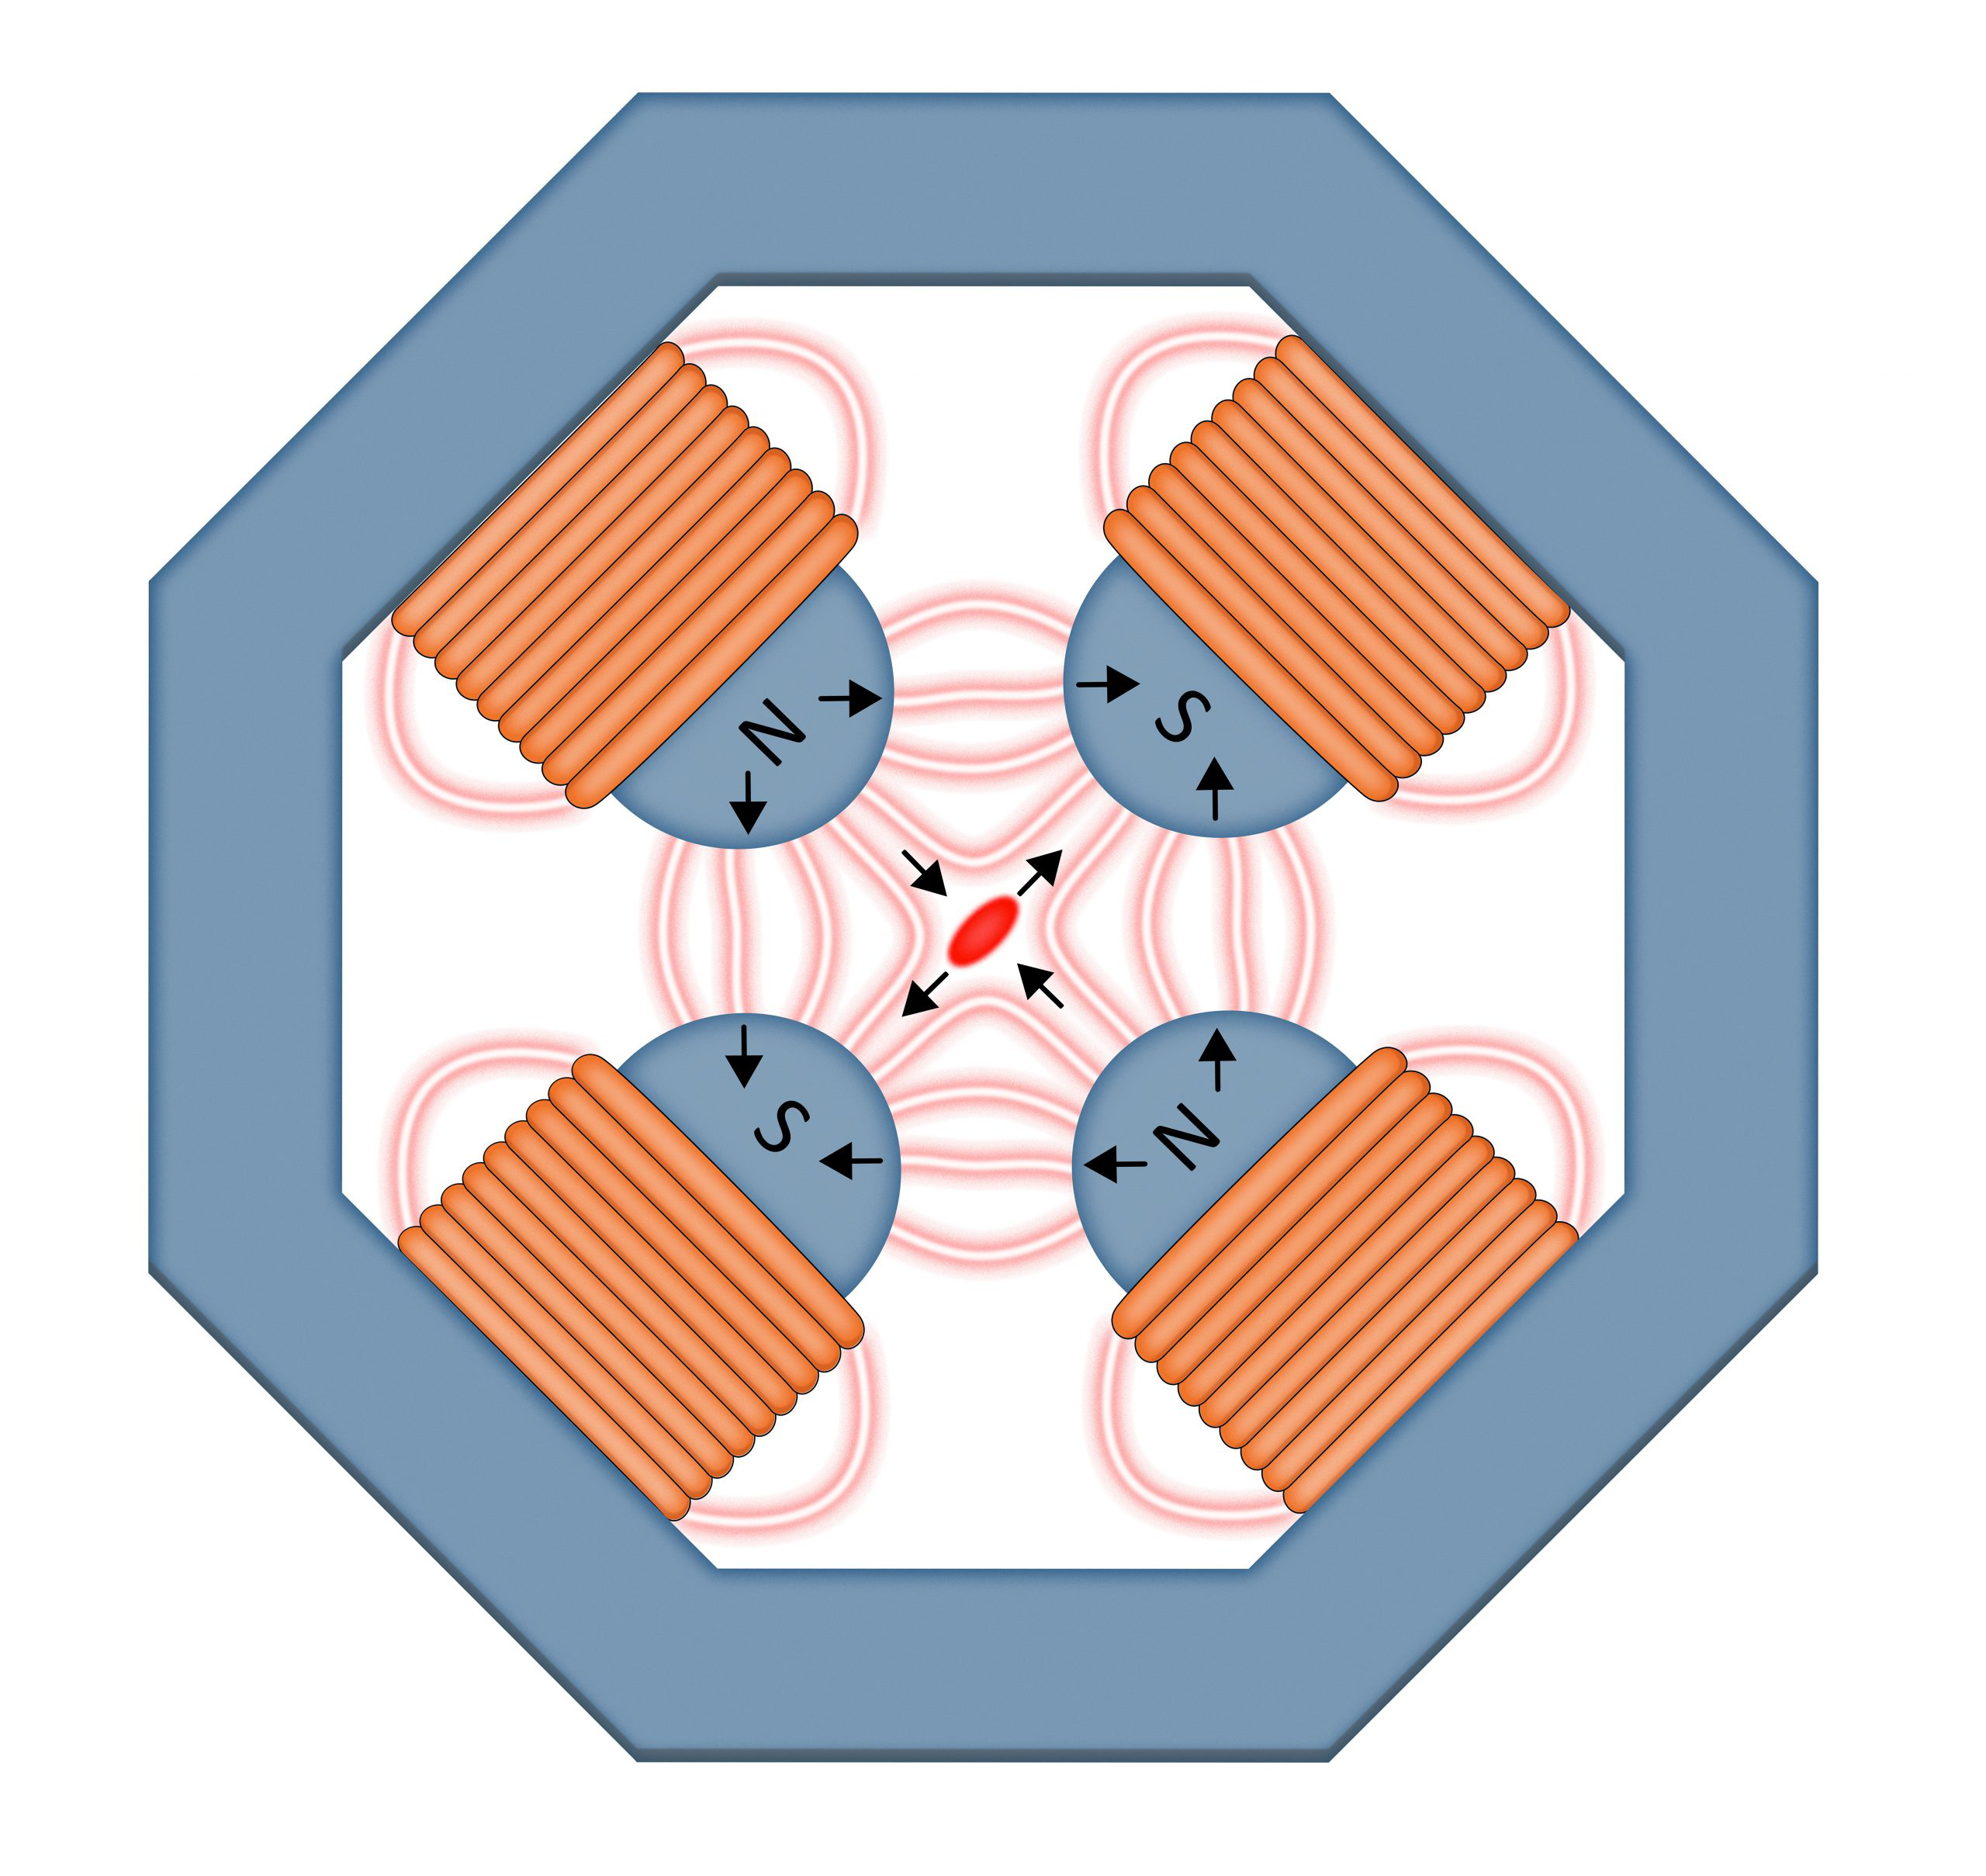
\includegraphics[width=0.9\textwidth]{Problem_18/quadrupoles.png}
\end{minipage}
\begin{minipage}{0.4\textwidth}
\centering
\begin{tikzpicture}[scale=0.7]
    \draw[-Stealth] (-4,0) to (4,0);
    \draw[-Stealth] (0,-4) to (0,4);
    \filldraw[color=black, fill=black, ultra thick] (0,0) circle (0.05);
    \draw (-0.3,0.3) node{$O$} (3.8,0) node[above]{$x$} (0,3.8) node[left]{$y$};
    \draw[dashed] (-3,-3) to (3,-3) to (3,3) to (-3,3) to (-3,-3);
    \draw[very thick, -Stealth] (-2.7,-2.7) to (-3.3,-3.3);
    \draw[very thick, -Stealth] (2.7,2.7) to (3.3,3.3);
    \draw[very thick, Stealth-] (2.7,-2.7) to (3.3,-3.3);
    \draw[very thick, Stealth-] (-2.7,2.7) to (-3.3,3.3);
\end{tikzpicture}
\end{minipage} \\
Hình 1: Mô hình tứ cực từ: (Bên trái) Trong thực tế; (Bên phải) Trong bài toán. 
\end{center}

    \item \textbf{Chuyển động của hạt qua một tứ cực từ} \\
    Một hạt điện tích q chuyển động với một động lượng $p$ lớn theo hướng gần như song song trục $Oz$ của một tứ cực từ. Để đơn giản, ta xem rằng hạt đi qua một tứ cực từ chỉ chịu ảnh hưởng của tứ cực từ trong một vùng dài $L$ [với $L \ll p/(qg)$] theo trục $Oz$ và từ trường trong vùng này có thể xem như không đổi theo tọa độ $z$. 
\begin{center}
\definecolor{9de0ad}{HTML}{9de0ad}
\definecolor{547980}{HTML}{547980}
\definecolor{594f4f}{HTML}{594f4f}
\begin{minipage}{0.4\textwidth}
\centering
\begin{tikzpicture}[scale=1]
    \draw[thick, fill=9de0ad] (-0.3,-2) rectangle (0.3,2);
    \draw[thick, 547980, -Stealth] (0.3,1) to (4,0);
    \draw[thick, 547980, -Stealth] (-2,1) to (0.3,1);
    \draw[thick, 547980, -Stealth] (0.3,-1) to (4,0);
    \draw[thick, 547980, -Stealth] (-2,-1) to (0.3,-1);
    \draw[thick, 594f4f, -Stealth] (-2.5,0) to (4.5,0);
    \draw (-0.3,0.5) node[left]{$x$} (2,0.05) node[below]{$f_x$} (4.3,0) node[above]{$z$} (0,1.5) node{$L$};
\end{tikzpicture}
\end{minipage}
\hspace{0.05\textwidth}
\begin{minipage}{0.4\textwidth}
\centering
\begin{tikzpicture}[scale=1]
    \draw[thick, fill=9de0ad] (-0.3,-2) rectangle (0.3,2);
    \draw[thick, 547980, dashed] (0.3,1) to (-4,0);
    \draw[thick, 547980, -Stealth] (0.3,1) to (1.16,1.2);
    \draw[thick, 547980, -Stealth] (-2,1) to (0.3,1);
    \draw[thick, 547980, dashed] (0.3,-1) to (-4,0);
    \draw[thick, 547980, -Stealth] (-2,-1) to (0.3,-1);
    \draw[thick, 547980, -Stealth] (0.3,-1) to (1.16,-1.2);
    \draw[thick, 594f4f, Stealth-] (2,0) to (-4.5,0);
    \draw (-0.3,0.5) node[left]{$y$} (-1.8,0.05) node[below]{$-f_y$} (1.8,0) node[above]{$z$} (0,1.5) node{$L$};
\end{tikzpicture}
\end{minipage} \vspace{3mm} \\
Hình 2: Quỹ đạo của hạt trong mặt phẳng $xOz$ (bên trái) và $yOz$ (bên phải).
\end{center}
    Theo định luật Earnshaw, trong trường tĩnh điện (và tương tự với từ trường) sẽ không tồn tại một vị trí cân bằng bền. Hiểu đơn giản trong trường hợp này, chúng ta có thể chỉ ra rằng nếu như chuyển động của hạt theo phương $x$ có một vị trí cân bằng bền để hạt dao động quanh thì vị trí cân bằng tương tự theo phương $y$ sẽ không phải vị trí cân bằng bền (và ngược lại). Như vậy, tứ cực từ giống như một thấu kính kỳ lạ, hội tụ đối với phương $x$ và phân kỳ đối với phương $y$ (như hình 2). Hãy tìm các tiêu cự $f_x$ và $f_y$ ứng với mỗi phương của thấu kính này theo $g$, $q$, $p$ và $L$.
    \item \textbf{Hội tụ chùm tia} \\
    Để chùm tia đi qua hệ hội tụ, người ta thường sử dụng các tứ cực từ thành từng cặp đặt lệch nhau $\SI{90}{^\circ}$ và cách nhau một khoảng $d$ (xem hình 3). Độ lớn các tiêu cự của các tứ cực từ là $f$. Hãy tìm tiêu cự tương đương qua toàn hệ $f'_x$ và $f'_y$ theo $f$ và $d$, chỉ ra điều kiện để chùm tia này hội tụ theo từng phương.
\end{enumerate}

\begin{center}
\hspace{0.05\textwidth}
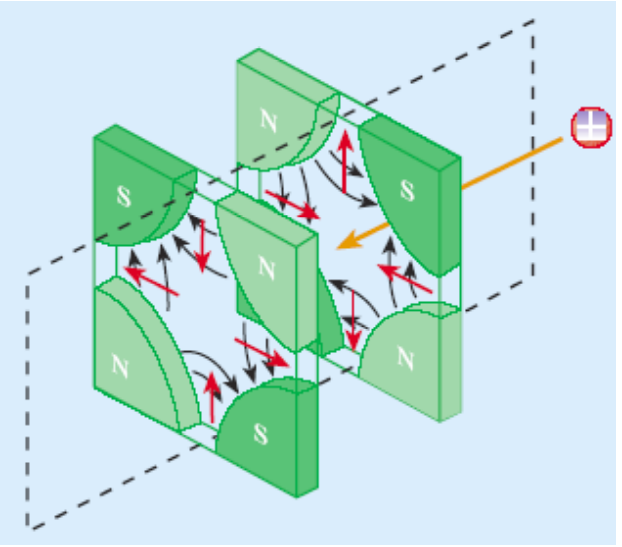
\includegraphics[width=0.38\textwidth]{Problem_18/two_quadrapole.png}
% \hspace{0.05\textwidth}
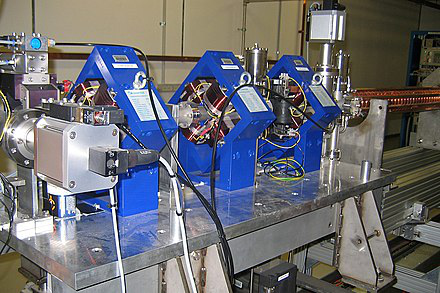
\includegraphics[width=0.5\textwidth]{Problem_18/Synchrotron_Quadrupole.png} \\
    Hình 3: Cặp tứ cực từ (bên trái) và máy gia tốc hạt hội tụ mạnh sử dụng các tứ cực từ (bên phải).
\end{center}

\begin{flushright}
    (Biên soạn bởi Bourbaki và Log)
\end{flushright}
\setcounter{equation}{0}
\begin{center}
    \normalcolor{\textbf{Bài giải}}
\end{center}
\begin{enumerate}
    \item Để tiện tính toán, ta đánh số các nam châm như hình dưới đây. \\
    \begin{figure}[!ht]
        \centering
        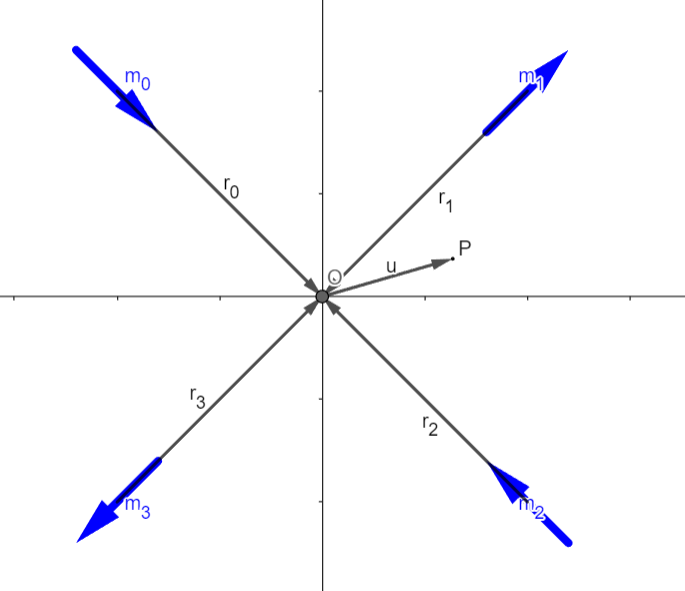
\includegraphics[scale = .5]{Problem_18/quadrupole.png}
      %  \caption{Caption}
    \end{figure}
    Từ trường tại điểm P có tọa độ $\Vec{r} = x\hat{x}+y\hat{y}$ là:
    \begin{equation} \label{eq1_Strong_Focusing}
        \Vec{B}= \sum_{i=0}^{3} \frac{\mu_0}{4\pi r_i'^5}\left[3(\Vec{m}_i\cdot \Vec{r'}_i)\Vec{r'}_i-\Vec{m}_i r_i'^2\right].
    \end{equation}
    Với $\Vec{r'}_i= \Vec{r}_i+\Vec{r}, \quad |\Vec{r}|/a \ll 1$, từ đây ta có
    \begin{equation} \label{eq2_Strong_Focusing}
        \frac{1}{r_i'^3}\approx\frac{1}{a^3}\left(1-\frac{3\Vec{r}_i \cdot \Vec{r}}{a^2}\right), \quad  \frac{1}{r_i'^5}\approx\frac{1}{a^5}\left(1-\frac{5\Vec{r}_i\cdot \Vec{r}}{a^2}\right).
    \end{equation}
        Thế (\ref{eq2_Strong_Focusing}) vào phương trình (\ref{eq1_Strong_Focusing}) ta thu được
    \begin{equation} \label{eq3_Strong_Focusing}
            \Vec{B} = \sum_{i=0}^{3} \frac{\mu_0}{4\pi}\left[\frac{3(\Vec{m}_i\cdot \Vec{r'}_i)\Vec{r'}_i}{a^5}\left(1-\frac{5\Vec{r}_i \cdot \Vec{r}}{a^2}\right)-\frac{\Vec{m}_i}{a^3}\left(1-\frac{3\Vec{r}_i \cdot \Vec{r}}{a^2}\right)\right].
    \end{equation}
    Ta lần lượt tính các số hạng thành phần của từ trường:
    \begin{equation} \label{eq4_Strong_Focusing}
        \Vec{m}_i\cdot \Vec{r}_i= (-1)^ip_m \cdot a\Longrightarrow \sum_{i=0}^{3}\Vec{m}_i \cdot \Vec{r'}_i= \sum_{i=0}^{3}\Vec{m}_i \cdot \Vec{r}+\sum_{i=0}^{3}(-1)^ip_m \cdot a=0,
    \end{equation}
    và
    \begin{equation} \label{eq5_Strong_Focusing}
    \begin{split}
        \sum_{i=0}^{3}(\Vec{m}_i \cdot \Vec{r'}_i)\Vec{r'}_i &=\sum_{i=0}^{3}(\Vec{m}_i \cdot \Vec{r}_i)\Vec{r}_i+\sum_{i=0}^{3}(\Vec{m}_i \cdot \Vec{r})\Vec{r}_i+\sum_{i=0}^{3}(\Vec{m}_i \cdot \Vec{r'}_i)\Vec{r}\\
        &=p_ma\sum_{i=0}^{3}(-1)^i\Vec{r}_i+\sum_{i=0}^{3}(\Vec{m}_i \cdot \Vec{r})\Vec{r}_i \\
        &=\sum_{i=0}^{3}(\Vec{m}_i\cdot \Vec{r})\Vec{r}_i= \sum_{i=0}^{3}\left[\Vec{r}\times (\Vec{r}_i \times\Vec{m}_i)+\Vec{m}_i(\Vec{r}_i \cdot\Vec{r})\right]\\
        &=\sum_{i=0}^{3}\Vec{m_i}(\Vec{r}_i \cdot\Vec{r}).
    \end{split}
    \end{equation}
    Thế (\ref{eq4_Strong_Focusing}) và (\ref{eq5_Strong_Focusing}) vào (\ref{eq3_Strong_Focusing}) và giữ lấy hệ thức bậc nhất theo $\Vec{r}$, ta thu được:
    \begin{equation} \label{eq6_Strong_Focusing}
        \begin{split}
            \Vec{B}&= \sum_{i=0}^{3} \frac{\mu_0}{4\pi}\left[\frac{6(\Vec{r}_i \cdot \Vec{r})\Vec{m}_i}{a^5}-\frac{15(\Vec{m}_i \cdot \Vec{r}_i )(\Vec{r}_i \cdot \Vec{r})\Vec{r}_i}{a^7}\right]\\
            &=\sum_{i=0}^{3} \frac{\mu_0}{4\pi}\left[\frac{6(\Vec{r}_i\cdot \Vec{r})\Vec{r}_i(-1)^ip_m}{a^6}-\frac{15(-1)^ip_m(\Vec{r}_i \cdot \Vec{r})\Vec{r}_i}{a^6}\right]\\
            &=-\sum_{i=0}^{3} \frac{\mu_0}{4\pi}\frac{9(\Vec{r}_i\cdot \Vec{r})\Vec{r}_i (-1)^ip_m}{a^6}\\
            &=- \frac{\mu_0}{4\pi}\frac{18p_m}{a^6}\left[(\Vec{r}_0 \cdot \Vec{r})\Vec{r}_0-(\Vec{r}_1\cdot \Vec{r})\Vec{r}_1 \right].
        \end{split}
    \end{equation} 
    Thay $\Vec{r}_0 = \frac{a}{\sqrt{2}}(\hat{x}-\hat{y})$ và $\Vec{r}_1= \frac{a}{\sqrt{2}}(\hat{x}+\hat{y})$, ta tìm được biểu thức từ trường
    \begin{equation} \label{eq7_Strong_Focusing}
        \Vec{B}=- \frac{\mu_0}{4\pi}\frac{9p_m}{a^4}\left[(x-y)(\Vec{x}-\Vec{y})-(x+y)(\Vec{x}+\Vec{y})\right]= \frac{9\mu_0}{2\pi}\frac{p_m}{a^4}(y\hat{x}+x\hat{y}).
    \end{equation}
    Hay
    \begin{equation} \label{eq8_Strong_Focusing}
        g = \dfrac{9 \mu_0}{2 \pi} \dfrac{9 p_m}{a^4}.
    \end{equation}
    Lực từ tác dụng lên một hạt điện tích có dạng $\Vec{F}\sim v\Vec{z}\times \Vec{B} \sim (\Vec{y}-\Vec{x})$. Do đó hạt có xu hướng dao động điều hòa theo phương $\hat{x}$ và chuyển động ra xa theo phương $\hat{y}$
    \item Vì lực từ không sinh công nên năng lượng của hạt $E= \text{const}$, vận tốc của hạt không đổi. Phương trình chuyển động của hạt sẽ được thu gọn thành
    \begin{equation} \label{eq9_Strong_Focusing}
        \frac{d \Vec{p}}{dt}= q \Vec{v} \times \Vec{B}.
    \end{equation}
    Chiếu phương trình trên theo 2 phương $x$ và $y$, đổi biến $t$ sang biến $z$ để triệt tiêu $v$, ta được
    \begin{align} \label{eq10_Strong_Focusing}
        \dfrac{d p_x}{dz} &= -qgx \Rightarrow \Delta p_x = -qgL x, \\
        \label{eq11_Strong_Focusing}
        \dfrac{d p_y}{dz} &= qgy \Rightarrow \Delta p_y = qgL y.
    \end{align}
    Khi hạt bay ra khỏi tứ cực từ, hạt gần như chuyển động thẳng đều, với góc chuyển động không đổi so với trục $z$, ta được
    \begin{align} \label{eq12_Strong_Focusing}
        &\dfrac{x}{f_x} = \dfrac{\Delta p_x}{p} \Rightarrow f_x = \dfrac{p}{qgL}. \\
        \label{eq13_Strong_Focusing}
        &\dfrac{y}{f_y} = -\dfrac{\Delta p_y}{p} \Rightarrow f_y = -\dfrac{p}{qgL}.
    \end{align}
    \item *Đối với phương $x$ của tứ cực từ thứ nhất: \\
    Sau khi đi qua tứ cực từ thứ nhất, chùm kia hội tụ tài đường thẳng cách tứ cực từ thứ hai một đoạn $g-f$. Đây là vật thật của thấu kính phân kỳ (ứng với  tứ cực từ thứ hai). Như vậy,
    \begin{equation} \label{eq14_Strong_Focusing}
        \dfrac{1}{d-f} + \dfrac{1}{f'_x} = -\dfrac{1}{f} \Rightarrow f'_x = \dfrac{f(f-d)}{d}.
    \end{equation}
    Như vậy, để chùm tia hội tụ theo phương $x$ sau khi qua hai tứ cực thì $d<f$.
    Tương tự đối với phương $y$, ta thu được kết quả:
    \begin{equation} \label{eq15_Strong_Focusing}
        \dfrac{1}{d+f} + \dfrac{1}{f'_y} = \dfrac{1}{f} \Rightarrow f'_y = \dfrac{f(f+d)}{d}.
    \end{equation}
    Theo phương $y$, chùm tia luôn hội tụ.
\end{enumerate}

\textbf{Biểu điểm}
\begin{center}
\begin{tabular}{|>{\centering\arraybackslash}m{1cm}|>{\raggedright\arraybackslash}m{14cm}| >{\centering\arraybackslash}m{1cm}|}
    \hline
    \textbf{Phần} & \textbf{Nội dung} & \textbf{Điểm} \\
    \hline
    \textbf{1} & Viết biểu thức tổng quát của từ trường gây ra bởi tứ cực (\ref{eq1_Strong_Focusing}) & $0.50$ \\
    \cline{2-3}
    & Khai triển nhỏ các số hạng (\ref{eq2_Strong_Focusing}) & $1.00$ \\
    \cline{2-3}
    & Tính các số hạng trong tổng (\ref{eq4_Strong_Focusing}) \& (\ref{eq5_Strong_Focusing}) & $1.00$ \\
    \cline{2-3}
    & Tìm biểu thức từ trường gần tâm của tứ cực từ và xác định $g$ (\ref{eq8_Strong_Focusing}) & $0.50$ \\
    \hline
    \textbf{2} & Lập luận về từ trường không sinh công và các hệ quả & $0.50$ \\
    \cline{2-3}
    & Viết phương trình biến thiên động lượng (\ref{eq9_Strong_Focusing}) & $0.50$ \\
    \cline{2-3}
    & Lấy tổng phương trình biến thiên động lượng theo hai phương (\ref{eq10_Strong_Focusing}) \& (\ref{eq11_Strong_Focusing}) & $1.00$ \\
    \cline{2-3}
    & Xác định tiêu cự của hai phương từ yếu tố hình học (\ref{eq12_Strong_Focusing}) \& (\ref{eq13_Strong_Focusing}) & $1.00$ \\
    \hline
    \textbf{3} & Khảo sát quỹ đạo của tia theo trục $Ox$ của tứ cực thứ nhất (\ref{eq14_Strong_Focusing}) & $1.00$ \\
    \cline{2-3}
    & Khảo sát quỹ đạo tia theo trục $Oy$ của tứ cực thứ nhất (\ref{eq15_Strong_Focusing}) & $1.00$ \\
    \hline
\end{tabular}
\end{center}


%% Reference %%
\bibliographystyle{plain}
\begin{thebibliography}{}
\bibitem{Hillert} Wolfgang Hillert. Transverse linear beam dynamics, 2021.
\bibitem{multipoles} \href{https://www.lhc-closer.es/taking_a_closer_look_at_lhc/0.magnetic_multipoles}{https://www.lhc-closer.es/taking\_a\_closer\_look\_at\_lhc/0.magnetic\_multipoles}
\end{thebibliography}

% \newpage
% {\normalcolor \textbf{CÂU 19}}\vspace{1.5mm}

% \setcounter{equation}{0}
% \input{Problem_19/P19}
% \setcounter{equation}{0}
% \begin{center}
%     \normalcolor{\textbf{Bài giải}}
% \end{center}
% \input{Problem_19/S19}

\newpage
{\normalcolor \textbf{CÂU 19+20 (16 điểm)}}\vspace{1.5mm}

\setcounter{equation}{0}
\textbf{Lý thuyết dây cho tương tác mạnh}

Theo Vật Lý hiện đại, thế giới tự nhiên được xây dựng dựa trên bốn lực tương tác cơ bản. Trong chương trình Vật Lý THPT, cũng như qua cuộc sống thường ngày, có lẽ các bạn đã không còn xa lạ với lực hấp dẫn và lực điện từ. Tuy nhiên, để giải thích các hiện tượng ở mức nguyên tử và nhỏ hơn, các nhà khoa học cần sử dụng thêm hai loại lực tương tác nữa: lực tương tác yếu và lực tương tác mạnh. Lý thuyết mô tả lực tương tác mạnh là {\it sắc động lực học lượng tử}, và theo lý thuyết này thì các hạt nhân nguyên tử -- hạt proton và hạt neutron -- có cấu tạo từ ba hạt quark, liên kết với nhau chủ yếu qua trường gluon. Các hạt được cấu tạo từ nhiều quark liên kết kiểu này có tên gọi chung là hadron. 

\begin{enumerate}
    \item \textbf{Quỹ đạo Regge của họ các hạt meson}\\
    Meson là các hạt hadron có cấu tạo từ hai quark. Xét một họ các hạt meson có liên hệ giữa khối lượng bình phương $M^2$ và spin $S$ (giá trị momen động lượng nội tại, tính theo đơn vị hằng số Planck rút gọn $\hbar$) như hình \ref{fig01}. Liên hệ này gần như tuyến tính $S = \alpha_0 + \alpha M^2$, là đặc trưng của tính chất quỹ đạo Regge, được quan sát trên rất nhiều họ các hạt meson khác nhau.

\begin{figure*}[!htbp]
\centering
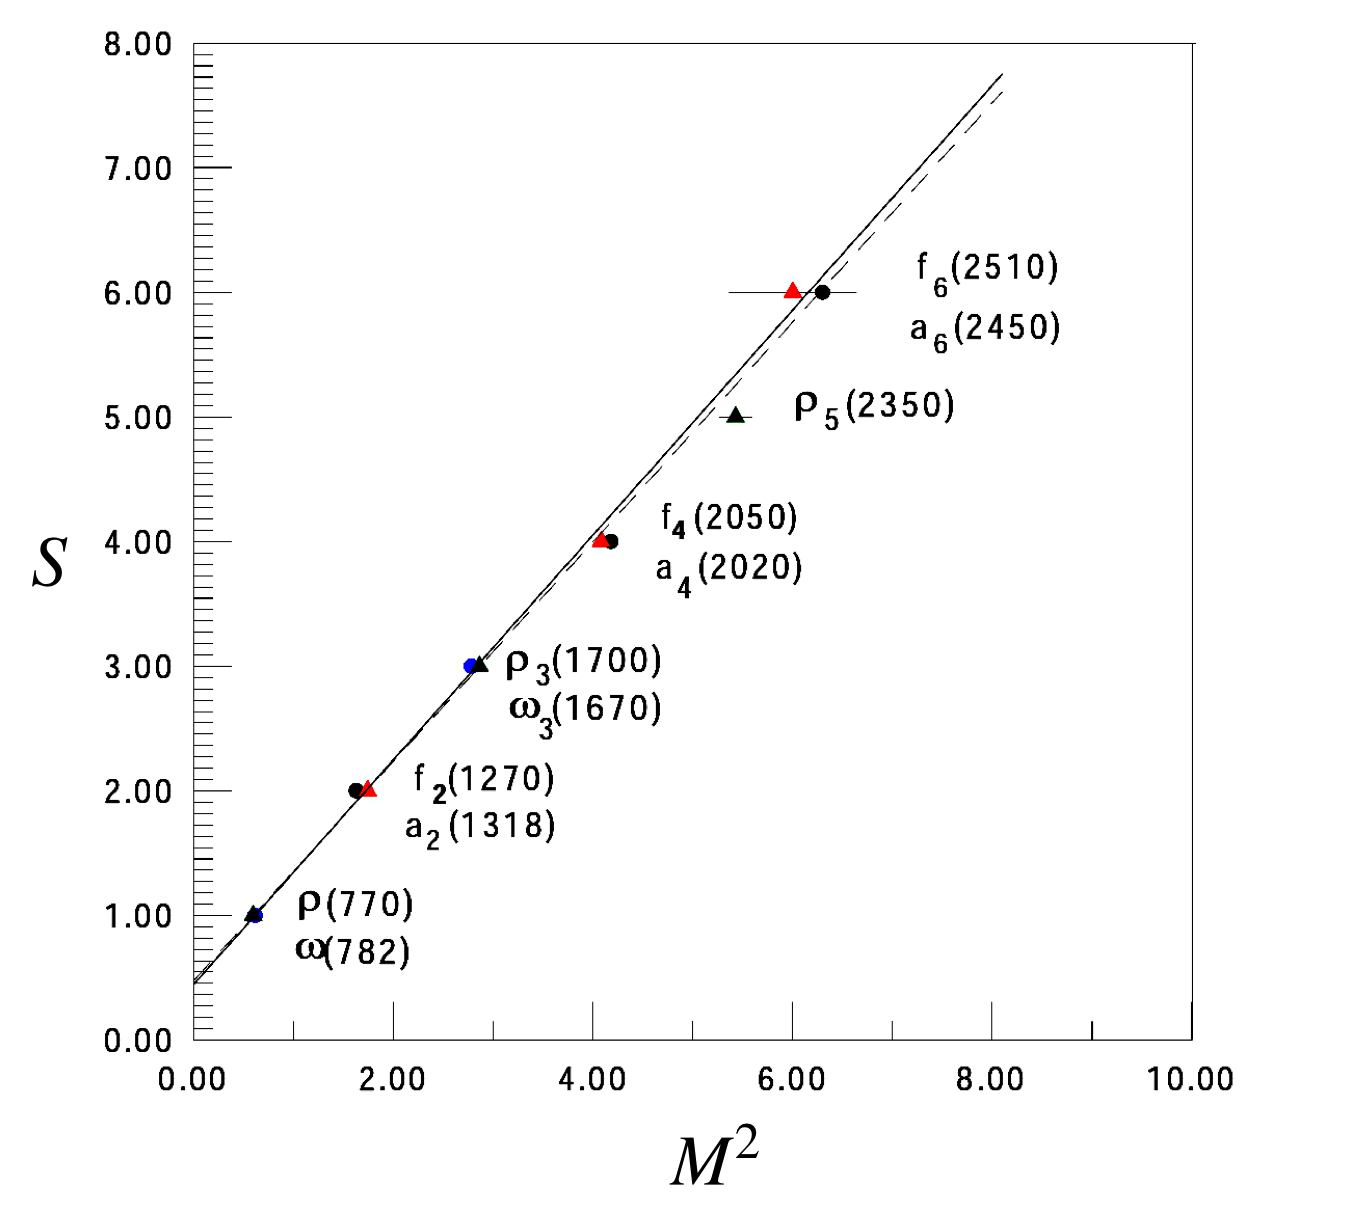
\includegraphics[width=0.6\textwidth]{Problem_20/fig01.png}%
\caption{Đồ thị Chew-Frautschi cho liên hệ gần như tuyến tính giữa khối lượng bình phương $M^2$ và spin (giá trị momen động lượng nội tại) $S$ của một họ các hạt meson.} %\cite{refId0}}
\label{fig01}
\end{figure*}
    
    Cho biết $M^2$ được tính theo đơn vị $($GeV$/c^2)^2$ với $c$ là giá trị vận tốc ánh sáng và $1$GeV $=1.60\times 10^{-10}$J. Hãy xác định hệ số tỉ lệ $\alpha$ của họ các meson trong hình \ref{fig01}. 
    
    \item \textbf{Mô hình dây tương đối tính của meson}\\
    Thành phần $\alpha M^2$ trong biểu thức của $S$ có thể được giải thích thông qua một mô hình dây quay tròn tương đối tính, như mô tả ở hình \ref{fig02}. Cụ thể, trong mô hình này, hai quark được nối với nhau bằng một ống dòng trường gluon tạo thành một dây có hai đầu nặng. Giả sử rằng các quark là những chất điểm có khối lượng nghỉ rất nhỏ $m \rightarrow 0$, và ống dòng trường gluon có mật độ năng lượng nghỉ $\lambda$ trên đơn vị chiều dài. Xét trạng thái chuyển động của hai quark là ở trên cùng một đường tròn, đứng yên trong hệ quy chiếu quan sát.

    \begin{figure*}[!htbp]
\centering
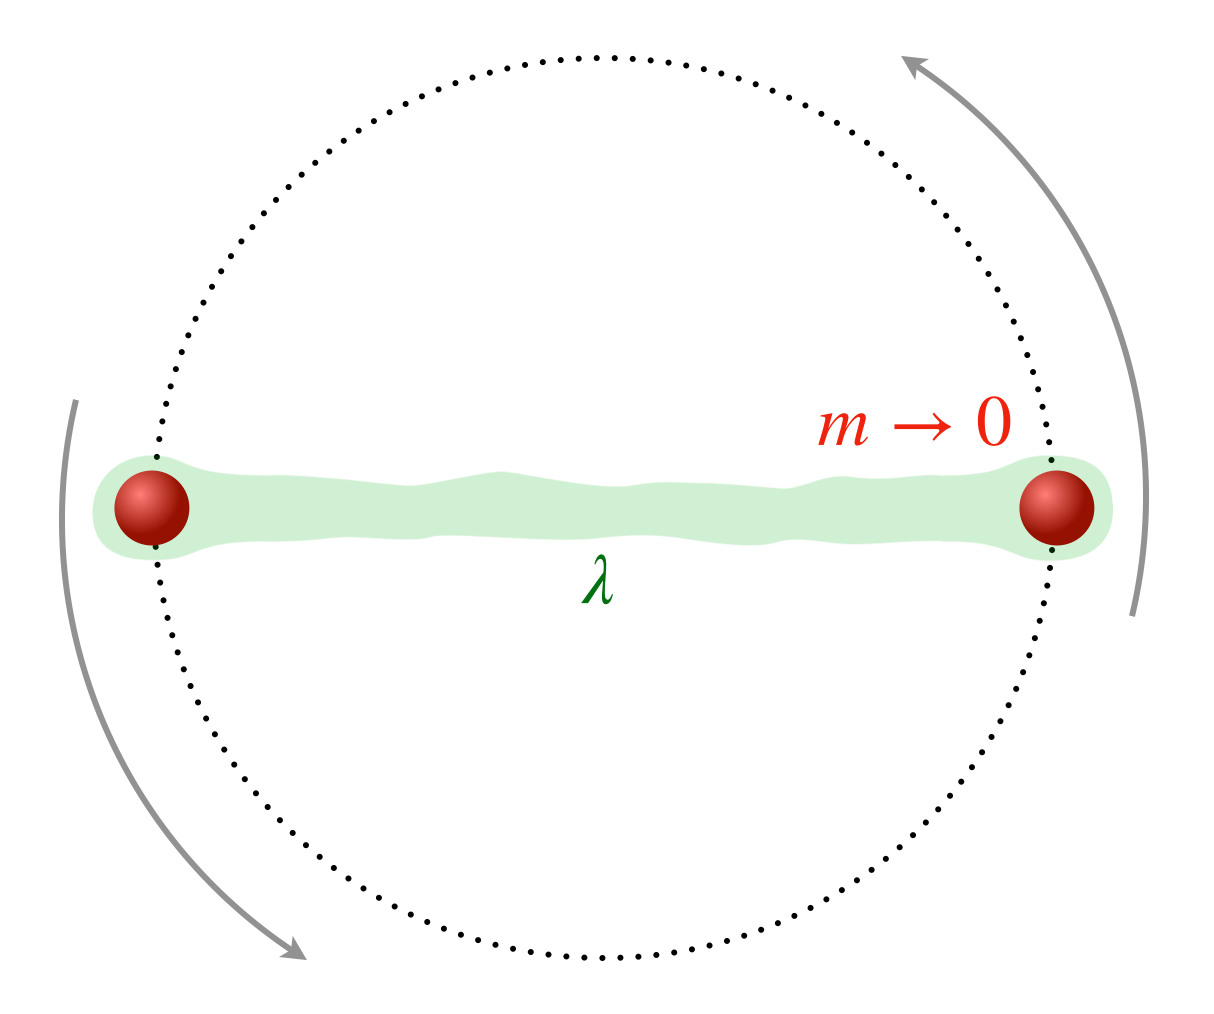
\includegraphics[width=0.6\textwidth]{Problem_20/fig02.png}%
\caption{Mô hình dây quay tròn tương đối tính của hạt meson, với giả sử rằng hai quark có khối lượng nghỉ $m\rightarrow 0$ và chuyển động trên cùng một đường tròn. Dây dự trữ mật độ năng lượng nghỉ $\lambda$ trên đơn vị chiều dài.}
\label{fig02}
\end{figure*}

    a/ Nếu momen động lượng của dây quay quanh tâm đường tròn là $J$, hãy xác định năng lượng $E$ của dây (cùng hai quark) trong hệ quy chiếu quan sát theo momen động lượng $J$ và mật độ năng lượng nghỉ $\lambda$. Bạn cần phải chứng minh rằng sự phụ thuộc của kết quả này vào khối lượng nghỉ $m$ các quark sẽ biến mất khi $m \rightarrow 0$.

    b/ Chúng ta liên hệ khối lượng $M$ của hạt meson với năng lượng $E$ của dây theo công thức tương đương năng - khối lượng Einstein $E=Mc^2$, và spin $S$ của meson với momen động lượng $J/\hbar$ của dây (tính theo đơn vị hằng số Planck rút gọn). Hãy xác định mật độ năng lượng nghỉ $\lambda$ theo giá trị $\alpha$ đã tìm được từ ý 1 của bài tập này.

    c/ Hãy xác định chiều dài $L$ của dây theo momen động lượng $J$ và hệ số $\alpha$. 
    
    \item \textbf{Nhiệt độ Hagedorn}\\
    Tương tác mạnh, như tên gọi của nó, là vô cùng mạnh -- ta gần như không thể quan sát được một hạt quark đơn lẻ ở trạng thái tự do, là đặc trưng cho tính chất giam cầm. Tuy nhiên, ở một giá trị nhiệt độ $T_{H}$ đủ lớn, được gọi là nhiệt độ Hagedorn, thì tương tác mạnh sẽ mất đi tính chất giam cầm và các quark sẽ được giải phóng, trở nên tự do -- hệ {\it sắc động lực học lượng tử} khi ấy sẽ ở trạng thái quark-gluon plasma.

    Ở các ý tiếp theo, chúng ta không những sẽ phải giải quyết một câu hỏi toán thống kê cụ thể, mà còn sẽ phải hiểu ý nghĩa Vật Lý của kết quả. Các bạn sẽ được cung cấp rất nhiều kiến thức mới, và yêu cầu phải sử dụng được chúng để giải quyết những câu hỏi.

    a/ Thay vì chỉ quay vòng quanh như mô hình tương đối tính trong hình \ref{fig02}, dây lượng tử có năng lượng và momen động lượng phụ thuộc vào trạng thái dao động của nó. Các giá trị momen động lượng khả dĩ của dây lượng tử (tính theo đơn vị hằng số Planck rút gọn) là tập hợp số nguyên không âm $J/\hbar =0,1,2,...$, và số lượng $\mathcal{N}[J/\hbar]$ các trạng thái dao động độc lập khác nhau cho mỗi giá trị momen động lượng $J/\hbar>0$ là bằng với số lượng các cách viết $J$ theo tổng của các số nguyên dương ($\mathcal{N}[0]=1$, tương ứng với trạng thái nền duy nhất). Các số hạng trong biẻu diễn tổng có thể lặp lại, nhưng các hoán đổi vị trí khác nhau chỉ được tính là một cách viết. Đây chỉ là một trong rất nhiều các liên hệ kỳ thú và sảng khoái giữa lý thuyết dây và lý thuyết số học.

    Chúng ta minh họa với $J/\hbar=4$. Có $5$ cách khác nhau để biểu diễn số $4$ theo tổng các số nguyên dương, là $1+1+1+1$, $1+1+2$, $1+3$, $2+2$, và $4$, cho nên $\mathcal{N}[4]=5$. Chú ý rằng, các trạng thái dao động khả dĩ của dây có thể xảy ra theo các phương khác nhau trong không gian, nhưng phép đếm $\mathcal{N}[J/\hbar]$ trên của chúng ta không hề đả động tới. Đây là một đơn giản hóa của bài tập. 

    Hãy xác định giá trị $\mathcal{N}[5]$, $\mathcal{N}[6]$, và $\mathcal{N}[7]$.

    b/ Hãy thành lập biểu thức ước tính chiều dài dây trung bình $\langle L \rangle$ ở nhiệt độ $T$, theo hàm $\mathcal{N}[J/\hbar]$, hệ số $\alpha$, hằng số Boltzmann $k_B$ và giá trị nhiệt độ $T$. Sử dụng kết quả đã tìm được ở ý 2a cho năng lượng $E$ dây quay tròn tương đối tính để ước tính năng lượng dây lượng tử, và 2c cho chiều dài $L$ dây quay tròn tương đối tính để ước tính chiều dài dây lượng tử, theo momen động lượng $J$ và hệ số $\alpha$. Giả sử rằng khi hệ {\it sắc động học lượng tử} ở nhiệt độ $T$ cân bằng thống kê thì xác suất dây sở hữu mỗi trạng thái mang năng lượng $E$ sẽ tuân theo phân bố Maxwell-Boltzmann -- tỉ lệ với $\exp(-E/k_B T)$.  

    c/ Chúng ta có thể xấp xỉ hàm $\mathcal{N}[J/\hbar]$ theo công thức Hardy-Ramanujan:
    \begin{equation}
        \mathcal{N}[J/\hbar] \approx \frac1{4\sqrt{3}(J/\hbar)} \exp \left[ \pi \sqrt{\frac{2(J/\hbar)}{3}} \right] \ ,
    \end{equation}
    áp dụng tốt nhất khi $J/\hbar \gg 1$. %\cite{LondonMathematical}
    
    Với kết quả tìm được ở ý 3b, vận dụng suy luận Vật Lý, hãy ước tính xem ở giá trị nhiệt độ bằng bao nhiêu thì các quark sẽ được giải phóng khỏi tính chất giam cầm. So sánh giá trị tìm được với nhiệt độ Hagedorn $T_H \sim 1.7 \times 10^{12}$K suy ra từ giả lập và thực nghiệm. %\cite{hadrons}
    
\end{enumerate}
    

\begin{flushright}
    (Biên soạn bởi XOONG)
\end{flushright}
\setcounter{equation}{0}
\begin{center}
    \normalcolor{\textbf{Bài giải}}
\end{center}
\textbf{Lý thuyết dây cho tương tác mạnh}

\begin{enumerate}
    \item \textbf{Quỹ đạo Regge của họ các hạt meson}\\
    Từ đồ thị trong hình \ref{fig01}, ta ước tính được $S/M^2 \approx 1$ theo đơn vị $($GeV$/c^2)^{-2}$, tức $\alpha \approx 3.15 \times 10^{53} \si{kg^{-2}}$. 
    
    \item \textbf{Mô hình dây tương đối tính của meson}\\
    Đây là một bài tập rất khó, yêu cầu bạn phải biết về liên hệ giữa lực và biến đổi chuyển động trong lý thuyết tương đối hẹp, cũng như áp dụng sự tương đương năng - khối lượng -- dây dự trữ mật độ năng lượng nghỉ $\lambda$ trên đơn vị chiều dài, tức nó cũng sở hữu khối lượng nghỉ $\lambda/c^2$ trên đơn vị chiều dài.
    
    a/ Gọi vận tốc của các quark là $\vec{v}$, đặt $\beta = v/c$ và $\gamma =  \left(1-\beta^2\right)^{-1/2}$. Dây dự trữ mật độ năng lượng nghỉ $\lambda$ trên đơn vị chiều dài, tức ý nghĩa Vật Lý của $\lambda$ chính là lực căng dây trong hệ quy chiếu nghỉ. Lực căng dây trong hệ quy chiếu quan sát tại vị trí đầu dây nối với các quark là $\lambda/\gamma$, gây nên biến thiên động lượng $\vec{p} =  \gamma m \vec{v}$ các quark:
    \begin{equation} \label{eq1_String_theory}
        \frac{\lambda}{\gamma} = \left| \ \frac{d}{dt} \vec{p} \ \right| = \frac{\gamma m v^2}{R} \ \ \Longrightarrow \  \ L  = \gamma^2 \beta^2 \frac{2mc^2}{\lambda} .
    \end{equation}
    Ở đây, $R$ là bán kính đường tròn, có độ dài bằng một nửa chiều dài dây $L$ (là đường kính đường tròn). Đóng góp năng lượng $E_{2q}$ và momen động lượng $J_{2q}$ của hai quark là:
    \begin{equation} \label{eq2_String_theory}
       E_{2q} = 2\gamma mc^2 \ , \ J_{2q} = 2 |\vec{p}| R = \gamma \beta m c L  \ .
    \end{equation}
    Đóng góp năng lượng $E_{d}$ và momen động lượng $J_{d}$ của ống dòng trường gluon là:
    \begin{equation} \label{eq3_String_theory}
    \begin{split}
       E_{g} & = 2 \int_0^R dr \left[ 1 - \left( \frac{r}{R}\beta \right)^2 \right]^{-1/2} \lambda = \left[ \frac{\arcsin(\beta)}{\beta} \right] \lambda L  \ ,
       \\
       J_{g} & = 2 \int_0^R dr \left\{ \left[ 1 - \left( \frac{r}{R}\beta \right)^2 \right]^{-1/2} \frac{\lambda}{c^2} \left( \frac{r}{R}\beta c \right) \right\} r = \left[ \frac{\arcsin(\beta) - \beta \left( 1-\beta^2 \right)^{1/2}}{4\beta^2} \right] \frac{\lambda L^2}{c} \ .
       \end{split}
    \end{equation}
    Tổng hợp lại, ta có năng lượng $E$ và momen động lượng $J$ của dây:
    \begin{equation} \label{eq4_String_theory}
    \begin{split}
    E &= E_{2q} + E_{g} =  \gamma \left[ 1 + \gamma \beta \arcsin(\beta) \right] 2 mc^2 \ ,
    \\
    J &= J_{2q} + J_{g} = \gamma \beta \left\{ 1 + 
 \frac12 \gamma^3 \beta \left[ \arcsin(\beta) - \beta \left( 1-\beta^2 \right)^{1/2} \right] \right\} \frac{2m^2c^3}{\lambda} \ ,
    \end{split}
    \end{equation}
    với giá trị của $L$ được thế bằng công thức tìm được ở \eqref{eq1_String_theory}. Khi $m \rightarrow 0$, vận tốc hai quark sẽ tiến gần tới giá trị vận tốc ánh sáng $\beta \rightarrow 1$ và $\gamma \rightarrow \infty$, nên vì vậy ta có xấp xỉ ở bậc cao nhất theo khai triển $\gamma$:
    \begin{equation} \label{eq5_String_theory}
       E \approx \pi \gamma^2 m c^2 + \mathcal{O}(\gamma) \ \ , \ \ J  \approx \frac{\pi}{2} \gamma^4 \frac{m^2 c^3}{\lambda} + \mathcal{O}(\gamma^3) \ .
    \end{equation}
    Từ đây ta thu được gần đúng liên hệ tỉ lệ tuyến tính giữa năng lượng bình phương $E^2$ và momen động lượng $J$:
    \begin{equation} \label{eq6_String_theory}
        \left(2\pi \lambda c\right)^{-1} E^2 \approx J \ \ \Longrightarrow \ \ E = \left[ \left(2\pi \lambda c\right) J \right]^{1/2} \ .
    \end{equation}

    b/ Với $E=Mc^2$ và $J=S \hbar$, công thức \eqref{eq6_String_theory} trở thành:
    \begin{equation} \label{eq7_String_theory}
        \frac{c^3}{2\pi \lambda} M^2 \approx S \hbar \ \ \Longrightarrow \ \ \lambda = \frac{c^3}{2\pi \hbar \alpha} \ .
    \end{equation}

    c/ Để liên hệ $L$ với $J$, chúng ta sử dụng công thức \eqref{eq1_String_theory} và công thức \eqref{eq4_String_theory}:
    \begin{equation} \label{eq8_String_theory}
    L \xrightarrow{\gamma \rightarrow \infty} \gamma^2 \frac{2mc^2}{\lambda} \approx \left( \frac{8}{\pi}\frac{c}{\lambda} J \right)^{1/2} = \left( \frac{16\hbar^2 \alpha}{c^2} J \right)^{1/2}
    \end{equation}
    
    \item \textbf{Nhiệt độ Hagedorn}\\
    a/ $\mathcal{N}[5]=7$, do $5$ có thể được biểu diễn theo tổng $1+1+1+1+1$, $1+1+1+2$, $1+1+3$, $1+2+2$,$1+4$, $2+3$, và $5$. 
    
    $\mathcal{N}[6]=11$, do $6$ có thể được biểu diễn theo tổng $1+1+1+1+1+1$, $1+1+1+1+2$, $1+1+1+3$, $1+1+2+2$,$1+1+4$, $1+2+3$, $1+5$, $2+2+2$, $2+4$, $3+3$, và $6$. 
    
    $\mathcal{N}[7]=15$, do $7$ có thể được biểu diễn theo tổng $1+1+1+1+1+1+1$, $1+1+1+1+1+2$, $1+1+1+1+3$, $1+1+1+2+2$,$1+1+1+4$, $1+1+2+3$, $1+1+5$, $1+2+2+2$, $1+2+4$, $1+3+3$, $1+6$, $2+2+3$, $2+5$, $3+4$, và $7$.

    b/ Với công thức ở ý 2a là $E(\alpha,J/\hbar)$ và ở ý 2c là $L(\alpha,J/\hbar)$, thế thì ta có thể tính chiều dài dây trung bình $\langle L \rangle$ ở nhiệt độ cân bằng thống kê $T$ như sau:
    \begin{equation} \label{eq9_String_theory}
        \langle L \rangle = \frac{\displaystyle \sum_{J/\hbar=0}^{\infty} \mathcal{N}[J/\hbar] \exp\left[ - \frac{E(\alpha,J/\hbar)}{k_B T} \right] L(\alpha,J/\hbar)}{\displaystyle \sum_{J/\hbar=0}^{\infty} \mathcal{N}[J/\hbar] \exp\left[ - \frac{E(\alpha,J/\hbar)
        }{k_B T} \right]} \ .
    \end{equation}
    Cụ thể hơn:
    \begin{equation} \label{eq10_String_theory}
        E(\alpha,J/\hbar) = \left[ \frac{c^4}{\alpha} (J/\hbar) \right]^{1/2} \ \ , \ \ L(\alpha,J/\hbar) = \left[ \frac{16 \hbar^2 \alpha}{c^2} (J/\hbar) \right]^{1/2}  \ .
    \end{equation}

    c/ Áp dụng công thức Hardy-Ramanujan, xác suất dây có chiều dài $L(\alpha,J/\hbar) \propto (J/\hbar)^{1/2}$ khi $J/\hbar \gg 1$ là tỉ lệ với:
    \begin{equation} \label{eq11_String_theory}
    \mathcal{N}[J/\hbar] \exp\left[ - \frac{E(\alpha,J/\hbar)}{k_B T} \right] \approx \exp \left\{ \left[ \left(\frac{2\pi^2}{3}\right)^{1/2} - \frac1{k_B T} \left( \frac{c^4}{\alpha} \right)^{1/2} \right] (J/\hbar)^{1/2}\right\} \ ,
    \end{equation}
    tăng theo hàm mũ theo chiều dài khi bên vế phải sở hữu $[...]>0$:
    \begin{equation} \label{eq12_String_theory}
        T > \frac1{k_B} \left( \frac{3}{2\pi^2} \frac{c^4}{\alpha} \right)^{1/2} \equiv T_* \ .
    \end{equation}
    Nói cách khác, chiều dài trung bình của dây tiến tới vô cùng khi $T>T_*$. Dây dài vô hạn tức hai quark có thể cách xa nhau tùy ý, không còn giam cầm bởi lực tương tác mạnh nữa! Ước tính này cho ta kết quả $T_* \approx 4.5 \times 10^{12} \si{K} $, cùng bậc độ lớn với nhiệt độ Hagedorn, nhiệt độ mà các hadron sẽ ``tan chảy''.
\end{enumerate}

\textbf{Biểu điểm}
\begin{center}
\begin{tabular}{|>{\centering\arraybackslash}m{1cm}|>{\raggedright\arraybackslash}m{14cm}| >{\centering\arraybackslash}m{1cm}|}
    \hline
    \textbf{Phần} & \textbf{Nội dung} & \textbf{Điểm} \\
    \hline
    \textbf{1} & Xác định hệ số $\alpha$ từ đồ thị & $4.00$ \\
    \hline
    \textbf{2a} & Tìm chiều dài dây theo vận tốc \eqref{eq1_String_theory} & $1.00$ \\
    \cline{2-3}
    & Xác định đóng góp năng lượng và momen động lượng của hai quark \eqref{eq2_String_theory} & $0.50$ \\
    \cline{2-3}
    & Xác định đóng góp năng lượng và momen động lượng của dây \eqref{eq3_String_theory} & $1.00$ \\
    \cline{2-3}
    & Khảo sát các đại lượng khi khối lượng quark rất bé \eqref{eq5_String_theory} & $1.00$ \\
    \cline{2-3}
    & Đưa ra mối liên hệ giữa năng lượng và moment động lượng \eqref{eq6_String_theory} & $0.50$ \\
    \hline
    \textbf{2b} & Xác định $\lambda$ theo $\alpha$ \eqref{eq7_String_theory} & $1.00$ \\
    \hline
    \textbf{2c} & Xác định chiều dài $L$ của dây theo $J$ và $\alpha$ \eqref{eq8_String_theory} & $1.00$ \\
    \hline
    \textbf{3a} & Xác định giá trị $\mathcal{N}[5]$, $\mathcal{N}[6]$, và $\mathcal{N}[7]$ & $2.00$ \\
    \hline
    \textbf{3b} & Tính chiều dài trung bình của dây \eqref{eq9_String_theory} & $2.00$ \\
    \hline
    \textbf{3c} & Áp dụng công thức Hardy-Ramnujan xác định xác suất độ dài dây \eqref{eq11_String_theory} & $1.00$ \\
    \cline{2-3}
    & Đánh giá về nhiệt độ và biện luận \eqref{eq12_String_theory} & $1.00$ \\
    \hline
\end{tabular}
\end{center}

%% Reference %%
\bibliographystyle{plain}
\begin{thebibliography}{}
\bibitem{refId0} P. Desgrolard, M. Giffon, E. Martynov, and E. Predazzi. Exchange-degenerate regge trajectories: A fresh look from resonance and forward scattering regions. \textit{Eur. Phys. J. C}, 18(3):555–561, 2001.
\bibitem{LondonMathematical} \textit{Proceedings of the London Mathematical Society 2.1 (1918): 75-115.}
\bibitem{hadrons} \textit{Melting hadrons, boiling quarks: from Hagedorn temperature to ultra-relativistic heavy-ion collisions at CERN: with a tribute to Rolf Hagedorn. Springer Nature; 2016.}
\end{thebibliography}


\begin{center}
    \normalcolor{------------------------------------------------ HẾT ------------------------------------------------}
\end{center}

\newpage
\input{Acknowledgement}

\end{document}